\documentclass[11pt]{article}
\usepackage{amsfonts,amsmath,amssymb,amsthm}
\usepackage{graphicx,psfrag,epsf}
\usepackage{enumerate}
\usepackage{url} % not crucial - just used below for the URL
\usepackage{algorithm}
\usepackage{algpseudocode}
\usepackage{subfig}
\usepackage{authblk}
\usepackage{verbatim} %used to comment out unnecessary contents
\usepackage{helvet}
\usepackage[colorlinks=true,pagebackref,linkcolor=magenta]{hyperref}
\usepackage[sort&compress,comma,square,numbers]{natbib}
\usepackage{fullpage,fancyhdr}
\renewcommand{\familydefault}{\sfdefault}
\usepackage{color} %used to highlight changes
\usepackage{paralist}
\usepackage{lineno}
% \usepackage{todonotes}
\usepackage[font=small,labelfont=bf]{caption}
\usepackage[final,authormarkup=none]{changes}
\newcommand{\note}[2][]{\added[#1,remark={#2}]{}}
% \usepackage[nottoc,numbib]{tocbibind}
% \usepackage{flushend}


%better toc
% \usepackage{tocloft}
% \setlength\cftparskip{-1pt}
% \setlength\cftbeforesecskip{2pt}
% \setlength\cftaftertoctitleskip{4pt}


\pagestyle{fancy}
% \oddsidemargin=-0.5in
% \evensidemargin=-0.5in
\textwidth=6.5in
\headwidth=6.5in
\textheight=9.0in
\headheight=0.0pt
\topmargin=0.0in
\headsep=0.0in
\renewcommand{\headrulewidth}{0pt}

\setlength{\parindent}{0em}
\setlength{\parskip}{0.7em}

% % DON'T change margins - should be 1 inch all around.
% \addtolength{\oddsidemargin}{-.5in}%
% \addtolength{\evensidemargin}{-.5in}%
% \addtolength{\textwidth}{1in}%
% \addtolength{\textheight}{-.3in}%
% \addtolength{\topmargin}{-.8in}%


\providecommand{\sct}[1]{{\sc \texttt{#1}}}
\providecommand{\mt}[1]{\widetilde{#1}}
\providecommand{\mb}[1]{\boldsymbol{#1}}
\providecommand{\mc}[1]{\mathcal{#1}}
\newcommand{\Real}{\mathbb{R}}
\newcommand{\G}{C}
\newcommand{\K}{\mathcal{K}}
\newcommand{\LL}{\mathcal{L}}
\newcommand{\Migraine}{\sct{Migraine}}
\newcommand{\mtg}{\sct{m2g}}
\newcommand{\T}{^{\ensuremath{\mathsf{T}}}}           % transpose
\newcommand{\Linefor}[2]{%
    \State \algorithmicfor\ {#1}\ \algorithmicdo\ {#2} \algorithmicend\ \algorithmicfor%
}
\newcommand{\subfigimg}[3][,]{%
  \setbox1=\hbox{\includegraphics[#1]{#3}}% Store image in box
  \leavevmode\rlap{\usebox1}% Print image
  \rlap{\hspace*{12pt}\raisebox{\dimexpr\ht1-0\baselineskip}{#2}}% Print label
  \phantom{\usebox1}% Insert appropriate spcing
}

\newcommand{\Mgc}{\sct{Mgc}}
\newcommand{\Mgcp}{\sct{Mgc$_P$}}
\newcommand{\Mgcd}{\sct{Mgc$_D$}}
\newcommand{\Mgcm}{\sct{Mgc$_M$}}
\newcommand{\Hhg}{\sct{Hhg}}
\newcommand{\Dcorr}{\sct{Dcorr}}
\newcommand{\Mcorr}{\sct{Mcorr}}
\newcommand{\Mantel}{\sct{Mantel}}

\newcommand{\website}{\url{https://github.com/jovo/RankdCorr/}}

\newcommand{\jv}[1]{{\note{jv: #1}}}
\newcommand{\jovo}[1]{{\note{jv: #1}}}
\newcommand{\cs}[1]{{\note{cs: #1}}}

\newcommand{\mbx}{\ensuremath{\mb{x}}}
\newcommand{\mby}{\ensuremath{\mb{y}}}


\linenumbers



%environment
\newtheorem{thm}{Theorem}
\newtheorem{appThm}{Theorem}
\setcounter{appThm}{0}
\newtheorem{lem}{Lemma}
\newtheorem{cor}{Corollary}
\newtheorem*{defi*}{Properties}
\newtheorem{asn}{Assumption}
\newcommand*\mean[1]{\bar{#1}}

\renewcommand{\algorithmicrequire}{\textbf{Input:}}
\renewcommand{\algorithmicensure}{\textbf{Output:}}

\begin{document}

\def\spacingset#1{\renewcommand{\baselinestretch}%
{#1}\small\normalsize} \spacingset{1}

\title{\bf Dependence Discovery from Multimodal Data via  Multiscale Graph Correlation}
\author[1]{Cencheng Shen} %\thanks{cshen@temple.edu}}
\author[2]{Carey E. Priebe}% \thanks{cep@jhu.edu}}
\author[3]{Mauro Maggioni}%\thanks{mauro.maggioni@duke.edu}}
\author[4]{Joshua T. Vogelstein\thanks{jovo@jhu.edu}}
\affil[1]{Department of Statistics, Temple University}
\affil[2]{Department of Applied Mathematics and Statistics, Johns Hopkins University}
\affil[2]{Department of Mathematics, Duke University}
\affil[4]{Department of Biomedical Engineering and Institute for Computational Medicine, Johns Hopkins University}
\maketitle
\pagestyle{empty}

% \bigskip
\begin{abstract}
Understanding and discovering dependence between multiple properties or measurements is a fundamental task not just in science, but also policy, commerce, and other domains.
An ideal test for dependence would have the following properties:
(1) Theoretical consistency such that the testing power converges to $1$ under any dependency structure and dimensionality.
(2) Strong empirical performance on a wide variety of low- and high-dimensional simulations.
(3) Provides insight into the nature of the dependence, rather than merely a valid p-value.
%(4) Is robust to outliers (that is, the presence of many independent samples mixed among a few dependent samples).
(4) On real data, detects dependence when it exists, and does not detect dependence when it does not exist.
No existing test satisfies all of these properties.
In this paper we propose a novel dependence test statistic called ``Multiscale Graph Correlation'' (\Mgc), by combining the ideas of distance correlation with nearest-neighbor testing.
More specifically, we only use the distance correlations amongst the nearest-neighbors of each data point, yielding a sparse, and therefore regularized, matrix from which we can compute the test statistic.
We demonstrate that \Mgc~has all of the above properties via a series of theoretical proofs, numerical simulations, and real data experiments.  Specifically, we applied \Mgc~in several real applications: (i) detect dependence between brain disorder and hippocampus shape, (ii) determine whether either of two pipelines can detect dependence between brain activity and personality, and (iii) do not inflate non-existent dependence between resting activity and a spurious stimulation.  \Mgc~performs as well or better than previously proposed methods in essentially all theory, low-dimensional and high-dimensional simulations, and real data experiments.  \Mgc~is therefore poised to be useful in a wide variety of applications, requiring only data and a dissimilarity function for both measurement types.  Both MATLAB and R code are provided here: \website.
\end{abstract}
\jv{in above abstract application (iii), you write "`failing to detect"', I reworded it, as "`failing"' sounds as a negative word to me. delete this comment if you are ok with it}


\noindent%
{\it Keywords: testing independence, distance correlation, k-nearest-neighbor, local correlation coefficient, permutation test}
% \vfill

% \clearpage
\setcounter{tocdepth}{2}% paragraphs and above
{\small\tableofcontents}
% \addtocontents{toc}{\vspace{-3\baselineskip}}
% \listofchanges[style=list]



% submitting to science, we get 320 for content
% total: 455, need to remove >100 lines, almost entirely from results.


\newpage
\spacingset{1.45}


% 73 lines; target = 64
% \section{Introduction}

Detecting dependency among multiple data sets is one of the most important and fundamental tasks in computational statistics and data science.
Indeed, prior to embarking on a predictive machine learning investigation, one might first check whether any dependence is detectable; if not, high-quality predictions will be unlikely.
The founders of statistics first highlighted the importance of this task, starting with Pearson, who developed Pearson's Product-Moment Correlation statistic  \cite{Pearson1895}.  Since then, researchers have consistently developed new and improved methods (see \cite{Reimherr2013} for a recent review and discussion).

In the era of big data, several challenges emerge as particularly prevalent and therefore, problematic.
%
First, the dependencies between different modalities of data can be highly \textbf{non-linear}.  While this has always been the case, the relative abundance of data has led to an increased demand in checking for dependence in many previously uninvestigated settings.
%
Second, the \textbf{dimensionality} of individual samples is growing at exponential rates, with genomics and connectomics data, for example, often accruing millions or billions of dimensions per data point. At the same time, the \textbf{sample sizes} are not increasing proportionally, meaning that we often have datasets with very high-dimensions and relatively low sample size.
%
Third, the data are often \textbf{complicated}: networks, shapes, questionnaires, semi-structured text are all typical examples.
% this could improve.  possibly elaborating upon what we mean, eg, non-euclidean.
For example, we may desire to understand whether brain shape and disease status are related, so that we can develop prognostic biomarkers to combat the deleterious efforts of degenerative neurological disorders \cite{ParkEtAl2008}.
%
%Fourth, because the acquisition of data has became so easy, and quality control still typically requires human supervision, the modern datasets often exhibit a large number of \textbf{outliers}, that is, samples with egregious errors.
%
Fourth, because we will often have a data deluge, with myriad different measurements, it is important to be able to compute the results reasonably \textbf{efficiently}.
%
Fifth, when working with big data, statistical procedures often have hyper-parameters that require tuning.  Many such procedures lack any guidance in choosing the value of those hyper-parameters, thereby requiring users of the procedures to concoct their own heuristics. It is desirable that a procedure is \textbf{adaptive}, in that it can automatically set its hyper-parameters in a valid way.
%
Finally, as alluded to above, checking for dependence is rarely the final step in the analysis.  Frequently, investigators and analysts desire more than a simple p-value, rather, they desire some insight into the nature of the \textbf{dependence structure}, which can then inform them in terms of how to proceed.
%
% Thus, dependence tests that work in non-linear, high-dimensional, low sample size, complex datasets, even in the presence of many outliers, reasonably quickly, and automatically adaptive to the data, and provide insight in addition to valid p-values, are highly desirable. Moreover, w
We desire tests that satisfy the above desiderata, both in theory as well as in extensive simulations and real data problems.

% We desire tests for which we can prove they have all these properties. More specifically, we desire a consistent test for as large a class of problems as possible, meaning, we want a test whose power converges to one as sample size increases to infinity whenever the two disparate views of the data are indeed dependent, and does not converge when they are not dependent.
% And we desire  consistent tests for as large a class of dependence structures as possible, much larger than merely linear and low-dimensionality dependence, and including all sorts of objects, including shapes and graphs and vectors.
% In addition to asymptotic guarantees of the above, we desire superior finite sample performance, which we can assess in extensive simulations.  Finally, we desire that these tests provide guidance into our real data data scientific inquiries.
% , both in terms of discovering novel dependencies, and providing insight into the nature of those dependencies.


% and we can also demonstrate them both in extensive simulations and real data.

There are two key insights from the literature that we combine to develop our methodology that satisfies the above desiderata.  First, a collection of pairwise comparisons suffices to characterize a joint distribution \cite{Maa1996}.  Second, nonlinear manifolds can be approximated by local linear spaces \cite{Allard2012}.  Our approach, Multiscale Graph Correlation (\Mgc), leverages and improves upon recent developments from both subdisciplines of data science.



\jv{I made some changes in the paragraph below for better accuracy.}
\cs{why did you remove ``doesn't adapt to data?'', and complicated domains?  }
\jv{complicated domain is still there for dcorr.
For data adaptation, I removed it for now, because I actually think having an additional hyperparameter is not necessarily an advantage, i.e., performance surely improves with more parameters, but it will require good estimation. So data adaptation is the property of our method and not theirs, but I don't think it is a disadvantage for them. What do you think?}
\cs{definitely a disadvantage.}
% Two related and very recent approaches stand out for their abilities in dealing with the above challenges.


Interpoint pairwise comparison matrices have been used for over 100 years for various statistical purposes \cite{Maa1996}. Perhaps one of the earliest examples of using them for dependence testing comes from  Karl Pearson \cite{Pearson1895}, who created  a special case of something subsequently called a ``generalized correlation coefficient'' \cite{KendallBook}.
Generalized correlation coefficients start with $n$ pairs of observations $(x_i,y_i)$, where $x$'s and $y$'s both might vectors, shapes, networks, etc.  And then, a comparison function is defined for each.  Specifically, let $a_{ij}=\delta_x(x_i,x_j)$, and let $b_{ij}=\delta_y(y_i,y_j)$.  
% Specifically, let $a_{ij}$ to be \emph{some} function of $\mbx_i$ and $\mbx_j$  (for example, their Euclidean distance), and define $b_{ij}$ similarly for pairs $\mby_i$ and $\mby_j$. 
Thus, $A=\{a_{ij}\}$ and $B=\{b_{ij}\}$ are the $n \times n$ interpoint comparison matrices for $\mbx$ and $\mby$, respectively.  
Without loss of generality, assuming $A$ and $B$ have zero mean, a generalized correlation coefficient can then be written:
\begin{equation}
\label{generalCoef}
\G= \tfrac{1}{z} {\textstyle \sum_{i,j=1}^n a_{ij} b_{ij}},
\end{equation}
where $z$ is proportional to standard deviations of $A$ and $B$, that is $z=n^2\sigma_a \sigma_b$.
In words, $\G$ is the correlation across \emph{pairwise comparisons}, rather than the individual data samples.  
% That is, if we define $A$ and $B$ as the interpoint comparison matrices for \mbx~and \mby~respectively, then $\G$ is simply the correlation between elements of $A$ and $B$.
$\G$ has many well known special cases historically, including Pearson's  \cite{Pearson1895}, Spearman's \cite{Spearman1904},  Kendall's \cite{KendallBook}, and Mantel's correlation \cite{Mantel1967}. % which is widely used in biology and ecology.
% Three special cases of $\G$ are particularly popular for independence testing.  First, the \Mantel~coefficient \cite{Mantel1967}, a widely-used method in biology and ecology, defines $a_{ij}=||\mbx_i-\mbx_j||_{2}$.
% \Mantel, however, does not have any theoretical support for being a generally consistent test.
Recently, Szekely et al. \cite{SzekelyRizzoBakirov2007} extended these approaches, letting $\delta_x$ and $\delta_y$ to be the Euclidean distance, followed by subtracting the row means and column means, resulting in ``doubly centered'' distances.  Impressively, they proved that this ``distance correlation'' (\Dcorr) statistic is a consistent test for independence for any joint distribution (under suitable regularity conditions), that is, the \Dcorr's power approaches $1$ as sample size approaches infinity, for any joint distribution of finite dimension and finite second moments.
% \Dcorr, however, breaks down as the dimensionality of the data increases.  
% By adjusting the high-dimensional bias of \Dcorr, 
Szekely et al. \cite{SzekelyRizzo2013a} further proposed a modified version called \Mcorr, which they prove to be consistent even as the dimensions of $x$ and $y$ increase to infinity as well.
Moreover, because these distance based tests merely require a comparison function for both $x$ and $y$, Lyons was able to prove that they are consistent even in other metric spaces, including certain networks, shapes, and other complicated spaces \cite{Lyons2013}.
% work better in high-dimensions.
% The first, called ``distance correlation'' (\Dcorr), is a distance-based generalization of Pearson's product-moment correlation statistic \cite{RizzoSzekely2016}.
% \Dcorr~and its generalizations
Thus, existing generalized correlation coefficient based tests therefore
work well in high dimensions and low sample sizes, including in complicated domains, and are reasonably computationally efficient. But, empirically, they struggle in various non-linear settings, perhaps because they do not automatically adapt to the data.  Therefore, they also do provide insight into the nature of the dependence.


% In a separate academic lineage, manifolds have taken center stage.  A manifold is a topological space that can be approximated by a collection of local flat Euclidean spaces.  Although nonlinear manifold learning has been around since at least the 1950s \cite{TorgersonBook}, it rose to prominence in the early 2000s when Local Linear Embedding \cite{SaulRoweis2000} and Isomap \cite{TenenbaumSilvaLangford2000} popularized the notion that computing distances between neighboring points could enable ``unfolding'' the manifold to discover its structure.  Since then, a multitude of theoretical and empirical studies have devised different nonlinear dimensionality reduction techniques \cite{LeeVerleysen2007}, most of which are essentially generalized principal components analysis \cite{ScholkopfSmolaMuller1999}.  These approaches all require choosing the neighborhood size, a parameter of paramount importance for subsequent inference. Despite of many efforts to numerically determine the parameter, to our knowledge, no approach provides a principally justified method for choosing the neighborhood.



A deep insight that the generalized correlation coefficient tests  have yet to capitalized on, %although it has reaped benefits in myriad data science problems,
that could help address the above described limitations, 
is that nonlinear shapes can be approximated by \textbf{locally} linear ones \cite{Allard2012}.  Locality has been utilized for classification and regression  \cite{Stone1977}, data compression \cite{DaubechiesWaveletBook}, and recommender systems \cite{Sarwar2000}, to name a few of the myriad data science problems for which locality has already reaped benefits.
Moreover, it has become an invaluable tool in unfolding nonlinear geometry in many recent development of nonlinear embedding algorithms, dating back to the 1950s \cite{TorgersonBook}, and more recently making a resurgence with the advent of  Isomap \cite{TenenbaumSilvaLangford2000, SilvaTenenbaum2003}, Local Linear Embedding \cite{SaulRoweis2000, RoweisSaul2003}, and Laplacien eigenmaps \cite{BelkinNiyogi2003}, among many others. The concept of locality, while popular within certain fields has only entered into  testing very infrequently
% Most relevant to our work, a number of approaches to two-sample and dependence testing have utilized nearest-neighbor graphs
\cite{David1966,Friedman1983,Schilling1986}.  These approaches, like the distance correlation based ones, have the advantage of naturally operating on complicated data, because they only require a comparison function between observations.  They can also have strong theoretical guarantees. 
% \cite{deSilva2003,Allard2012}. 
However, these local testing approaches focus on two-sample testing, rather than dependence testing. 

The challenge associated with all of methods that employ locality is in choosing the appropriate scale (or neighborhood size) \cite{ShenVogelsteinPriebe2016}.  Even those approaches that do provide a mechanism for optimizing  neighborhood size often do so without any theoretical guarantees, and choose based on some surrogate function, rather than the exploitation task at hand. In either case, changing the neighborhood size for many of these algorithms typically requires running the entire algorithm again, rendering it computationally intractable. 
Thus, a gap remains in the literature: a dependence test that has all of the desirable properties of the distance based tests, but also performs well in highly nonlinear settings via adapting scale appropriately, thereby providing insight into the most informative neighborhood sizes for both understanding and subsequent inference purposes.  



% Moreover, these tests all fail to provide a convenient or automatic way to choose the appropriate neighborhood size.  This omission burdens the user of the test to come up with a heuristic, thereby greatly impairs their practical usages and finite sample performances. In fact, adaptively choosing the scale to regularize the data is a pernicious problem in essentially all existing local procedures,
% and a good choice of joint neighborhood can better unfold the nonlinearity and match data sets of multiple modality \cite{ShenVogelsteinPriebe2016}. A primary contribution of our work is an efficient mechanism both for looking across scales, and for choosing the optimal scale.


% In a separate academic linear, another dependence test named \Hhg~\cite{HellerGorfine2013} after its authors, performs very well on non-linear relationships, but falls short on some high-dimensional problems, may or may not work in complicated domains,
% is more time consuming to compute, and does not adapt
% % (again, does not have any explicit hyper-parameters),
% and also does not provide insight into the nature of the dependence structure.  Although these two approaches are currently considered the best tests for dependence, it is hopefully clear that a gap exists in the literature for an approach that satisfies all of the above desiderata.



% \jv{there are a few details in next paragraph we should discuss for better accuracy}
% \cs{ok}
% % XXX be super succint. this is like the first paragraph of the discussion. reduce by 2.5x or 3x
% More specifically,  we propose Multiscale Graph Correlation (\Mgc),
% which combines distance correlations with graph based tests, considers all locality scales, and chooses the best one.
% % \Mgc~therefore  naturally inherits the advantages of the global distance correlation tests---such as the consistency---while also enjoying the properties of graph-based tests to exclude non-local comparisons, efficiently for all definitions of local, and choosing the optimal neighborhood sizes.
% \Mgc~performs as well or better than the existing literature on each mentioned design goal, in theory, and extensive simulations.
% % More specifically, in a comprehensive simulation setting, \Mgc~is able to achieve superior finite-sample testing powers for data sets of nonlinearity, high-dimensionality with and small sample size, including outliers, quickly and adaptively.
% In real data experiments, we show that \Mgc~is able to uncover the underlying dependency between brain shape and disease that global tests were unable to detect, revealed the structure of dependence between brain networks and personality, and did not inflate the false positive rate when the dependencies are not there, unlike some other methods for fMRI analysis in \cite{EklundKnutsson2012}.
% % In this age of data, procedures that merely provide valid inferences are no longer sufficient; rather, the goal of running an analysis ought be provide additional insight to guide the practitioner to the next experiment or decision.  Crucially, \Mgc~does not merely provide valid p-values in myriad settings, rather, it also provides some insight into the nature of the dependence structure. To our knowledge, \Mgc~is the only dependence test that incorporates this important property, which we expect to be increasingly desirable as data becomes even more prevalent.
% We  expect \Mgc~to find values in a wide range of applications; to facilitate this, we provide open source MATLAB and R implementations of \Mgc~at~\website.

% 193 lines; target = 192
% \section{Results}
% \label{s:results}


\subsection*{Multiscale Graph Correlation}
\label{s:mgc}

All dependence tests start from the same setting: we observe $n$ pairs of observations $(\mbx_i,\mby_i)$, and we first desire to know whether the \mbx's and \mby's are independent of one another, and if so, we then desire to understand the nature of that dependence structure.


Multiscale Graph Correlation (\Mgc) combines generalized correlation coefficients with localilty.
% , in an effort to efficiently uncover local relationships and optimize the independence test.  
Specifically, let $R(a_{ij})$  be the ``rank'' of $\mbx_i$ relative to $\mbx_j$, that is, $R(a_{ij})=k$ if $\mbx_i$ is the $k^{th}$ closest point (or ``neighbor'') to $\mbx_j$, starting from $1$ to $n$, and  define $R(b_{ij})$ equivalently for the \mby's. For any neighborhood size $k$ around each \mbx~and any neighborhood size $l$ around each \mby, we define the rank-truncated pairwise comparisons:
\begin{equation}
\label{localCoef2}
    a_{ij}^k=
    \begin{cases}
      a_{ij}-\bar{a}^{k}, & \text{if } R(a_{ij}) \leq k, \\
      % -\bar{a}^{k}, & \text{otherwise};      
      0, & \text{otherwise};
    \end{cases} \qquad \qquad
    b_{ij}^l=
    \begin{cases}
      b_{ij}-\bar{b}^{l}, & \text{if } R(b_{ij}) \leq l, \\
      % -\bar{b}^{l}, & \text{otherwise};
      0, & \text{otherwise};
    \end{cases}
\end{equation}
where $\bar{a}^{k}$ and $\bar{b}^{l}$ are the local means such that  $\sum_{i,j=1}^{n} a_{ij}^k = \sum_{i,j=1}^{n} b_{ij}^l=0$.  We define a \emph{local} variant of any global generalized correlation coefficient by  excluding large distances: % up-to the centering scalars:
\begin{equation}
\label{localCoef}
\G^{kl}=\dfrac{1}{z_{kl}} {\textstyle \sum_{i,j=1}^n a_{ij}^k b_{ij}^l},
\end{equation}
where $z_{kl}=n^2 \sigma_a^k \sigma_b^l$,  with $\sigma_a^k$ and $\sigma_b^{l}$ being the standard deviations for the truncated pairwise comparisons. There are a maximum of $n^2$ different local correlations, one for each possible combination of $k$ and $l$ (more technical details of \Mgc~are in Appendix \ref{appen:mgc}).
% As an example, $\G^{kl}$ could be a local distance correlation by plugging in the respective $a_{ij}$ and $b_{ij}$ from the global distance correlation coefficient $\G$.
Among all $n^2$ local statistics, $\{\G^{kl}\}$, \Mgc~selects the best local statistic for testing. %(see Appendix \ref{appen:algorithms} for details on how to compute local correlations and estimate \Mgc).
Figure \ref{f:schematic} schematically illustrates \Mgc~on a particular nonlinear dependence structure.


\begin{figure}[htbp]
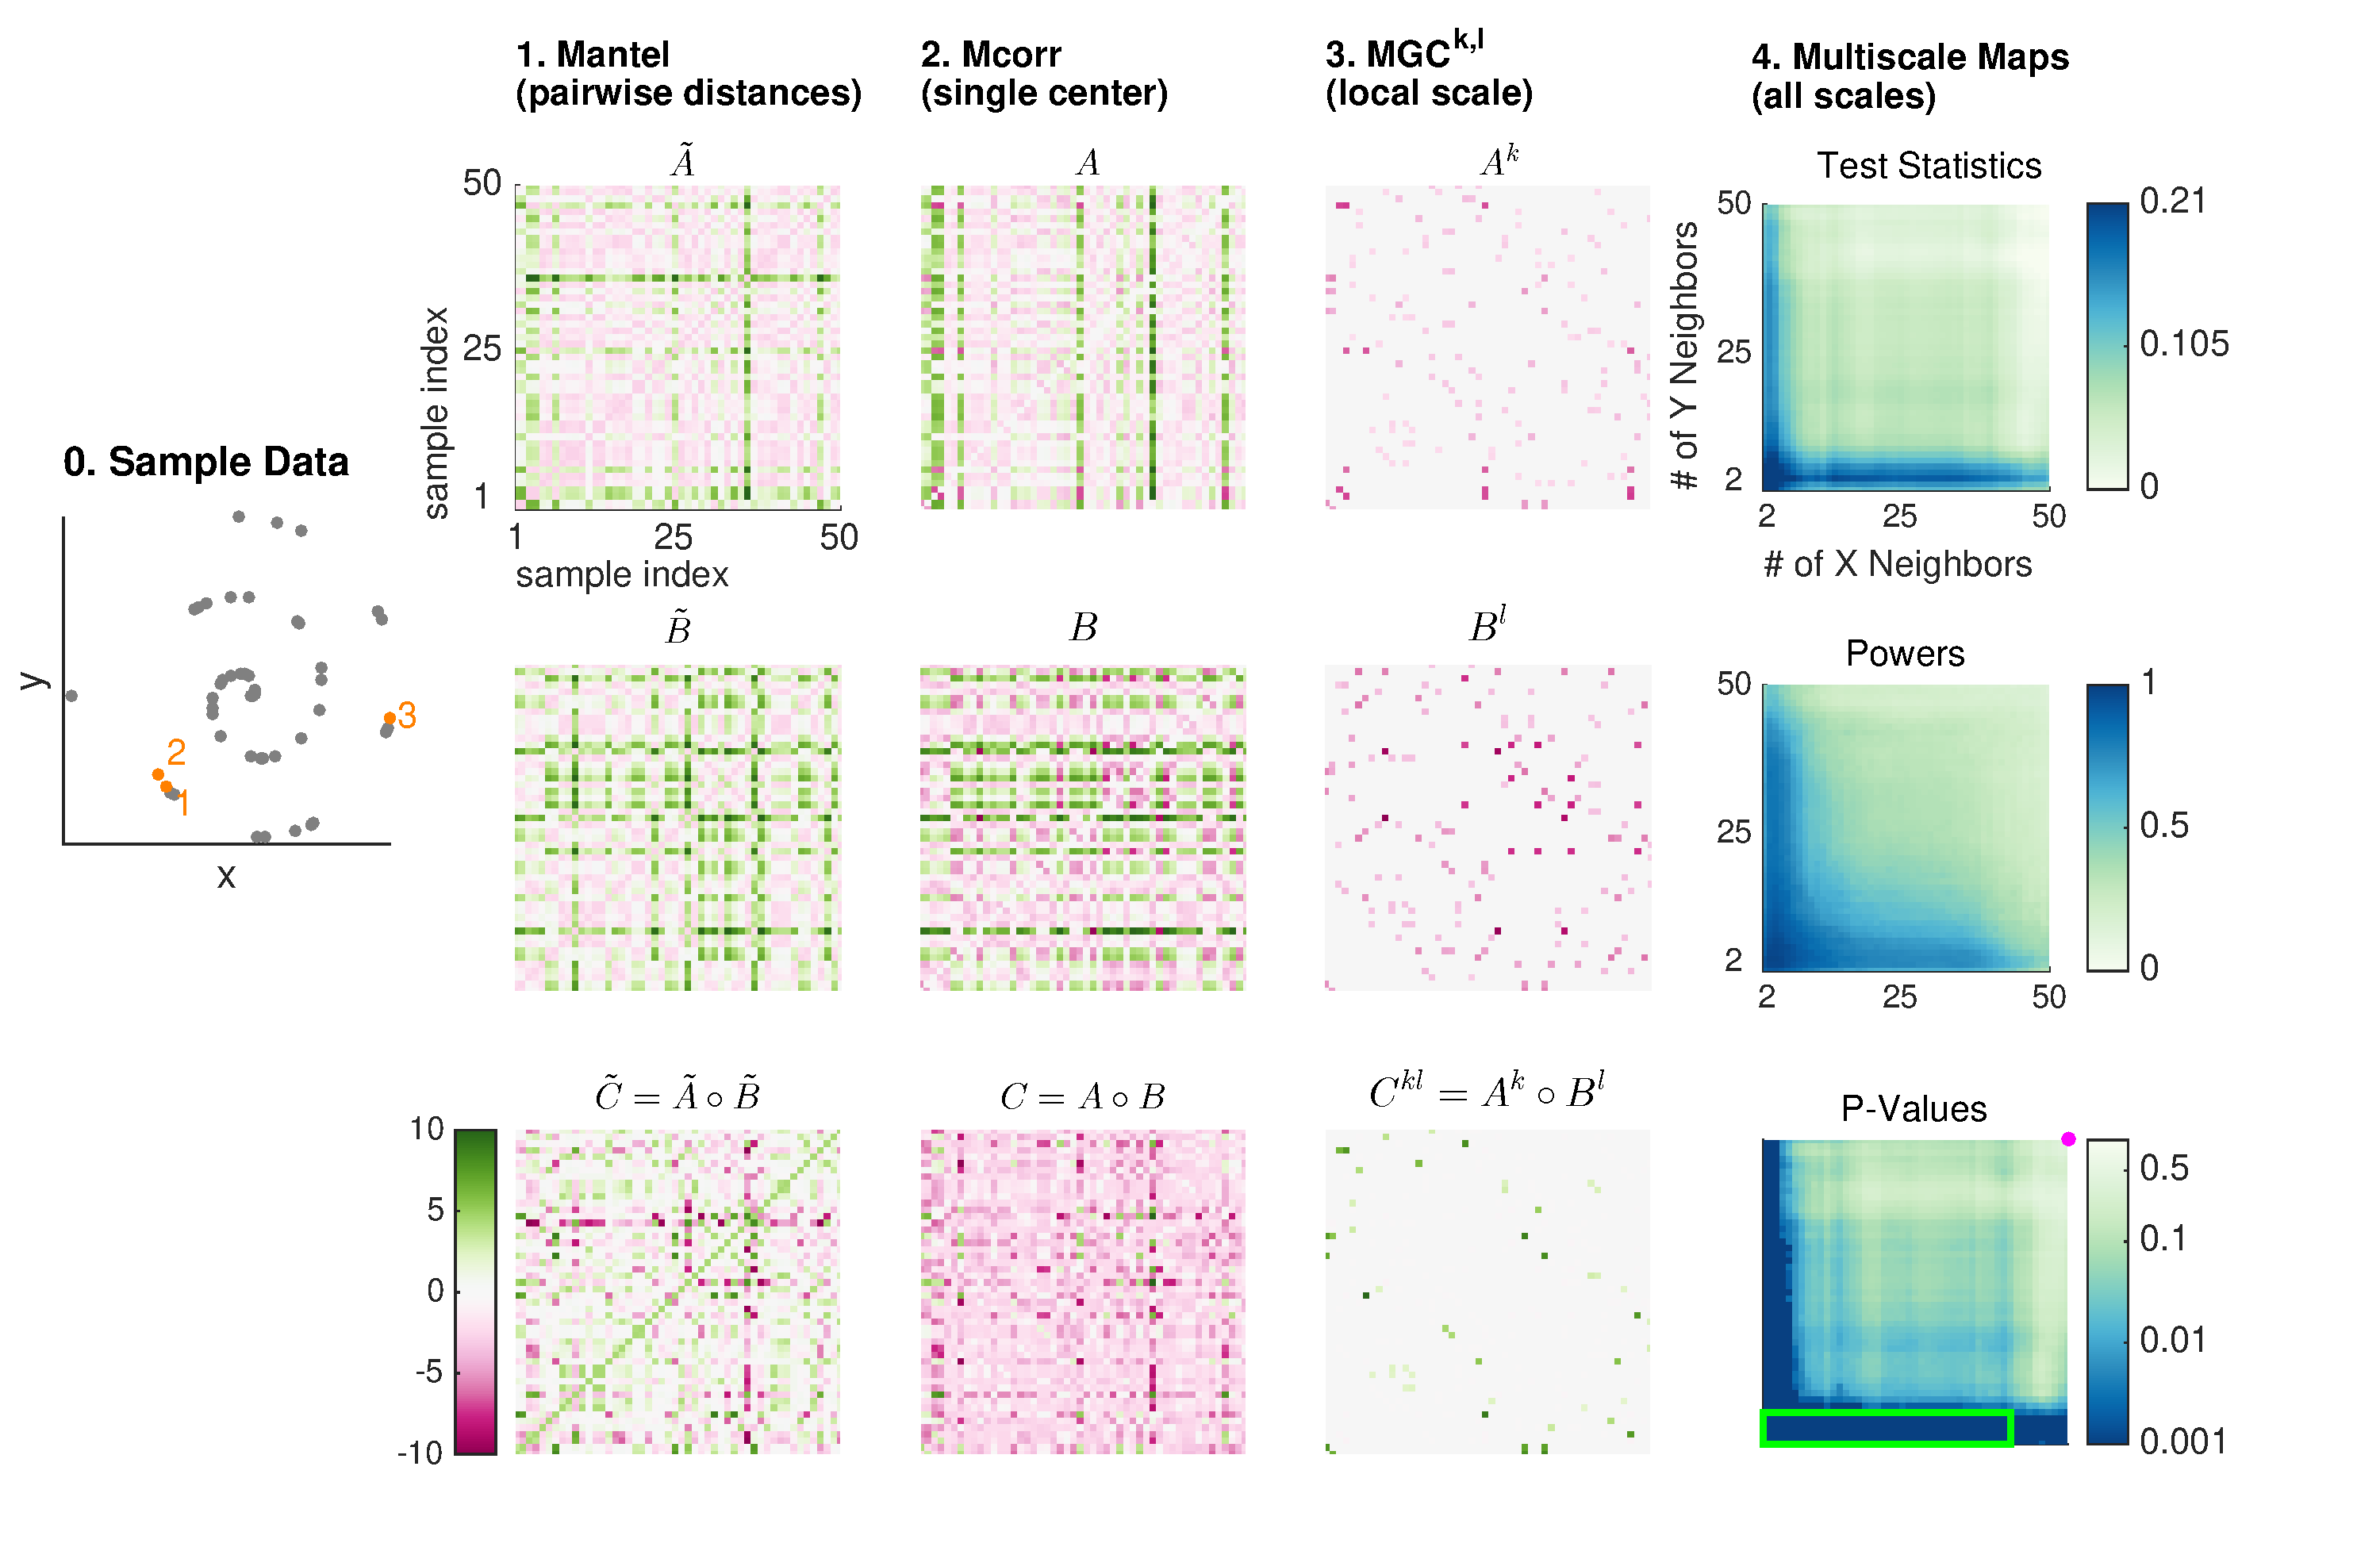
\includegraphics[width=1.0\textwidth]{../Figures/FigA}
% 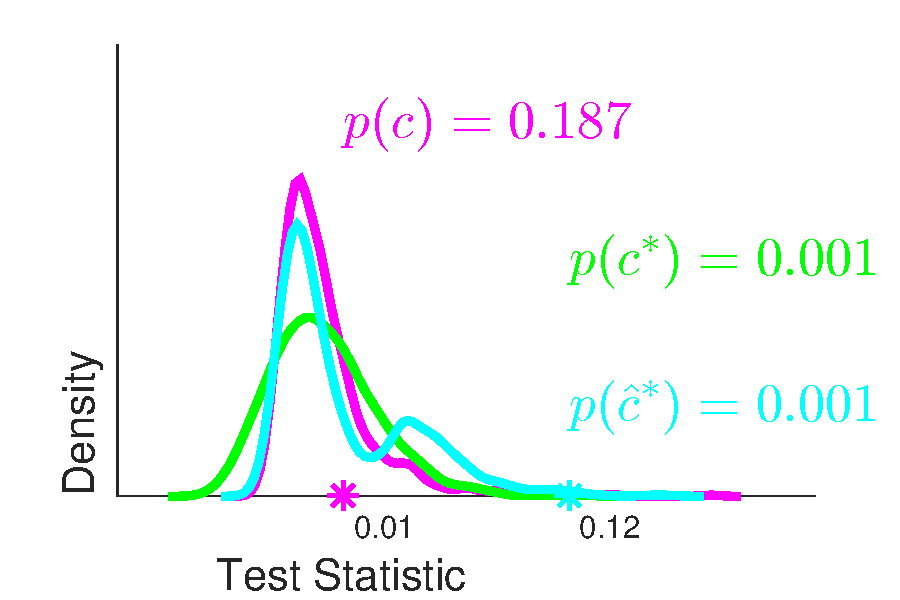
\includegraphics[width=1.0\textwidth]{../Figures/FigB}
% 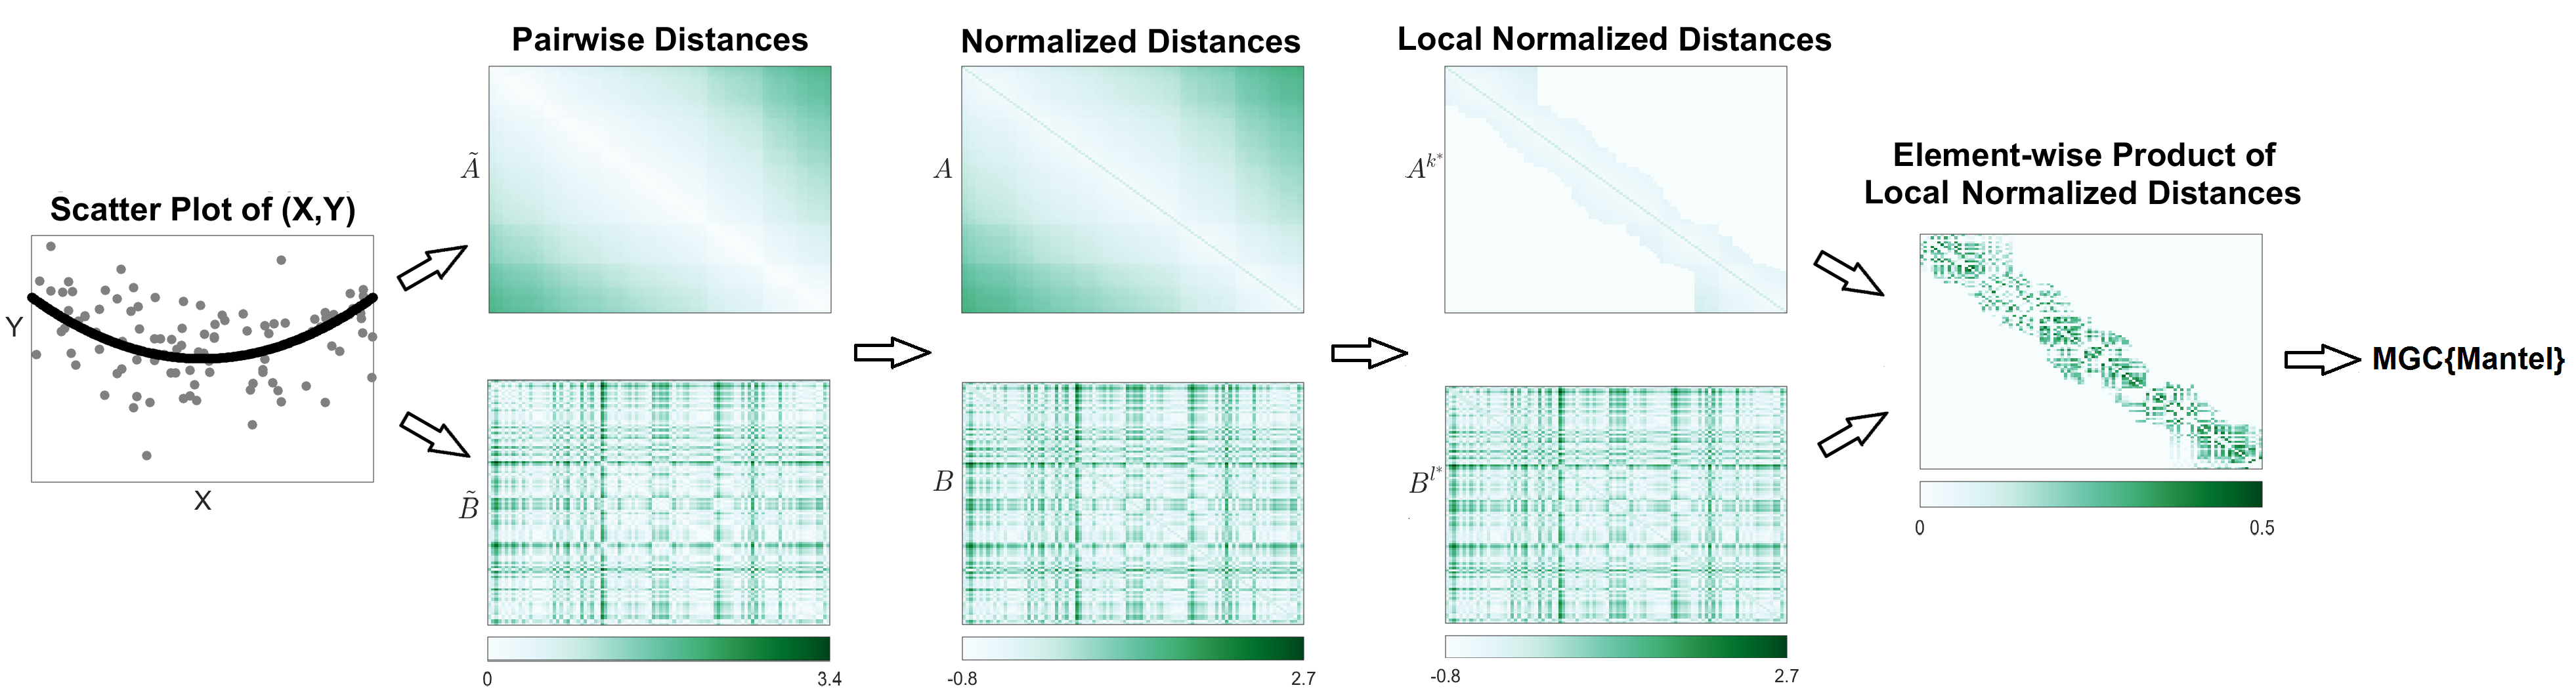
\includegraphics[width=1.0\textwidth]{../Figures/FigC}
\caption{
Flowchart for \Mgc~computation:
Column 1: $(X,Y)$ have a circle relationship.
Column 2: The heat maps of $\tilde{A}$ and $\tilde{B}$, which are the pairwise Euclidean distance matrices of $X$ and $Y$. All distance entries are non-negative.
Column 3: The top and bottom panels are the heat maps of $A=\{a_{ij}\}$ and $B=\{b_{ij}\}$, which are the properly centered distance matrices of $\tilde{A}$ and $\tilde{B}$. The center panel is the heatmap of the entry-wise products of $A$ and $B$, summing over which yields the un-normalized \Mcorr~statistic. As the entries of $A$ and $B$ can be either positive or negative, the entry-wise products can be either positive or negative for nonlinear dependencies, which causes $\Mcorr(X,Y)$ to be close to $0$ and the p-value to be in-significant, as shown in column 5.
Column 4: The top and bottom panels are the heat maps of local $A$ and $B$, i.e., $A^{k^{*}}=\{a^{k^{*}}_{ij}\}$ and $B^{l^{*}}=\{b^{l^{*}}_{ij}\}$, where $(k^{*},l^{*})=(4,4)$ is the optimal scale for the circle relationship. The center panel is the heat map of the entry-wise products of local $A$ and $B$, summing over which yields the un-normalized \Mgc~statistic $\G^{*}$. \Mgc~successfully identifies the optimal local structure for correlation testing, and the resulting entry-wise products are dominantly non-negative, which causes $\Mgc(X,Y)$ to be much larger than $0$ and the p-value to be significant, as shown in column 5.
Column 5: The top panel is the testing powers of all local correlations, where the optimal scale is shown as a dark blue point with many adjacent scales being very close to optimal (light blue points). The bottom panel shows $\Mgc(X,Y)$ and $\Mcorr(X,Y)$ as dark and gray dots on the x-axis, as well as the distribution of the permuted test statistics.}
\label{f:schematic}
\end{figure}
%

Having defined how to compute \Mgc, we face three challenges to make the method practical. First, in addition to the test statistic, we need to compute the null distribution, so that we may find the critical values and p-values.
Second, na\"ively, computing all local $\G^{kl}$ statistics would require an unacceptably large computational budget.
% require $\mc{O}(n^4)$, because it requires $\mc{O}(n^2)$ time to compute each local statistic (Pseudocode \ref{alg:1scale} in Appendix \ref{appen:algorithms}).  That computational burden would be so high as to make doing so impractical.
Third, having computed all local statistics, we require a method for choosing the optimal neighborhood size, in such a way that the test is still consistent, and not biased (so the resultant p-value remains valid).

Computing the p-values from the test statistic is  straightforward.
% , thanks to the advent of permutation testing \cite{GoodPermutationBook}.  
Specifically, we can permute the labels of either the $\mbx_i$'s or the $\mby_i$'s, and then compute the \Mgc~statistics on the permuted data \cite{GoodPermutationBook}.  By permuting the labels, we have rendered the two different views of the data independent.  Doing so many times yields an empirical estimate of the null distribution, which we can use to compute the critical value and p-value. This procedure is somewhat time consuming, which makes computing the test statistics for all neighborhoods efficiently even more important.

 % (see Pseudocode \ref{alg:all_scales} in Appendix \ref{appen:algorithms} for details on our permutation test).


Nearly all algorithms that employ regularization (for example, sparse methods, feature selection, dimensionality reduction) face a similar dilemma: how to efficiently choose the hyper-parameters.
% requires running the entire algorithm again from scratch.
% Unlike many manifold learning methods,
% once the rank information is given,
% 
\jv{Need to discuss the last two paragraphs in this section; and I have combined two running time paragraph into one.}
Most manifold learning algorithms require that the user essentially runs the entire algorithm again from scratch for each different hyper-parameter setting, a pursuit that can be exponentially taxing as the number of hyper-parameters increases.
In our case, once the rank information is provided, each distance-based local correlation takes $O(n^2)$ time to compute (Pseudocode \ref{alg:1scale} in Appendix \ref{appen:algorithms}), which means a straightforward algorithm to compute all local correlations would take $O(n^4)$ time.
% 
However, we have devised an algorithm for exactly computing \emph{all} local correlations in $\mc{O}(n^2 \log n)$, essentially the same running time complexity as  global correlation coefficients (the additional $\log$ factor is for sorting to find the neighbors, see Pseudocode \ref{alg:all_scales} in Appendix \ref{appen:algorithms} for details). We do so by noting that the sufficient statistics for larger neighborhood sizes include those for the smaller sizes, so we can simply keep track of them as we iteratively increase neighborhood size. The end result is \Mgc~can be computed in  time comparable to the other leading dependence tests (see Pseudocode \ref{alg:pval} in Appendix \ref{appen:algorithms} for details on computing all $n^2$ p-values efficiently).
% 
% Therefore, we can efficiently compute all local correlations for a given pair of data and the permuted data, which yields the p-values for each neighborhood size (see Pseudocode \ref{alg:pval} in Appendix \ref{appen:algorithms} for details). But it does not tell us which neighborhood sizes are optimal.

Finally, we must find an optimal scale.
Our procedure for estimating the optimal scale searches for regions of neighborhood sizes for which p-values are consistently low, guarding against noisy scales that appear optimal, and combating bias added by looking at many different scales.
%
The optimal scale is the largest neighborhood size in that region.
The p-value of \Mgc~is therefore the p-value of the optimal scale 
% , and declare significant dependency when the p-value is less than $\alpha$, often $0.05$ 
(see Pseudocode \ref{alg:best_scale} and \ref{alg:power} in Appendix \ref{appen:algorithms} for details).
% By the optimal scale estimation, the \Mgc~statistic $\G^{*}$ is theoretically no worse than the global counterpart $\G$, and usually enjoys better testing powers under high-dimensional and/or nonlinear dependencies; moreover, different \Mgc~implementations may vary slightly in performance depending on the properties of the respective global statistic. In the following sections, we demonstrate that our \Mgc~statistic yields tests that preserve consistency regardless of the functional dependency and dimensionality, improves the testing powers of the respective global correlation under nonlinear and high-dimensional dependencies both in theory and in simulations, as while as being the most superior test in simulations and real data experiments.}



\subsection*{Finite Sample Simulation Experiments}

% From this section onwards, unless mentioned otherwise, our \Mgc~is always implemented for \Mcorr, due to its theoretical consistency and numerical advantages throughout.

% Based on the previous section, we understand \Mgc~can be a consistent tests in a wide variety of settings (all finite dimensional joint distributions with bounded variance)
% %, and those whose dimension increases, respectively).
% But, our theoretical results do not shed light on the finite sample performance of \Mgc.
% %We are interested, therefore, in understand which of these tests performs well in various simulated settings.
% Specifically, 
We are interested in assessing the performance of our newly proposed multiscale tests in a wide variety of settings, to better understand which the tests, and gain insight into which to use in different settings.  
% to previous tests like \Hhg, \Mcorr, \Dcorr, and \Mantel, each of which performs well in a fraction but not all of the simulations.
%\Mcorr~is a generalization of \Dcorr~that achieves better performance in high-dimensional settings, and nearly identical performance in low-dimensional settings, for brevity here. And \Dcorr~is a generalization of \Mantel~that has stronger theoretical support.  Therefore, in this section, we only consider \Mcorr~and \Hhg~as the global benchmarks, and compare them with \Mgcm~(though see Figure \ref{f:nDAll} in Appendix \ref{appen:function} for all algorithm performance).
We therefore consider $20$ different joint distributions $f_{xy}$ corresponding to $20$ different noisy dependence settings. A large fraction of these are taken exactly from existing literature \cite{SzekelyRizzoBakirov2007, SimonTibshirani2012, GorfineHellerHeller2012, HellerGorfine2013}, and we have added several additional settings.  They include
linear and nearly linear  (1-5),
polynomial   (6-12),
trigonometric (13-17),
uncorrelated but nonlinearly dependent  (18-19),
and an independent relationship (20).
Details for each setting are given in Appendix \ref{appen:function}, with a visualization of each dependency shown in Supplementary Figure~\ref{f:dependencies}. For all $20$ settings, we define  $\delta_x$  as Euclidean distance,  $\delta(x_i,x_j) = \sum_{d=1}^{d_x} (x_i(d) - x_j(d))^2$, and the same for $\delta_y$.


\begin{figure}[htbp]
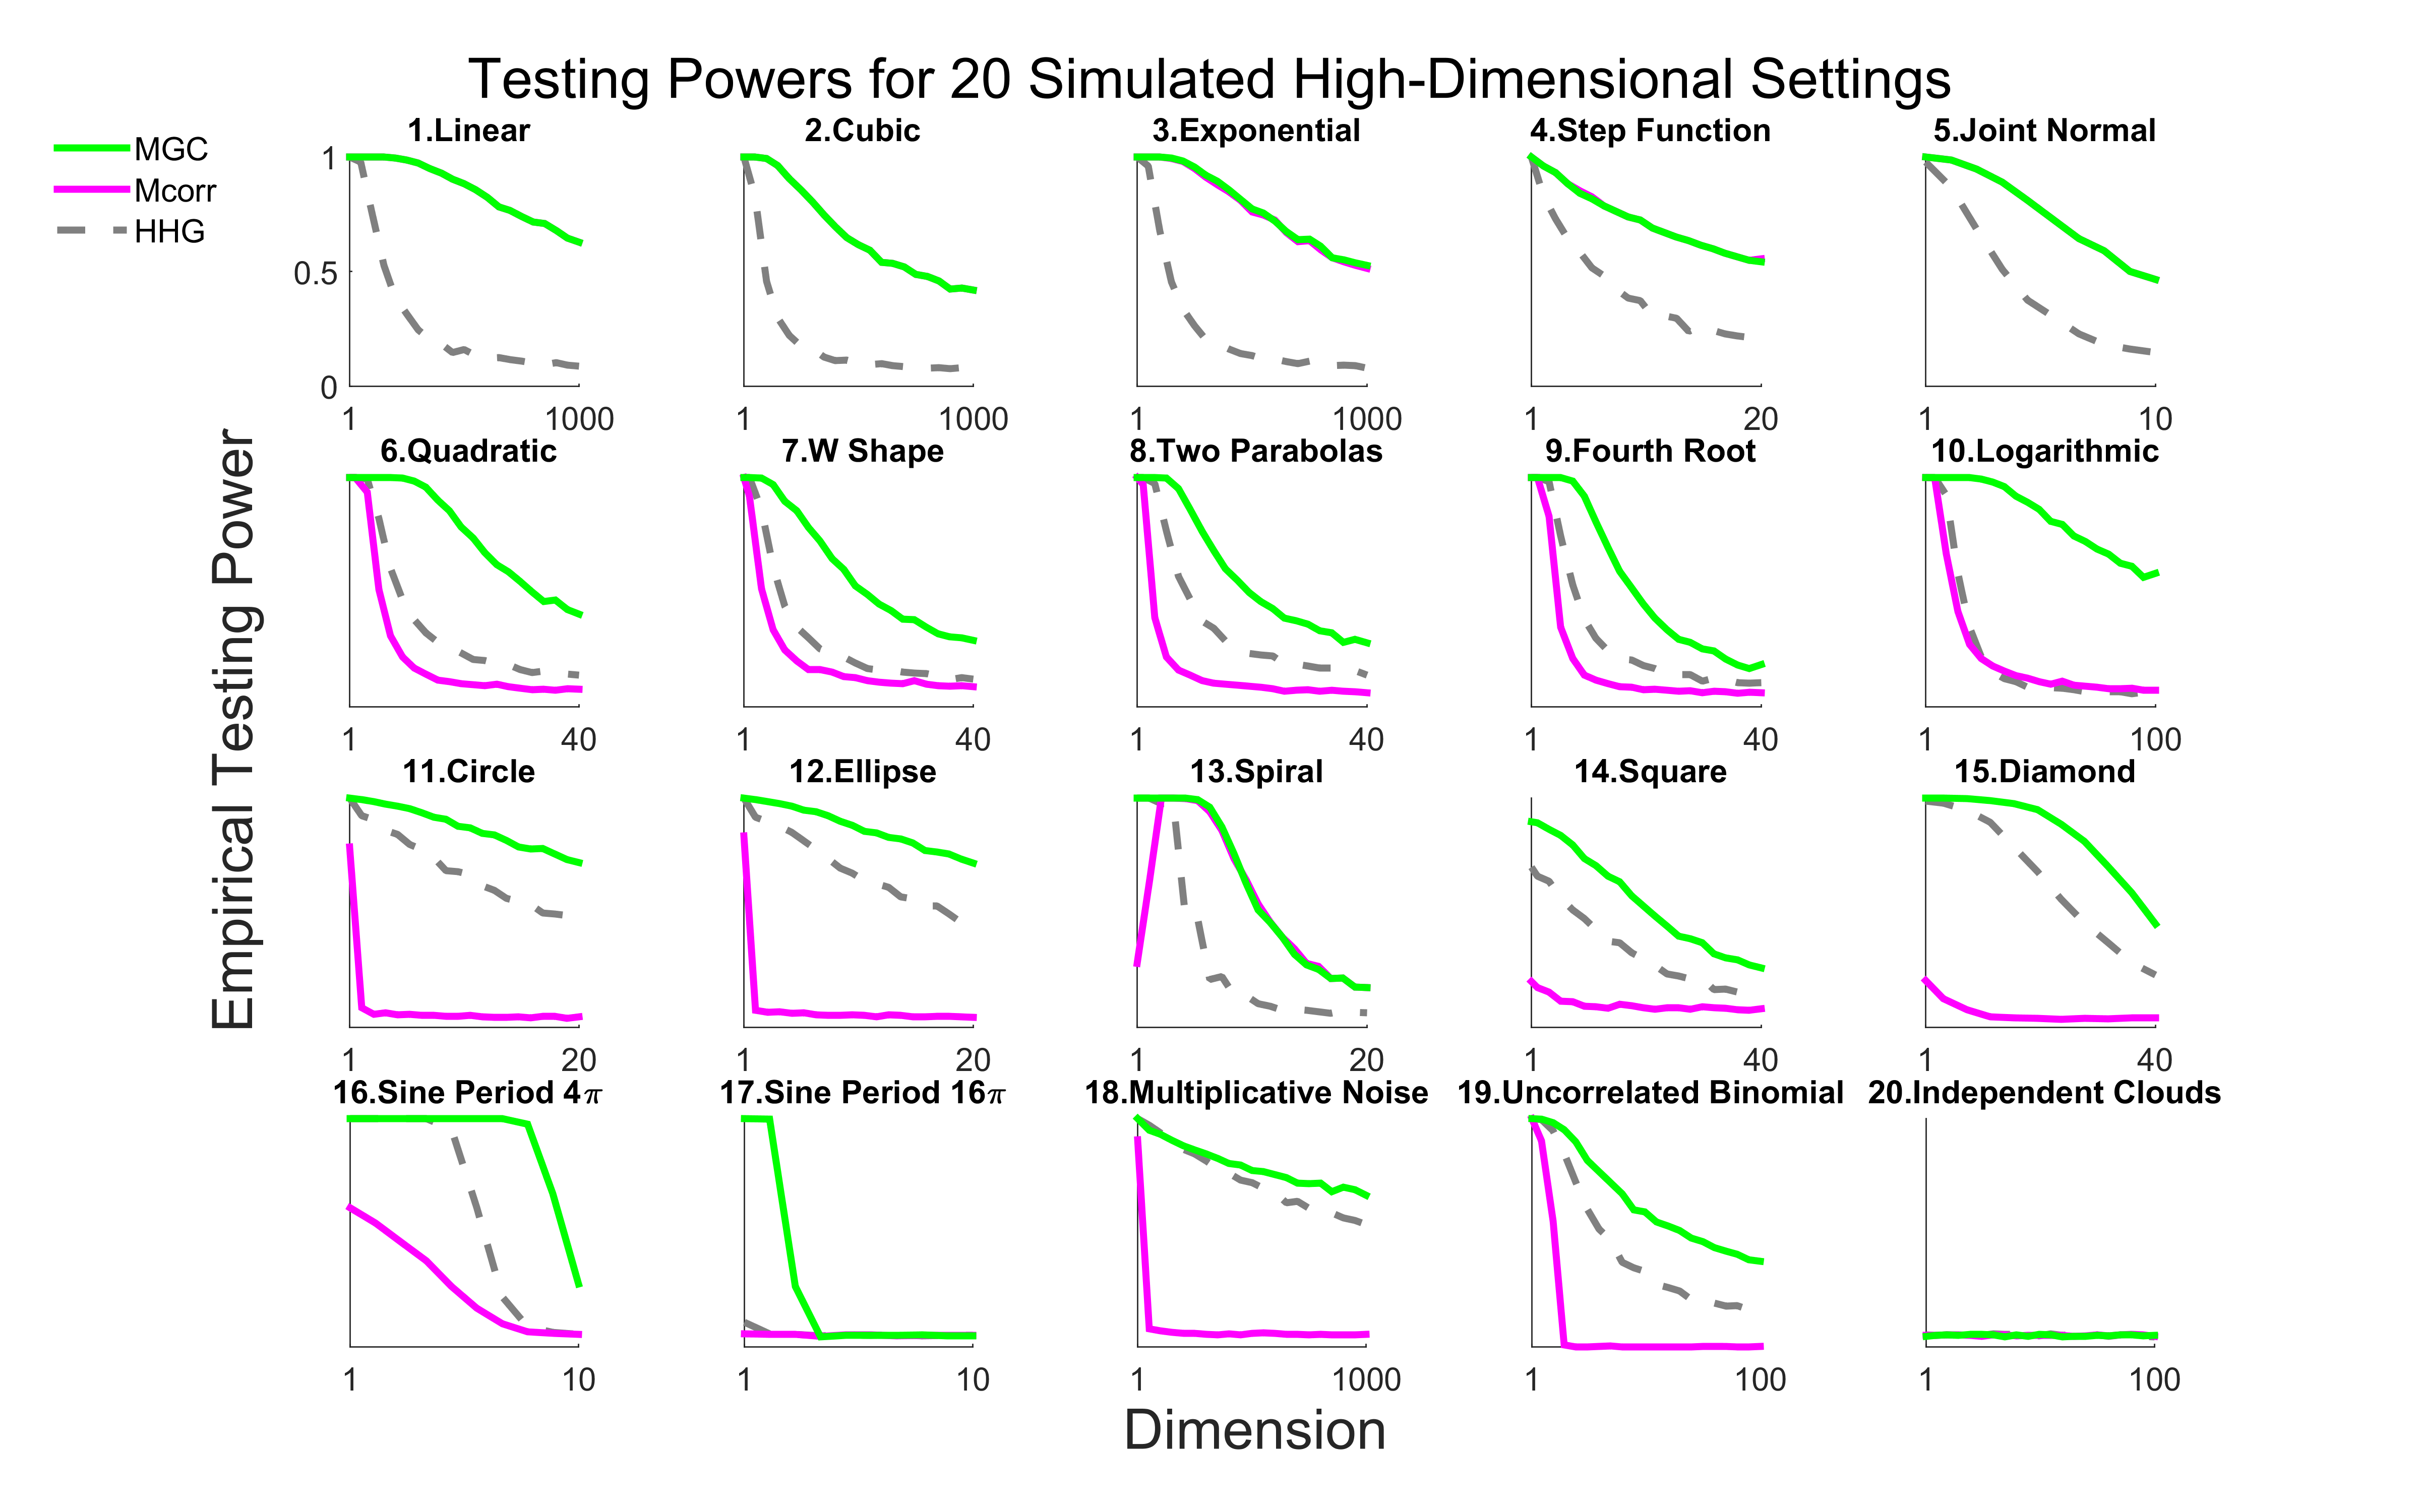
\includegraphics[width=1.0\textwidth]{../Figures/FigHDPower}
\caption{Powers of different methods for $20$ different dependence structures, estimated by the empirical distributions of the test statistics under the null and the alternative on the basis of $10$,$000$ Monte-Carlo replicates. $2$,$000$ additional MC replicates are used for optimal scale estimation for \Mgc.
Each panel shows empirical testing power on the absicca at a significant level $\alpha=0.05$, and the dimensionality on the ordinate.
\Mgc~empirically achieves similar or better power than the previous state of the art approaches for all sample sizes on all problems.
}
\label{f:nD}
\end{figure}


%\subsubsection{Low-Dimensional Simulation Experiments}
%\label{numer1}

%We first experiment on the 20 different $1$-dimensional scenarios, that is, for each scenario, both \mbx~and \mby~are 1-dimensional. To observe how fast the testing power of each method converges to $1$ under each dependency, we plot the testing power as we vary sample size from $5$ to $100$  (Figure~\ref{f:1D}).

%It is immediately clear that in all 20 scenarios for all sample sizes, \Mgcm~performs as well or better than its global counterpart \Mcorr, and this is nearly true comparing \Mgcm~to \Hhg~as well. More specifically, for dependencies that are close to linear (type 1-5), \Mgcm~achieves the same power as \Mcorr~(as it should according to theory), both of which achieve a power as high or higher \Hhg, for all sample sizes.
%For nearly all of the remaining nonlinear dependencies (type 6-19),  \Mgcm~also does as well or better than its global counterparts.  In these settings,  \Mgcm~often performs significantly better than its local counterpart, \Mcorr.
%For the independent clouds,  the empirical power of all the tests, including all \Mgc~tests, are indeed around the type $1$ error level, meaning no false signal is detected.


%\begin{figure}[htbp]
%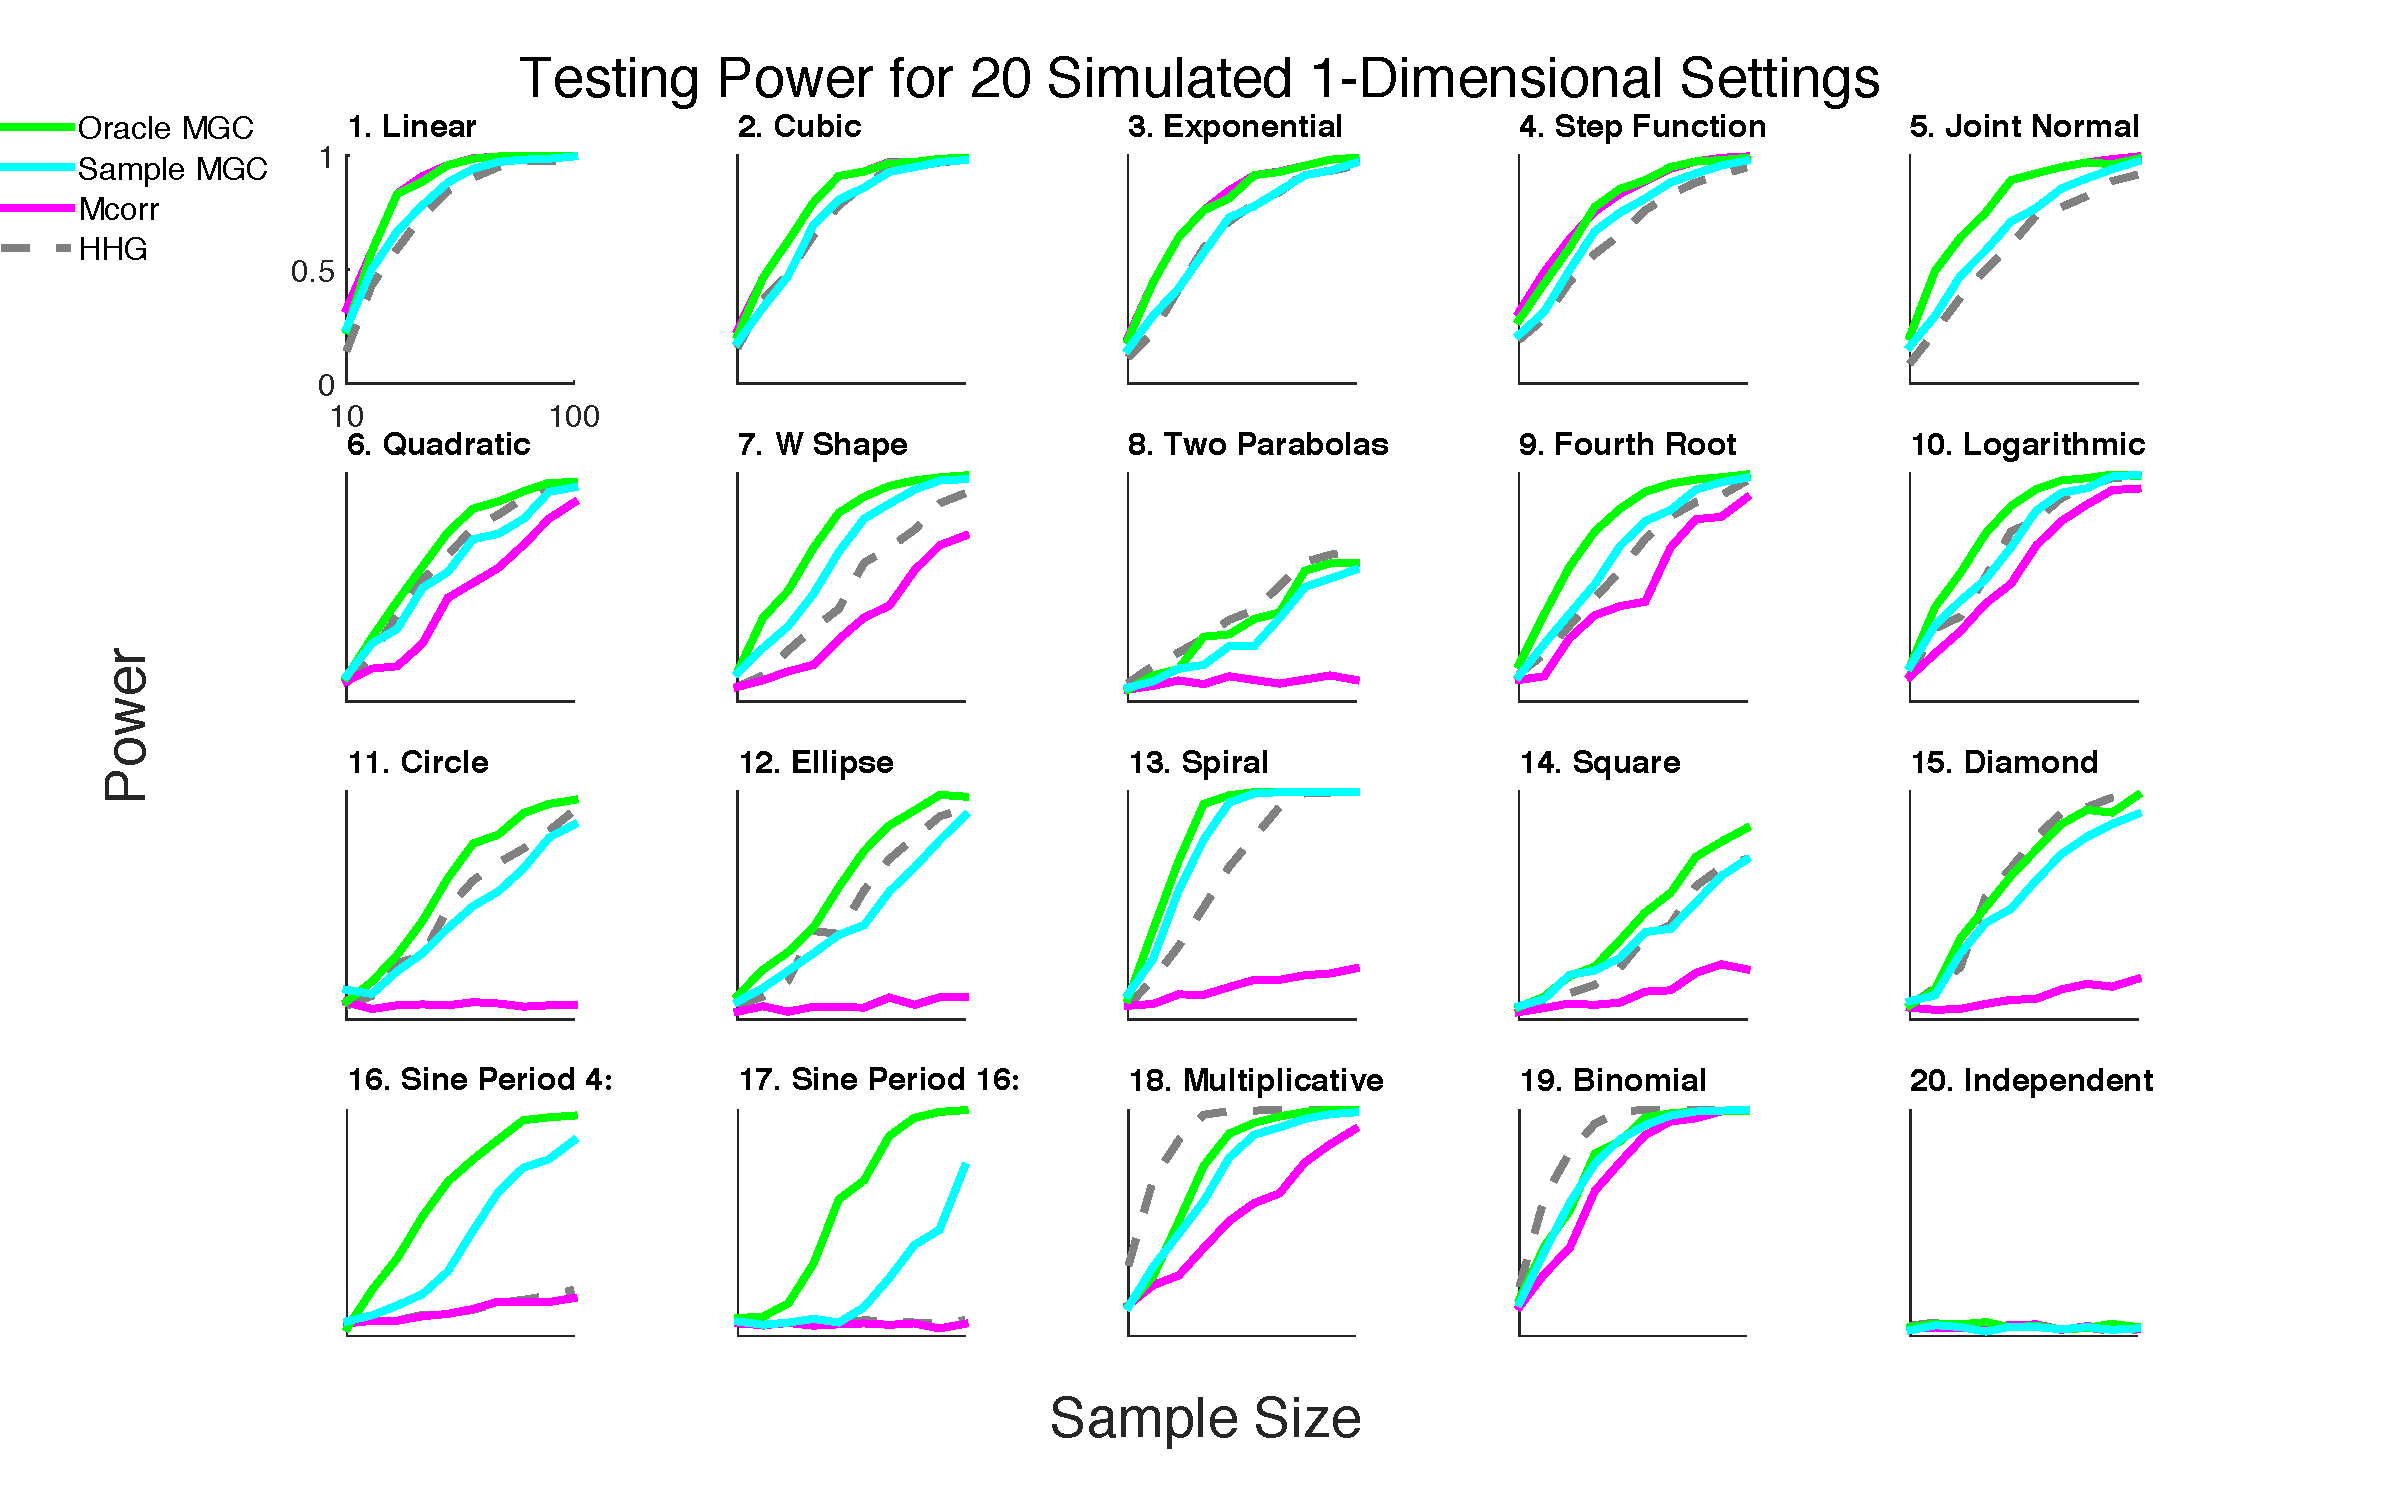
\includegraphics[width=1.0\textwidth]{../Figures/Fig1DPower}
%\caption{
%Powers of different methods for $20$ different $1$-d dependence structures, estimated by the empirical distributions of the test statistics under the null and the alternative on the basis of $10$,$000$ Monte-Carlo replicates. $2$,$000$ additional MC replicates are used for optimal scale estimation for \Mgc.
%Each panel shows empirical testing power on the absicca at a significant level $\alpha=0.05$, and sample size on the ordinate.
%\Mgcm~empirically achieves similar or better power than the previous state of the art approaches for all sample sizes on nearly all problems.}
%\label{f:1D}
%\end{figure}


%\subsubsection{High-Dimensional Simulation Experiments}
%\label{numer2}

%In this section we consider the same $20$ functions as in Section~\ref{numer1}, but increase the dimensionality while keeping sample sizes fixed  at $n=100$.
%Note that for all dependencies, the dimensionality of \mbx~is increasing, but the dimensionality of \mby~increases in only a subset of the settings (see Appendix \ref{appen:function} for details).

Figure~\ref{f:nD} shows the testing powers versus the dimensionality of \mbx~(the dimensionality of \mby~increases in only a subset of the settings; see Methods for details), with the sample sizes fixed at $n=100$ for each setting.  We compare  our novel test, \Mgc, with two previously proposed state-of-the-art tests: \Mcorr~\cite{SzekelyRizzo2013a} and \Hhg~\cite{HellerGorfine2013}.  \Hhg~has previously been demonstrated to perform very well on all sorts of nonlinear dependencies, especially in low-dimensional settings, and enjoys strong theoretical guarantees. 
% 
The advantage of \Mgc~over its global counterpart \Mcorr~and \Hhg~is  stark. For the nearly linear settings, \Mgc~and \Mcorr~are essentially identical and significantly better than \Hhg~as the dimension increases.  For the remaining nonlinear dependencies, \Mgc~achieves superior power than \Hhg~and \Mcorr~for \emph{all} functions, often by a significant margin.  For the independent simulation, all tests yield powers at the significance level $\alpha$,  indicating no more false positives than expected according to the theory.
More exhaustive benchmark experiments, including focusing on the one-dimensional scenarios,
in which we also compare to \Mantel~and \Dcorr, 
as well as our novel multiscale variants of both \Mantel~and \Dcorr, 
 are qualitatively similar, and are therefore relegated to Appendix \ref{appen:figs}. 



\subsection*{\Mgc~Emperically Dominates Global Counterparts}

The above results demonstrate that converting \Mcorr, a global generalized correlation coefficient based test, to \Mgc, its multiscale variant, improves (or does not diminish) testing power for all considered settings, regardless of dimensionality.  We wondered, therefore, whether the multiscale variant of other generalized correlation coefficients would be behave similarly.  Specifically we consider the \Mantel~and \Dcorr~tests, in addition to \Mcorr, and for each, develop a multiscale variant (see Appendix \ref{appen:methods} for details). 
% 
Figure \ref{f:pp} show slopegraphs comparing global and multiscale generalized correlation coefficients.  The top row shows for each of the $20$ settings, with both $x$ and $y$ in 1-dimension, the average power as sample size increases.  The bottom row shows the same, but keeping sample size fixed at $n=100$ and increasing dimensionality of $x$.  In all $40$ settings, both low and increasing dimensions, and both fixed and increasing sample sizes, multiscale methods always improve on or stay the same, and never decrease power.  


 % 
% To better summarize the advantages of global versus local, Figure~\ref{f:pp} shows how the powers change from each global correlation to its \Mgc~implementation, for each dependency in Figure~\ref{f:nD}. Indeed, \Mgc~always improves over its global correlation, regardless of the global correlation that is being used. Note that the actual powers for \Dcorr, \Mantel~, and their \Mgc~variants are included in Appendix \ref{appen:function}, where the same conclusion for \Mgc~superiority still hold. We also present in Appendix \ref{appen:function} an additional simulation setting with increasing sample size and fixed dimensionality to observe that the powers of \Mgc~converge to $1$ faster than all the benchmarks for nearly all dependencies.


%\subsubsection{\Mgc~improves finite sample performance of all global generalized correlation coefficient based tests}
\begin{figure}
  \centering
  \begin{tabular}{@{}p{0.3\linewidth}@{\quad}p{0.3\linewidth}@{\quad}p{0.3\linewidth}@{}}
		\subfigimg[width=\linewidth]{}{../Figures/FigHDMcorr} &
		\subfigimg[width=\linewidth]{}{../Figures/FigHDDcorr} &
		\subfigimg[width=\linewidth]{}{../Figures/FigHDMantel}
  \end{tabular}
  \caption{
Average powers slopegraphs comparing global and \Mgc~tests. For each global test,  the left side corresponds to the mean power of each simulation in Figure~\ref{f:nD}, the right side corresponds to the respective \Mgc~mean power. The thin solid line are shown for  6-19, because \Mgc~equals the global correlation for  1-5 and  20. Then the thick solid line summarizes how the overall mean power (including  6-19) changes from global to \Mgc.
It is clear that \Mgc always significantly improves over its global counterpart.}
\label{f:pp}
\end{figure}

%From Figure~\ref{f:pp}(A)(B), \Mgc~is clearly more reliable than all benchmarks throughout the $1$-dimensional simulations regardless of the actual implementation. \Hhg~is slightly better than \Dcorr~/ \Mcorr~in the performance profiles, because there are more nonlinear simulations than linear in the $20$ dependencies, and \Hhg~has a larger advantage for nonlinear dependency than its disadvantage in linear dependency; the global \Mantel~test has the lowest performance profile, but utilizing local correlations makes \Mgcp~perform similarly as the other two \Mgc~implementations.




% 31 lines; target = 64
\subsection*{Discovery of Dependency Across Scales}
\label{main3}

A multiscale power map is a heatmap of powers for all neighborhood sizes, for a given joint distribution and sample size.
Figure~\ref{f:powermaps} provides the multiscale power maps for all 20 different scenarios for different dimensionalities, illustrating how the powers of local correlations change with respect to increasing neighborhood sizes.
The dimension was chosen as the largest one for which $\Mgc$'s power exceeded 0.5, chosen to highlight the differences between scales.
% , for the high-dimensional simulations
%(the $1$-dimensional case is provided in Figure \ref{f:powermaps1} in Appendix \ref{appen:methods}).
% They are plotted at a fixed sample size and a fixed dimension by the same power thresholds as in Figure~\ref{fig:pp}A and C.

The multiscale power map sheds light into the intrinsic dependency structure.
For nearly linear dependencies (1-5), the best neighborhood choice is always the largest scale, i.e., $k=l=n$. For all strongly nonlinear dependencies (6-19), \Mgc~almost always chooses a smaller scale for $x$ or $y$.
 % in a distribution dependent fashion. 
 Furthermore, similar dependencies have similar local correlation structure, and thus similar optimal scales. For example, quadratic (6) and W (7) are both polynomials of degree 2 with different coefficients, and their power maps are quite similar to each other. Similarly,  (16) and (17) are the same trigonometry function (sine) with different periods, and they share a narrow range of significant local correlations.
Both circle (11) and eclipse (12), as well as square (14) and diamond (15), are closely related functions, and have similar multiscale power maps.
Note that for almost all simulations, there exist a large portion of adjacent local neighborhoods that are equally significant, which is an important observation that we use to approximate the optimal \Mgc~scale for real data.

\begin{figure}[htbp]
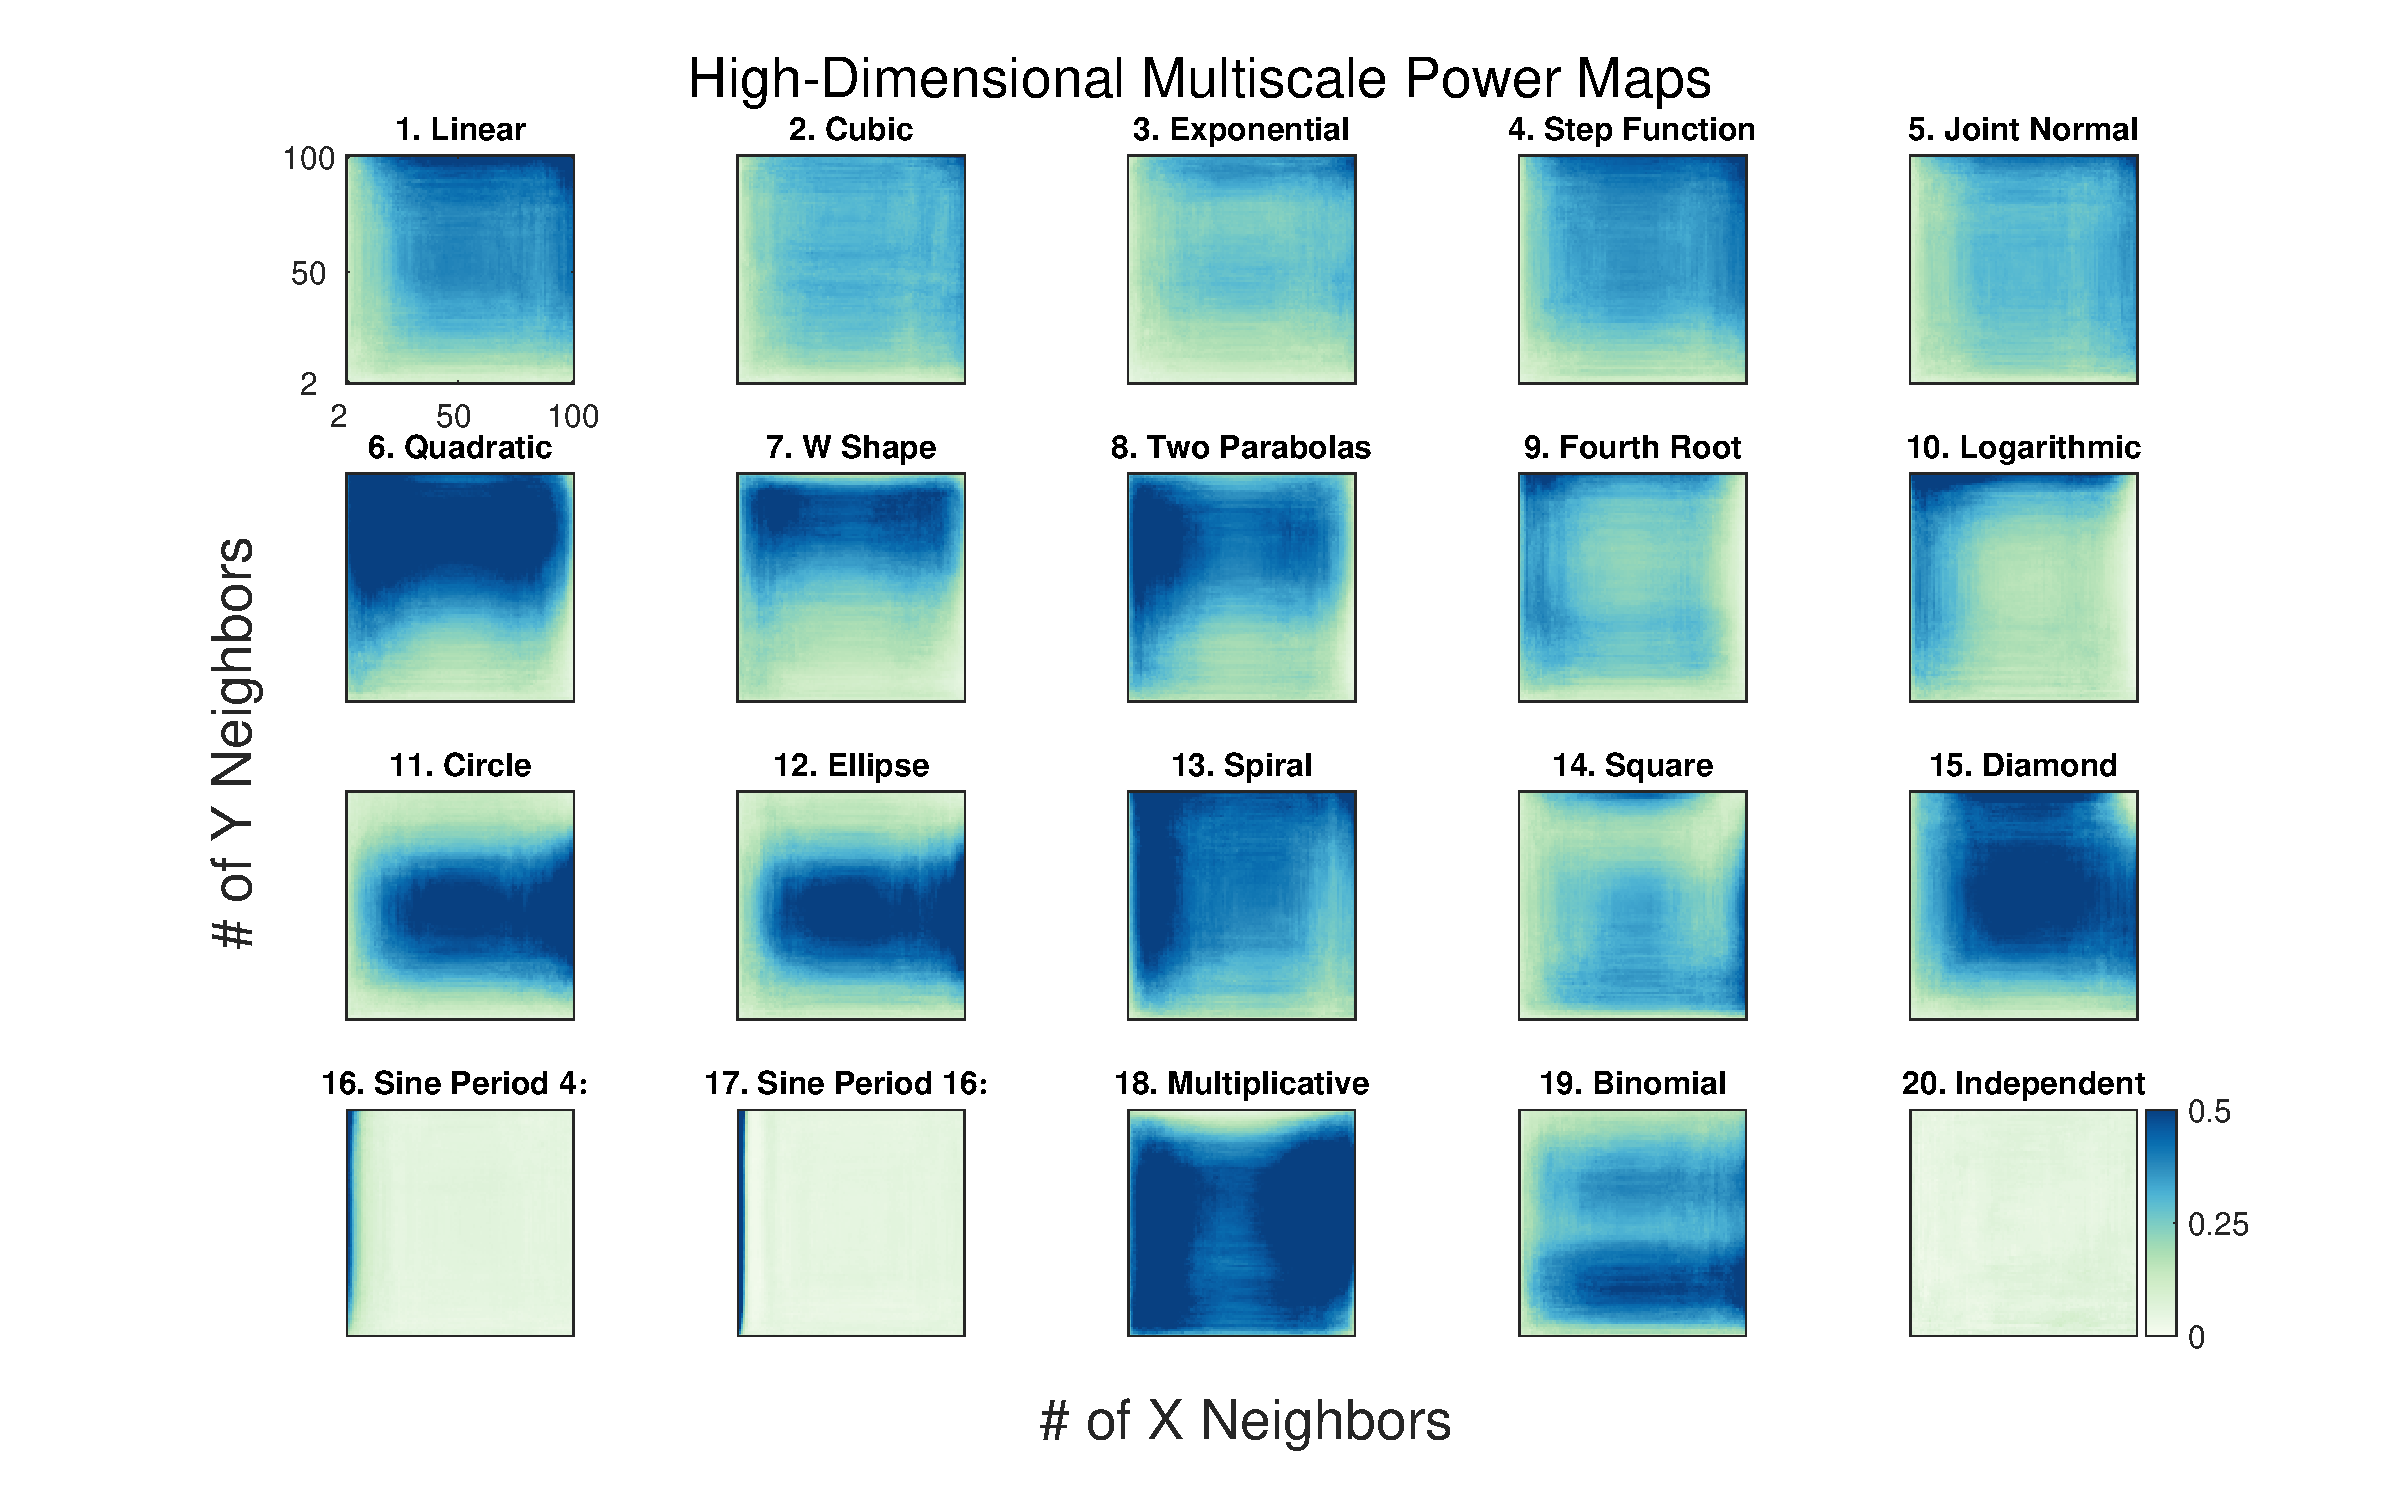
\includegraphics[width=1.0\textwidth]{../Figures/FigHDHeat}
\caption{Influence of neighborhood size on testing power of local correlations at $\alpha=0.05$.
For each of the 20 panels, the abscissa denotes the number of neighbors for $X$ (the scale increases from left to right), and the ordinate denotes the number of neighbors for $Y$ (the scale increases from bottom to top). For each simulation, the sample size is $n=100$, and the dimension is determined by the largest dimension for \Mgc~to have powers exceeding the threshold $0.5$. Each different simulation yields a different surface, highlighting the importance of understanding local scale in terms of understanding the data. }
\label{f:powermaps}
\end{figure}


\subsection*{\Mgc~Theoretically Dominates its Global Counterparts}
\label{s:theory}

The formal testing scenario is as follows: we observe $n$ pairs of observations, $(\mbx_i,\mby_i)$, and we desire to know whether the \mbx's are independent of the \mby's.  To cast this problem as a statistical inference query requires specifying a statistical model, that is, a collection of possible distributions from which we may assume the data arise.  To make the investigation as general as possible, we consider the largest possible set of distributions: any possible joint distribution $f_{xy}$. If \mbx~and \mby~were independent, then it would follow that $f_{xy}=f_x f_y$; in other words, for independent data, the joint distribution is equal to the product of the marginals.  Therefore, we have the following hypothesis testing scenario:
% suppose two data sets $X=[\mbx_{1},\cdots, \mbx_{n}] \in \Real^{d_{x} \times n}$ and $Y=[\mby_{1},\cdots, \mby_{n}] \in \Real^{d_{y} \times n}$ are given, where $n$ is the sample size, $d_{x}$ and $d_{y}$ are the dimensions of each data set. Under the classical hypothesis testing framework, $\mbx_{i}, i=1,\ldots,n$ are assumed identically independently distributed (iid) as $\mb{x} \sim f_{x}$, where $f_{x}$ denotes the distribution of the random variable $\mb{x}$; similarly $\mby_{i}$ are independent realizations of $\mb{y} \sim f_{y}$. Then the null and the alternative hypothesis for testing independence are
\begin{align*}
& H_{0}: f_{xy}=f_{x}f_{y},\\
& H_{A}: f_{xy} \neq f_{x}f_{y}.
\end{align*}
% where $f_{xy}$ denotes the joint distribution of $(\mb{x},\mb{y})$.

The power of a test is defined as the probability that it correctly rejects the null when the null is indeed false.  As defined above, a test is consistent if its power converges to $1$ as sample size increases.
Let $\G_t$ denote a global generalized correlation coefficient based test, that is, $t$ might indicate \Mantel, \Dcorr, or \Mcorr, and let $\beta(\G_t^*)$ denote the power of the corresponding multiscale version.
Recall from the work Szekeley et al. that \Dcorr~and \Mcorr~are both consistent tests. More specifically, \Dcorr~is consistent whenever $f_{xy}$ has finite dimension and bounded variance, and \Mcorr~is consistent even as dimension increases to infinity.  Denote the set of distributions satisfying consistency for a given test by $\mc{F}_t$, where $t$ indicates which test we are referring to. Then, we have the following theorem:
 % in different scenarios, leads us to our first theorem.
% A consistent test statistic has power $1$ asymptotically, i.e., the test statistic under the alternative is asymptotically larger than the statistic under the null. Denote the type 1 error level as $\alpha$, the testing power of \Mgc~as $\beta_{\alpha}(\G^{*})$, and the power of the respective global test as $\beta_{\alpha}(\G)$. Assuming the optimal scale is estimated by the testing power, we have the following theorem regarding the consistency of \Mgc, whose proof is provided in Appendix \ref{appen:proofs}:
\begin{thm}
\label{thm1}
$\beta(\G_t^*) \rightarrow 1$ for all $f_{xy}$ in $\mc{F}_t$.
% whenever $\beta(\G)$ does.
% Suppose for given $f_{xy}$ and $\alpha$, $\beta_{\alpha}(\G) \rightarrow 1$ as $n \rightarrow \infty$, then $\beta_{\alpha}(\G^{*}) \rightarrow 1$ as well.
\end{thm}

Therefore, \Mgc~is consistent against all dependent alternatives for which its global counterpart is. 
% Asymptotic consistency, however, does not convey to us how quickly \Mgc~achieves optimal power in various settings, and whether it exhibits significant advantage over its global counterpart and other popular methods.  For that, we turn to numerical simulations.

For finite samples, however, things appear more interesting.
% The above described qualitative descriptions led us to believe the following two conjectures.  
For linear dependencies,  the optimal \Mgc~scale was empirically always the global one. We therefore conjectured and proved the following:
\begin{thm}
\label{t:linear}
If $\mb{x}$ is linearly dependent on $\mb{y}$, then for any $n$ it always holds that
\begin{equation}
\beta(\G^{nn}) = \beta(\G^{*}) = \beta(\G).
\end{equation}
Thus the optimal scale for \Mgc~is the global scale for linearly dependent data.
\end{thm}


Second, under certain nonlinear dependencies, \Mgc~can achieve a better finite-sample testing power than its corresponding global correlation. Indeed, we were able to prove both of these claims:


On the other hand, for finite sample nonlinear dependencies (which better characterize all real data), we note that \Mgc~almost always \emph{improves} upon its global counterpart.  We therefore conjectured and proved the following:
\begin{thm}
\label{t:non}
There exists $f_{xy}$ and $n$ such that
\begin{equation}
\beta(\G^{*}) > \beta(\G).
\end{equation}

Thus multiscale graph correlation can be better than its global correlation coefficient under certain nonlinear dependency, for finite sample.
\end{thm}
Note that Theorem~\ref{t:linear} and Theorem~\ref{t:non} hold for any of \Mgc~varieties, including  \Dcorr, \Mcorr, and \Mantel.
%
The proofs of Theorem~\ref{t:linear} and \ref{t:non} are both in Appendix \ref{appen:proofs}.  The proof of Theorem~\ref{t:linear} is straightforward.  The proof of Theorem~\ref{t:non} is a constructive one. More specifically, we constructed quadratic function and sampled data a finite number of times and exactly compute the power for both \Mgc~and \Dcorr, proving that \Mgc~has higher power in this setting. This shows that \Mgc~can outperform its global counterpart even for the most modest nonlinear functions.  Because any function can be approximated by a polynomial expansion \cite{RudinBook}, the proof of Theorem~\ref{t:non} suggests that \Mgc~is able to outperform its corresponding global correlation on a wide variety of nonlinear functions, which is indeed the case throughout the numerical simulations. To our knowledge, Theorems \ref{t:linear} and \ref{t:non} are the first finite sample theorems for dependence testing.
\cs{is that true?}

The three above theorems taken together lead to the main theoretical result of this manuscript:
\begin{thm}
\Mgc~dominates its global counterpart, meaning that \Mgc~is always as good as, and sometimes better than, its corresponding global correlation coefficient. 
\end{thm}


%\subsection*{Robustness against Outliers}
%\label{s:outliers}

%Above we demonstrated via theory and simulations that \Mgc~works well in a wide variety of settings, but all of the previously mentioned settings lacked outliers, that is, points that are not dependent.  Because real data quite often includes outliers, for \Mgc~to be useful in practice, it is important to be robust to them.
%To study the outlier regime, we consider the following  simple mixture model: the joint distribution is a mixture of two components, a dependent component and an independent component.  We can therefore control the fraction of outliers by varying the relative weights of the two components.

%Figure \ref{f:outliers} shows an illustrative example.  Specifically, we generate data from the following distribution:
%\begin{equation} \label{e:outlier}
%f_{xy}=w f_{1}+(1-w) f_{2}, \text{ where } f_{m} \sim \mc{N}(\mu_{m},\Sigma_{m}),
%\end{equation}
 % and $f_{2} \sim \mc{N}(\mu_{2},\Sigma_{2})$.
%and we set $\mu_{1}=(0,0)$, $\mu_{2}=(5,-5)$, $\Sigma_{1}$ is a matrix with ones on the diagonal and $0.9$ elsewhere,
% $ = \mb{1}\T\mb{1}$, $\begin{bmatrix} 1&1\\ 1&1 \end{bmatrix}$,
 %and $\Sigma_{2}$ is the identity matrix (ones on the diagonal and zero elsewhere).
 % $ = \begin{bmatrix} 1&0\\ 0&1 \end{bmatrix}$.
 %The above mixture implies that \mbx~and \mby~are  linearly correlated with probably $w$, and \mbx~and \mby~are independent with probability $(1-w)$.
%The top row of Figure~\ref{f:outliers} shows exemplar datasets with 30\%, 50\%, and 70\% outliers; the bottom row shows the multiscale power maps for each.
% at each $w$ by the same procedure as in section~\ref{numer1}.

%A few points are evident from the figure.  First, \Mgc~achieves a much higher power than its global counterpart  \Mcorr~(evidenced by considering the power of \Mgc$^{n,n}$ in each panel, and noticing that it has much lower power than the maximum of each power map), regardless of the fraction of outliers. \Mgc~is also better than \Hhg: the power of \Hhg~is $1, 0.75,0$ at $w=0.7,0.5,0.3$ respectively, which drastically decreases as $w$ decreases, while \Mgc~always maintains power $1$.
%Furthermore, \Mgc~provides useful information regarding the fraction of outliers: the optimal scale $(k^{*},l^{*})$ is directly related to the mixture probability $w$, specifically $k^{*}=l^{*}=\min(wn,(1-w)n)-1$ is always optimal. Intuitively, \Mgc~is robust against outliers because the optimal local scale automatically excludes the independent outliers from the dependent observations in testing. The robustness still holds as the dimension, sample size, or the underlying dependency changes (not shown).

%\begin{figure}
 % \begin{tabular}{@{}p{0.3\linewidth}@{\quad}p{0.3\linewidth}@{\quad}p{0.3\linewidth}@{}}
  %  \subfigimg[width=\linewidth]{}{../Figures/FigOutlierVisual1} &
   % \subfigimg[width=\linewidth]{}{../Figures/FigOutlierVisual2} &
    %\subfigimg[width=\linewidth]{}{../Figures/FigOutlierVisual3} \\
    %\subfigimg[width=\linewidth]{}{../Figures/FigOutlierPower1} &
    %\subfigimg[width=\linewidth]{}{../Figures/FigOutlierPower2} &
    %\subfigimg[width=\linewidth]{}{../Figures/FigOutlierPower3}
  %\end{tabular}
  %\caption{\Mgc~is robust against outliers. We simulated $n=100$ data points  according to  Equation \eqref{e:outlier} with 30\%, 50\%, and 70\%  outliers (depicted across the three columns).
  %Top row shows scatter plots of an exemplary dataset, the bottom row shows multiscale power maps at critical level $\alpha=0.05$.  It is evident that
 %  samples under the outlier model in the main text, with different fractions of outliers in the three columns.  The bottom row shows the
	% (A) Scatter plot of samples $(X,Y)$ under the outlier model with probability $w=0.3$. Black points are dependent data, while the gray points are independent outliers.
	% (B) Same as $A$ with $w=0.5$.
	% (C) Same as $A$ with $w=0.7$.
	% (D) Influence of neighborhood size on testing power of local correlations, under the outlier model with probability $w=0.3$.
	% (E) Same as $D$ with $w=0.5$.
	% (F) Same as $D$ with $w=0.7$.
%\Mgc~is always better than global \Mcorr, and the optimal scale informs us as to the fraction of outliers.}
%\label{f:outliers}
%\end{figure}

\subsection*{Real Data Experiments}
\label{numer3}

\subsubsection*{Only Local Scales can Detect Dependence} % Between Hippocampus Shape and Depression}

Our first real data experiment investigates whether brain shape and disease status are  dependent on one another.  Previous investigations have linked major depressive disorder to the hippocampus shape \cite{ParkEtAl2008,PosenerEtAl2003}, though global tests were unable to detect a statistically significant dependence structure at the $\alpha=0.05$ level.

 % for both hemispheres.
% The first experiment is to test dependency between the brain hippocampus shape and major depressive disorder.

This brain shape versus disease dataset consists of $n=114$ subjects, for each we have an MRI scan as well as a categorical variable indicating whether the subject is clinically depressed, high-risk, or non-affected.  From the MRI data, previous work  extracted both the left and right hippocampi.   For the brain shape ``view'' of the data, they computed the interpoint comparison matrices using a nonlinear landmark matching approach \cite{ParkEtAl2008,BegEtAl2005}.
% To start with, we transform the respective data sets into dissimilarity matrices: for the brain data, two dissimilarity matrices representing the left and right hippocampus data are obtained based on landmark
% matching (see \cite{ParkEtAl2011} for more details on data processing);
For the categorical disorder variable,
we use squared Euclidean distance, then add $1$ to every non-diagonal entry (so only the diagonals are of distance $0$). \cs{make sure the above is correct.}

We consider two dependence tests, one for each hemisphere: is hippomcapus shape independent of depressive state.
% testing dependency between the left brain and major depressive disorder, and testing dependency between the right brain and major depressive disorder.
% The resulting p-values based on $r=10$,$000$ random permutations are reported in the first two rows of Table~\ref{table1}. For testing between the left brain and the disorder, \Mgc~/ \Hhg~/ \Mantel~yield significant p-values with \Dcorr~/ \Mcorr~being slightly higher than significance; for testing between the right brain and the disorder, only \Mgc~yields significant p-value, and all benchmarks have p-values higher than significance.
Figure \ref{f:real}A provides the p-value curves for \Mgc~for $k=2,\ldots,n$ at $l=4$  (we only show $l=4$ because the other curves look similar). Many local scales yield significant p-values (around $0.01$) for both hemispheres, whereas the global scale does not detect a significant dependence in either hemisphere. None of the previously proposed dependence tests under consideration (\Mantel, \Dcorr, \Mcorr, or \Hhg) were able to detect dependence for both hemispheres (not shown).
% , which is the reason that \Mgc~can successfully identify the signals in both tests, and implies a similar local dependency structure.


% \begin{table*}[!t]
% \caption{The p-values by the permutation test, for testing dependence on $4$ different pairs of real data. Significant p-values are highlighted. \Mgc~is able to consistently identify significant relationship for the first three rows, and does not inflate the p-value in the last row.
% % \Large
% \renewcommand{\arraystretch}{0.5}
% \centering
% {\begin{tabular}{|c||c|c|c|c|c|c|c|}
% \hline
% Testing Method & \Mgc~& \Dcorr~& \Mcorr~& \Mantel~& \Hhg~\\
% \hline
% Left Brain vs Disorder  & $\textbf{0.0046}$ & $0.0745$ & $0.0783$ & $\textbf{0.0382}$ & $\textbf{0.0375}$ \\
% \hline
% Right Brain vs Disorder & $\textbf{0.0133}$ & $0.1046$ & $0.1104$  & $0.0848$ & $0.0809$\\
% \hline
% \Migraine~vs CCI & $\textbf{0.0111}$ & $\textbf{0.0088}$ & $\textbf{0.0111}$  & $\textbf{0.0093}$ & $\textbf{0.0341}$\\
% \hline
% % \mtg~vs CCI & $0.0712$ & $0.0682$ & $0.0712$  & $0.3314$ & $0.6553$\\
% % \hline
% \end{tabular}
% \label{table1}
% }
% \end{table*}

\begin{figure}
  \centering
  \begin{tabular}{@{}p{0.3\linewidth}@{\quad}p{0.3\linewidth}@{\quad}p{0.3\linewidth}@{}}
	  \centering
    \subfigimg[width=\linewidth]{A}{../Figures/FigReal1} &
    \subfigimg[width=\linewidth]{B}{../Figures/FigReal3} &
    \subfigimg[width=\linewidth]{C}{../Figures/FigRealCORR}
  \end{tabular}
\caption{
(A) Local correlation p-value curves with respect to $k=2,\ldots,114$ at $l=4$ for brain vs disease. Dark lines correspond to the largest region of significant scales.
(B) Local correlation p-value heat map with respect to $k=2,\ldots,109$ and $l=2,\ldots,38$ for brain \Migraine~vs CCI.
(C) Density estimate for the false positive rates of \Mgc~on the brain vs noise experiments, with the actual rate of each data shown as dots above the x-axis.}
\label{f:real}
\end{figure}

\subsubsection*{\Mgc~can provide insight into the nature of the dependence structure}
% : Brain Structural Network vs. Personality}

The next real data experiment investigates whether brain networks and personalities are independent of one another. Previous work \cite{AdelsteinEtAl2011} investigated whether individual voxels were related to specific dimensions of personality, but were unable to compare entire brain networks to a higher-dimensional characterization of personality. 
In this dataset, we have $n=XXX$ subjects, for each we obtained a resting-state functional MRI scan as well as her five-factor personality trait as quantified by  the NEO Personality Inventory-Revised  \cite{Costa1992}. \cs{how many subjects? which atlas did we use? how did we represent the data? what metric did we use for each view? etc.}  

 Figure \ref{f:real}B shows that  global dependence tests can ascertain whether the whole brain-network is independent of the subject's personality.  However, the global test is quite fragile, even ignoring a single subject from the global test can render the test non-significant.  On the other hand, \Mgc~is more robust, there is a whole region of neighborhood sizes such that the test is quite significant.  Moreover, that the local tests performs optimally with approximately 30 neighbors suggests that these data have multiple cohorts, for which the dependence structure likely differs.  This result therefore suggests  the next investigatory steps to take to further understand the nature of the dependence structure between brain networks and personality.



% Next we experiment on \Migraine~vs CCI and \mtg~vs CCI. More specifically, we estimated brain graphs from diffusion MRI data using two different pipelines, one called \Migraine, and the other called \mtg.  The question we have is whether brain graphs are independent of personality.  Because we cannot directly measure brain graphs, we must estimate them from the data.  Currently, the jury is out on which estimation procedure is best.  Therefore, we tried two different brain-graph estimation pipelines to determine which worked better for this particular task.

% Using the same testing procedure as the previous experiment, the resulting p-values for \Migraine~vs CCI and \mtg~vs CCI are reported in the last two rows of Table~\ref{table1}. The dependency between \Migraine~and CCI is strong enough for all dependence tests to return significant p-values; in particular, we observe that there exists many local scales with significant p-values for \Migraine~vs CCI from the p-value heat map in Figure~\ref{f:real}(B). But there appears to be a loss of dependency between \mtg~and CCI, as most significant scales for \Migraine are no longer significant when testing on \mtg. (The p-value heat map for \mtg vs CCI is not shown, as it has no significant scale.)

% All the benchmarks also suggest the disappearance of significant dependency, but they do not exhibit the local structure difference. And \Mantel~and \Hhg~are less informative due to the large change of p-values when moving from \Migraine~to \mtg. Note that if we test independence between \Migraine~vs \mtg, the p-values of all tests are $0$, indicating a strong dependency.

% Therefore in this exploration task, \Migraine~is a better brain graph estimator than \mtg: although they are strongly related with each other, \Migraine~is more dependent with CCI than \mtg, because \mtg~is a transformation of \Migraine~without consideration of CCI. Our method identifies the better representation of the two, reveals the local dependency loss from the p-value heat maps, and does not identify false signals. Thus \Mgc~can be used to find the most relevant representation / variable and provide valuable insights into the structural difference.

\subsubsection*{\Mgc~Does Not Inflate False Positive Rates} %: Brain Activity vs. Noise}

In the last experiment, \Mgc~is applied to test independence between brain voxel activities and non-existent stimulus similar to a pair of studies led by Eklund et al. \cite{EklundKnutsson2012,Eklund2015}, by using $26$ resting state fMRI data sets from the 1000 functional connectomes project (\url{http://fcon_1000.projects.nitrc.org/}), consisting of a total of XXX subjects.
\cs{please fix} 
We used CPAC \cite{CPAC2015} to estimate regional time-series, in particular, using the sequence of pre-processing decisions determined to optimize discriminability \cite{Wang2016}.  The output for each scan is the resting state fMRI time-series data containing $200$ regions of interest for $200$ time-steps.
We then also generate an independent stimulus  by sampling from a standard normal at each time step.  Of course, the brain activity data and the stimuli are independent by construction.
For each brain region, we test: is activity of that  brain region independent of the time-varying stimuli. We pool brain activity over all of the samples from the population.
Any regions that are detected significant are false positives by definition.  By testing reach brain region separately, we obtain a distribution of false positive rates.  If our test is unbiased, that distribution should be centered around the critical level, which we set at $0.05$ for this experiment.


To conduct this test, we must construct a distance matrix for brain region activity, and another for the stimulus. For each brain region, we compute $a_{ij}=\|\mbx_{\cdot i}-\mbx_{\cdot j}\|_2^2$, for all $(i,j)$ pairs,  where $\mbx_{\cdot i}$ denotes the observation vector of all subjects at time-step $i$.
For the stimulus, we similarly compute the Euclidean distance between activity at all pairs of time-steps: $b_{ij}= (y_i - y_j)^2$.
\cs{am i right?}
Note that the distance matrices at different brain regions are distinct, but the stimulus is the same for all brain regions during the same experiment.
% From the two distance matrices, we test the dependency between each brain region and the time-varying stimulus by \Mgc.
% The p-values are based on $1000$ random permutations.

For each data set, the above test is carried out for each brain region, and the false positive rates of \Mgc~for each dataset are shown in Figure~\ref{f:real}C. %The y-axis stands for FPR by log scale, and the x-axis shows the name of the data set arranged by increasing FPR; the mean FPR of \Mgc~is shown as the purple-red straight line, with the type $1$ error level $0.05$ drawn as the blue straight line.
% Because the stimulus is in fact independent of the brain activities, the false positive rate should be close to $\alpha=0.05$ for each data set.
\Mgc~false positive rate is centered around the critical level $0.05$, as it should be.
% ; the mean/standard deviation is $0.060 \pm 0.025$.
In contrast,  standard methods for fMRI analysis, such as generalized linear models, significantly increase  or decrease the false discovery rates, depending on the data \cite{EklundKnutsson2012,Eklund2015}.

\subsection*{Discussion}
\label{conclu}

We propose multiscale graph correlation to test independence between measurement types.
We demonstrate via simulations that \Mgc~empirically performs well in linear and non-linear settings, regardless of the dimension, sample size, and noise statistics.  Moreover, it efficiently adapts to the data, to provide not just a valid p-value, but also a picture of which scales contain the dependence structure. We then prove that it dominates global generalized correlation coefficients in finite samples, the first finite sample theorems for dependence testing that we are aware of.  
 % achieves optimal power asymptotically no matter what the dependence structure is.  
In real data experiments \Mgc~reveals dependence where global methods fail, discovers the scale of dependence where global methods succeeded, and did not falsely detect signals when there were none.



A method closely related to distance correlation tests arises from the machine learning community: kernel-based independence test  \cite{GrettonEtAl2005, GrettonGyorfi2010, GrettonEtAl2012}.  Recent work has demonstrated the equivalence between these kernel tests and the energy statistics work \cite{SejdinovicEtAl2013, RamdasEtAl2015}. Thus, we may be able to glean further insights by casting \Mgc~within the kernel framework. Specifically, more efficient tests using asymptotic null distribution approximations are possibly available.

Two other tests merit particular mention at this point.  First, Dumcke et al \cite{Dumcke2014} recently proposed a related nearest-neighbor based test.  Unfortunately, their proposed test requires estimating relative high-dimensional densities, and therefore, does not perform particularly well, nor does it have strong theoretical support.
Finally, Reshef et al \cite{Reshef2011} is another dependence testing methodology, but does not perform as well as energy based tests in various benchmarks \cite{SimonTibshirani2012}, and is designed specifically for low-dimensional settings.
% their actual test is an approximation with unknown error bound relative to their theoretical claims.

\cs{maybe we should mention some sparsity something, since we are sparsifying?}
\jv{not sure what you mean above, let us talk}
\cs{i don't know where you are going with the below paragraph, so i removed}
% Although our definition of local correlation coefficient is fast to implement, generally applicable to any global correlation, and achieves good testing powers, there are multiple ways to combine neighborhood information into a particular global correlation coefficient. So it is possible that the testing performance may be further improved, by tailoring a different centering or ranking scheme for a given global correlation, or by coming up with a different rank-truncated pairwise comparison. Overall, a more thorough investigation on the finite-sample performance of \Mgc, its possible extensions, and other existing methods, are much needed in the future to enhance our understanding of dependence discovery.

While in this work we proved that there exist scales that improve upon the global scale, we did not yet prove that the scale we do select is optimal.  Figure \ref{f:simPerm} shows that our estimated scales are accurate


Furthermore, the optimal scale for \Mgc~is also of interest, such as how to more accurately select the local scale under unknown models for a particular inference task, and the implication of the optimal scale on the geometry of underlying dependency, etc. Another direction we are investigating is how to choose the optimal metric for given data. Beyond the dependence testing framework, it may also be promising to pursue the applications of \Mgc~and local correlations in other closely-related subjects, such as dimension reduction, classification, other testing and prediction domains, etc.

\cs{scaling up via FlashX?}

\bibliographystyle{Science}
\bibliography{MGCbib}


\section*{Acknowledgment}
% \addcontentsline{toc}{section}{Acknowledgment}
This work was partially supported by
%
National Security Science and Engineering Faculty Fellowship (NSSEFF),
%
Johns Hopkins University Human Language Technology Center of Excellence (JHU HLT COE),
%
Defense Advanced Research Projects Agency's (DARPA) SIMPLEX program through SPAWAR contract N66001-15-C-4041,
%
and the XDATA program of the Defense Advanced Research Projects Agency (DARPA) administered through Air Force Research Laboratory contract FA8750-12-2-0303. The authors thank Dr. Brett Mensh of Optimize Science for acting as our intellectual consigliere.



\appendix
\setcounter{figure}{0}
\renewcommand\thefigure{A\arabic{figure}}

\section{Simulation Functions}
\label{appen:function}

We list the distributions of the $20$ dependencies used in the simulations, which are based on a combination of the simulations used in \cite{SzekelyRizzoBakirov2007, SimonTibshirani2012, SimonTibshirani2012, GorfineHellerHeller2012} but with some changes (such as the inclusion of additional noise and an extra weight vector) to better compare all methods throughout different dimensions and sample sizes.

For each sample $\mbx \in \Real^{d_{x}}$, we denote $\mbx^{d}, d=1,\ldots,d_{x}$ as the $d$th dimension of \mbx. For the purpose of high-dimensional simulations, $w \in \Real^{d_{x}}$ is a decaying vector with $w^{d}=1/d$ for each $d$, such that $w\T \mbx$ is a $1$-dimensional weighted summation of all dimensions of \mbx, which equals \mbx~if $d_{x}=1$.
Furthermore, $\mc{U}$ denotes the uniform distribution, $\mc{B}$ denotes the Bernoulli distribution, $\mc{N}$ denotes the normal distribution, $u$ and $v$ represent realizations from some auxiliary random variables, $c$ is a scalar constant to control the noise level (which equals $1$ for 1-dimensional simulations and $0$ otherwise), and $\epsilon$ is sampled from an independent standard normal distribution unless mentioned otherwise.

For all of the below equations, $(\mbx,\mby) \overset{iid}{\sim} f_{xy} = f_{y|x} f_x$. For each setting, we provide the space of $(\mbx,\mby)$, and define each of the above distributions, and any additional auxiliary distributions.

\setcounter{equation}{0}
\begin{compactenum}
\item Linear $(\mbx,\mby) \in \Real^{d_{x}} \times \Real$,
\begin{align*}
\mbx &\sim \mc{U}(-1,1)^{d_{x}},\\
\mby &=w\T \mbx+c\epsilon.
\end{align*}
\item Cubic $(\mbx,\mby) \in \Real^{d_{x}} \times \Real$:
\begin{align*}
\mbx &\sim \mc{U}(-1,1)^{d_{x}}, \\
\mby &=128(w\T \mbx-\tfrac{1}{3})^3+48(w\T \mbx-\tfrac{1}{3})^2-12(w\T \mbx-\tfrac{1}{3})+80c\epsilon.
\end{align*}
\item Exponential $(\mbx,\mby) \in \Real^{d_{x}} \times \Real$:
\begin{align*}
\mbx &\sim \mc{U}(0,3)^{d_{x}}, \\
\mby &=exp(w\T \mbx)+10c\epsilon.
\end{align*}
\item Step Function $(\mbx,\mby) \in \Real^{d_{x}} \times \Real$:
\begin{align*}
\mbx &\sim \mc{U}(-1,1)^{d_{x}},\\
\mby &=\mb{I}(w\T \mbx>0)+\epsilon,
\end{align*}
where $\mb{I}$ is the indicator function.
\item Joint normal $(\mbx,\mby) \in \Real^{d_{x}} \times \Real^{d_{x}}$: Let $\rho=1/2d_{x}$, $I_{d_{x}}$ be the identity matrix of size $d_{x} \times d_{x}$, $J_{d_{x}}$ be the matrix of ones of size $d_{x} \times d_{x}$, and $\Sigma = \begin{bmatrix} I_{d_{x}}&\rho J_{d_{x}}\\ \rho J_{d_{x}}&I_{d_{x}} \end{bmatrix}$. Then let $(u,v) \sim \mc{N}(0, \Sigma)$, $\epsilon \sim \mc{N}(0, I_{d_{x}})$,
\begin{align*}
\mbx &=u,\\
\mby &=v+0.5c\epsilon.
\end{align*}
\item Quadratic $(\mbx,\mby) \in \Real^{d_{x}} \times \Real$:
\begin{align*}
\mbx &\sim \mc{U}(-1,1)^{d_{x}},\\
\mby&=(w\T \mbx)^2+0.5c\epsilon.
\end{align*}
\item W Shape $(\mbx,\mby) \in \Real^{d_{x}} \times \Real$:  $u \sim \mc{U}(-1,1)^{d_{x}}$,
\begin{align*}
\mbx &\sim \mc{U}(-1,1)^{d_{x}},\\
\mby&=4\left[ \left( (w\T \mbx)^2 - \tfrac{1}{2} \right)^2 + w\T u/500 \right]+0.5c\epsilon.
\end{align*}
\item Two Parabolas $(\mbx,\mby) \in \Real^{d_{x}} \times \Real$: $\epsilon \sim \mc{U}(0,1)$, $u \sim \mc{B}(0.5)$,
\begin{align*}
\mbx &\sim \mc{U}(-1,1)^{d_{x}},\\
\mby&=\left( (w\T \mbx)^2  + 2c\epsilon\right) \cdot (u-\tfrac{1}{2}).
\end{align*}
\item Fourth Root $(\mbx,\mby) \in \Real^{d_{x}} \times \Real$:
\begin{align*}
\mbx &\sim \mc{U}(-1,1)^{d_{x}},\\
\mby&=|w\T \mbx|^\frac{1}{4}+\frac{c}{4}\epsilon.
\end{align*}
\item Logarithmic $(\mbx,\mby) \in \Real^{d_{x}} \times \Real^{d_{x}}$: $\epsilon \sim \mc{N}(0, I_{d_{x}})$
\begin{align*}
\mbx &\sim \mc{N}(0, I_{d_{x}}),\\
\mby^{d}&=2log(\mbx^{d})+3c\epsilon^{d},
\end{align*}
for $d=1,\ldots,d_{x}$.
\item Circle $(\mbx,\mby) \in \Real^{d_{x}} \times \Real$: $u \sim \mc{U}(-1,1)^{d_{x}}$, $\epsilon \sim \mc{N}(0, I_{d_{x}})$, $r=1$,
\begin{align*}
\mbx^{d}&=r \left(\sin(\pi u^{d+1})  \prod_{j=1}^{d} \cos(\pi u^{j})+0.4 \epsilon^{d}\right) \mbox{ for $d=1,\ldots,d_{x}-1$},\\
\mbx^{d_{x}}&=r \left(\prod_{j=1}^{d_{x}} \cos(\pi u^{j})+0.4 \epsilon^{d_{x}}\right),\\
\mby&= \sin(\pi u^{1}).
\end{align*}
\item Ellipse $(\mbx,\mby) \in \Real^{d_{x}} \times \Real$: Same as above except $r=5$.

\item Spiral $(\mbx,\mby) \in \Real^{d_{x}} \times \Real$: $u \sim \mc{U}(0,5)$, $\epsilon \sim \mc{N}(0, 1)$,
\begin{align*}
\mbx^{d}&=u \sin(\pi u)  [\cos(\pi u)]^{d} \mbox{ for $d=1,\ldots,d_{x}-1$},\\
\mbx^{d_{x}}&=u [\cos(\pi u)]^{d_{x}},\\
\mby&= u \sin(\pi u) +0.4 (d_{x}-1)\epsilon.
\end{align*}

\item Square $(\mbx,\mby) \in \Real^{d_{x}} \times \Real^{d_{x}}$: Let $u \sim \mc{U}(-1,1)$, $v \sim \mc{U}(-1,1)$, $\epsilon \sim \mc{N}(0,1)^{d_{x}}$, $\theta=-\frac{\pi}{8}$. Then
\begin{align*}
\mbx^{d}&=u \cos\theta + v \sin\theta + 0.05 d_{x}\epsilon^{d},\\
\mby^{d}&=-u \sin\theta + v \cos\theta,
\end{align*}
for $d=1,\ldots,d_{x}$.
\item Diamond $(\mbx,\mby) \in \Real^{d_{x}} \times \Real^{d_{x}}$: Same as above except $\theta=-\frac{\pi}{4}$.
\item Sine Period 1/2 $(\mbx,\mby) \in \Real^{d_{x}} \times \Real$: $u \sim \mc{U}(-1,1)$, $v \sim \mc{N}(0,1)^{d_{x}}$, $\theta=4\pi$,
\begin{align*}
\mbx^{d}&=u+0.02 d_{x} v^{d} \mbox{ for $d=1,\ldots,d_{x}$}, \\
\mby&=\sin ( \theta x )+c\epsilon.
\end{align*}
\item Sine Period 1/8 $(\mbx,\mby) \in \Real^{d_{x}} \times \Real$: Same as above except $\theta=16\pi$ and the noise is changed to $0.5c\epsilon$.
\item Multiplicative Noise $(\mbx,\mby) \in \Real^{d_{x}} \times \Real^{d_{x}}$: $u \sim \mc{N}(0, I_{d_{x}})$, $\epsilon \sim \mc{N}(0, I_{d_{x}})$,
\begin{align*}
\mbx &\sim \mc{N}(0, I_{d_{x}}),\\
\mby^{d}&=u^{d}\mbx^{d}+0.5\epsilon^{d},
\end{align*}
for $d=1,\ldots,d_{x}$.
\item Uncorrelated Binomial $(\mbx,\mby) \in \Real^{d_{x}} \times \Real$: $u \sim \mc{B}(0.5)$,
\begin{align*}
\mbx &\sim \mc{B}(0.5)^{d_{x}},\\
\mby&=(2u-1)w\T \mbx+0.6\epsilon.
\end{align*}
\item Independent Clouds $(\mbx,\mby) \in \Real^{d_{x}} \times \Real^{d_{x}}$: Let $u \sim \mc{N}(0,I_{d_{x}})$, $v \sim \mc{N}(0,I_{d_{x}})$, $u' \sim \mc{B}(0.5)^{d_{x}}$, $v' \sim \mc{B}(0.5)^{d_{x}}$. Then
\begin{align*}
\mbx&=u/3+2u'-1,\\
\mby&=v/3+2v'-1.
\end{align*}
\end{compactenum}

For each distribution, $\mb{x}$ and $\mb{y}$ are clearly dependent except  (20); for some settings (11-15) they are conditionally independent upon conditioning on the respective auxiliary variables, while for others they are "directly" dependent. Then we can independently generate $(\mbx_{i},\mby_{i})$ from $(\mb{x},\mb{y})$ for $i=1,\ldots,n$, set $X=[\mbx_{1},\cdots, \mbx_{n}] \in \Real^{d_{x} \times n}$ and $Y=[\mby_{1},\cdots, \mby_{n}] \in \Real^{d_{y} \times n}$, and calculate local / global correlations for the sample data. A visualization of each dependency is shown in Figure~\ref{f:dependencies}.


For the increasing dimension simulation in the main paper, we always set $c=0$ and $n=100$, with $d_{x}$ increasing while $d_{y}=d_{x}$ for type $5,10,14,15,18,20$ and $d_{y}=1$ otherwise. The decaying vector $w$ is utilized for $d_{x}>1$ to treat higher dimensions as small perturbations, which creates a meaningful setting for testing power comparison. The powers of all three \Mgc~implementations in this setting are provided in Figure~\ref{f:nDAll}, where we denote \Mgcd~as the \Mgc~for \Dcorr, \Mgcm~as the \Mgc~for \Mcorr, \Mgcp~as the \Mgc~for \Mantel.

\section{Supplementary Results}
\label{appen:figs}


\begin{figure}[htbp]
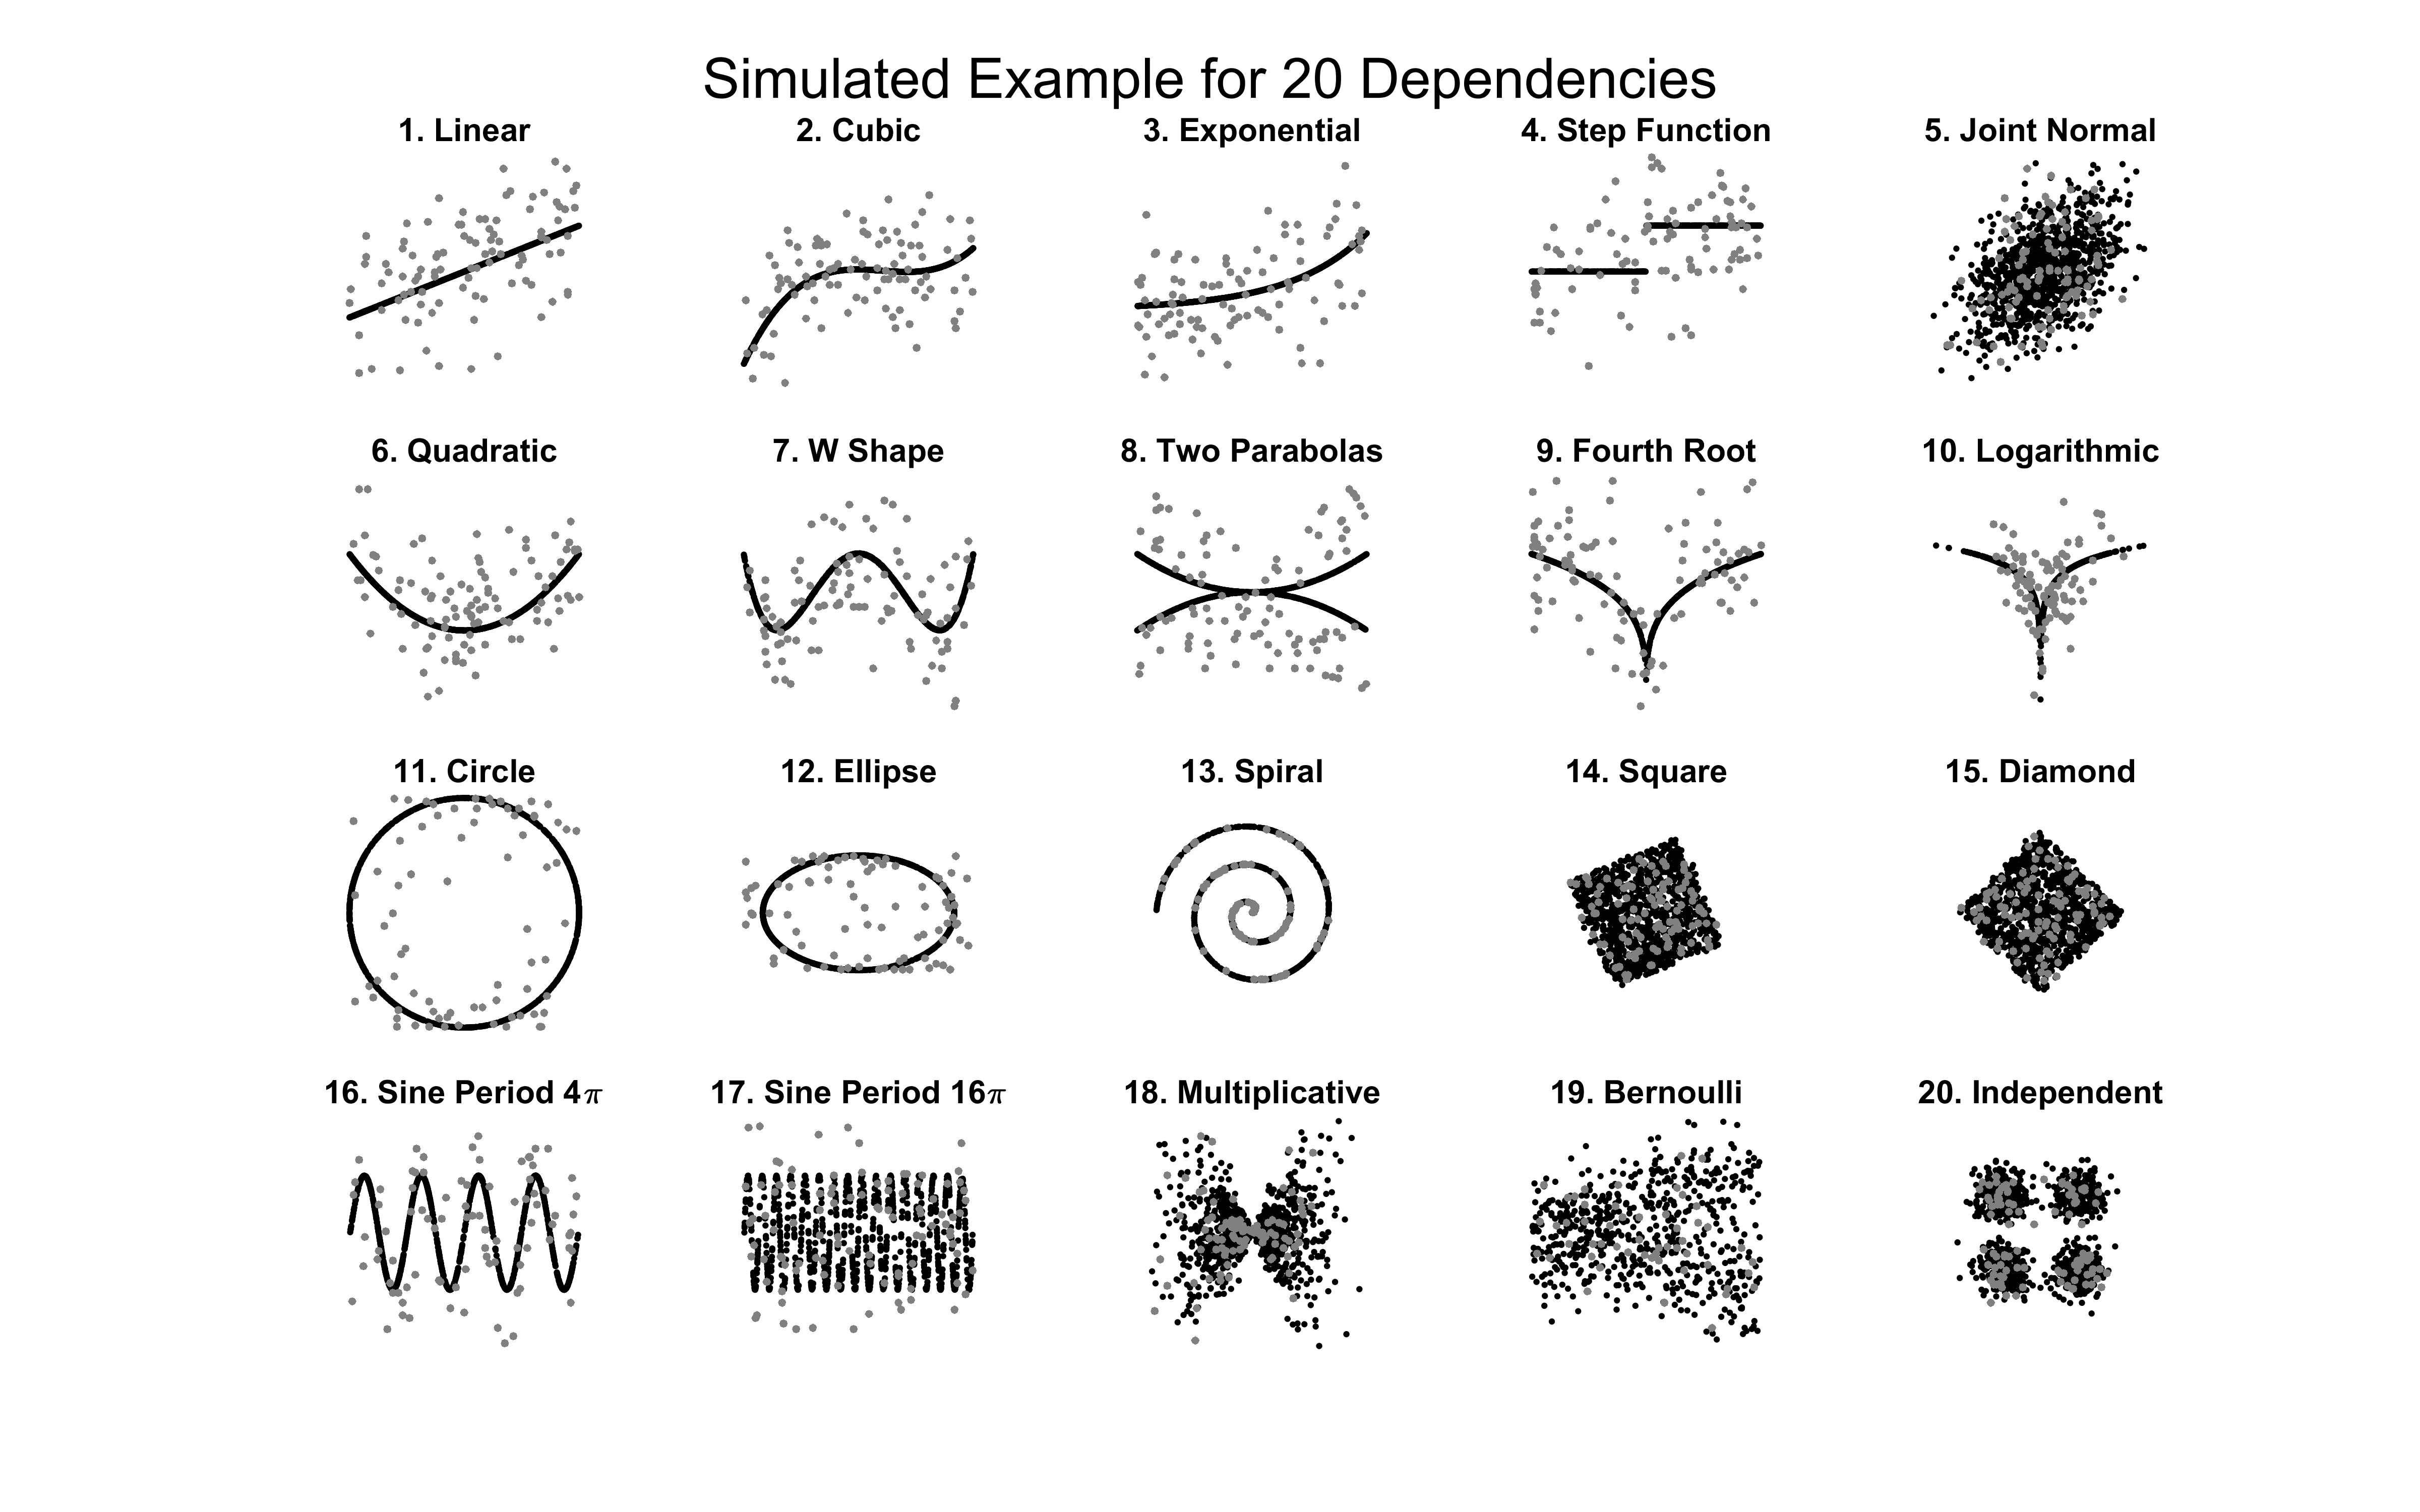
\includegraphics[trim={5cm 0 3.5cm 0},clip, width=1.0\textwidth]{../Figures/FigSimVisual}
\caption{Visualization of the $20$ dependencies for $1$-dimensional simulations. The blue points are generated with noise (c=1) at $n=100$ to show the actual sample data in testing, and the red points are generated without noise at $n=1000$ to highlight each underlying dependency.
}
\label{f:dependencies}
\end{figure}


\begin{figure}
  \centering
  \begin{tabular}{@{}p{0.4\linewidth}@{\quad}p{0.4\linewidth}@{}}
	  \centering
    \subfigimg[width=\linewidth]{A}{../Figures/Fig1DPerm} &
    \subfigimg[width=\linewidth]{B}{../Figures/FigHDPerm}
  \end{tabular}
\caption{Comparing estimated \Mgc~power to true \Mgc~power, for the $1$-dimensional and high-dimensional simulations.
(A) $1$-dimensional simulations, where $d_{x}=1$ and the sample size is chosen by the power threshold $0.8$ as in Figure~\ref{f:powermaps1}.
(B) High-dimensional simulations, where $n=100$ and the dimension is chosen by the power threshold $0.5$ as in Figure~\ref{f:powermaps}.
The estimated \Mgc~power by the approximated optimal scale is almost always better than global \Mcorr~and \Hhg, combines the better performance of the two benchmarks, is quite close to the true \Mgc~power, and does not inflate false signals.}
\label{f:simPerm}
\end{figure}


Here we also present an additional setting, which sets $d_{x}=d_{y}=1$ and $c=1$ with the sample size $n$ increasing from $5$ to $100$. The parameter before $c$ (e.g., there is a $80$ before $c$ in type 2) is a tuned noise parameter for some dependencies, so the testing powers can be compared meaningfully for each simulation, i.e., in the absence of noise, the testing powers may converge to $1$ at very small $n$ for some trivial dependencies like linear; and it is also more meaningful to consider noisy simulations in practice. The powers of all methods in this setting are provided in Figure~\ref{f:1DAll}, with the multiscale power maps shown in Figure~\ref{f:powermaps1}.

Clearly \Mgc~always improves over its global counterpart, and always has a large advantage regardless of the underlying dependency structure, the dimensionality, the sample size, or noise.

\begin{figure}[htbp]
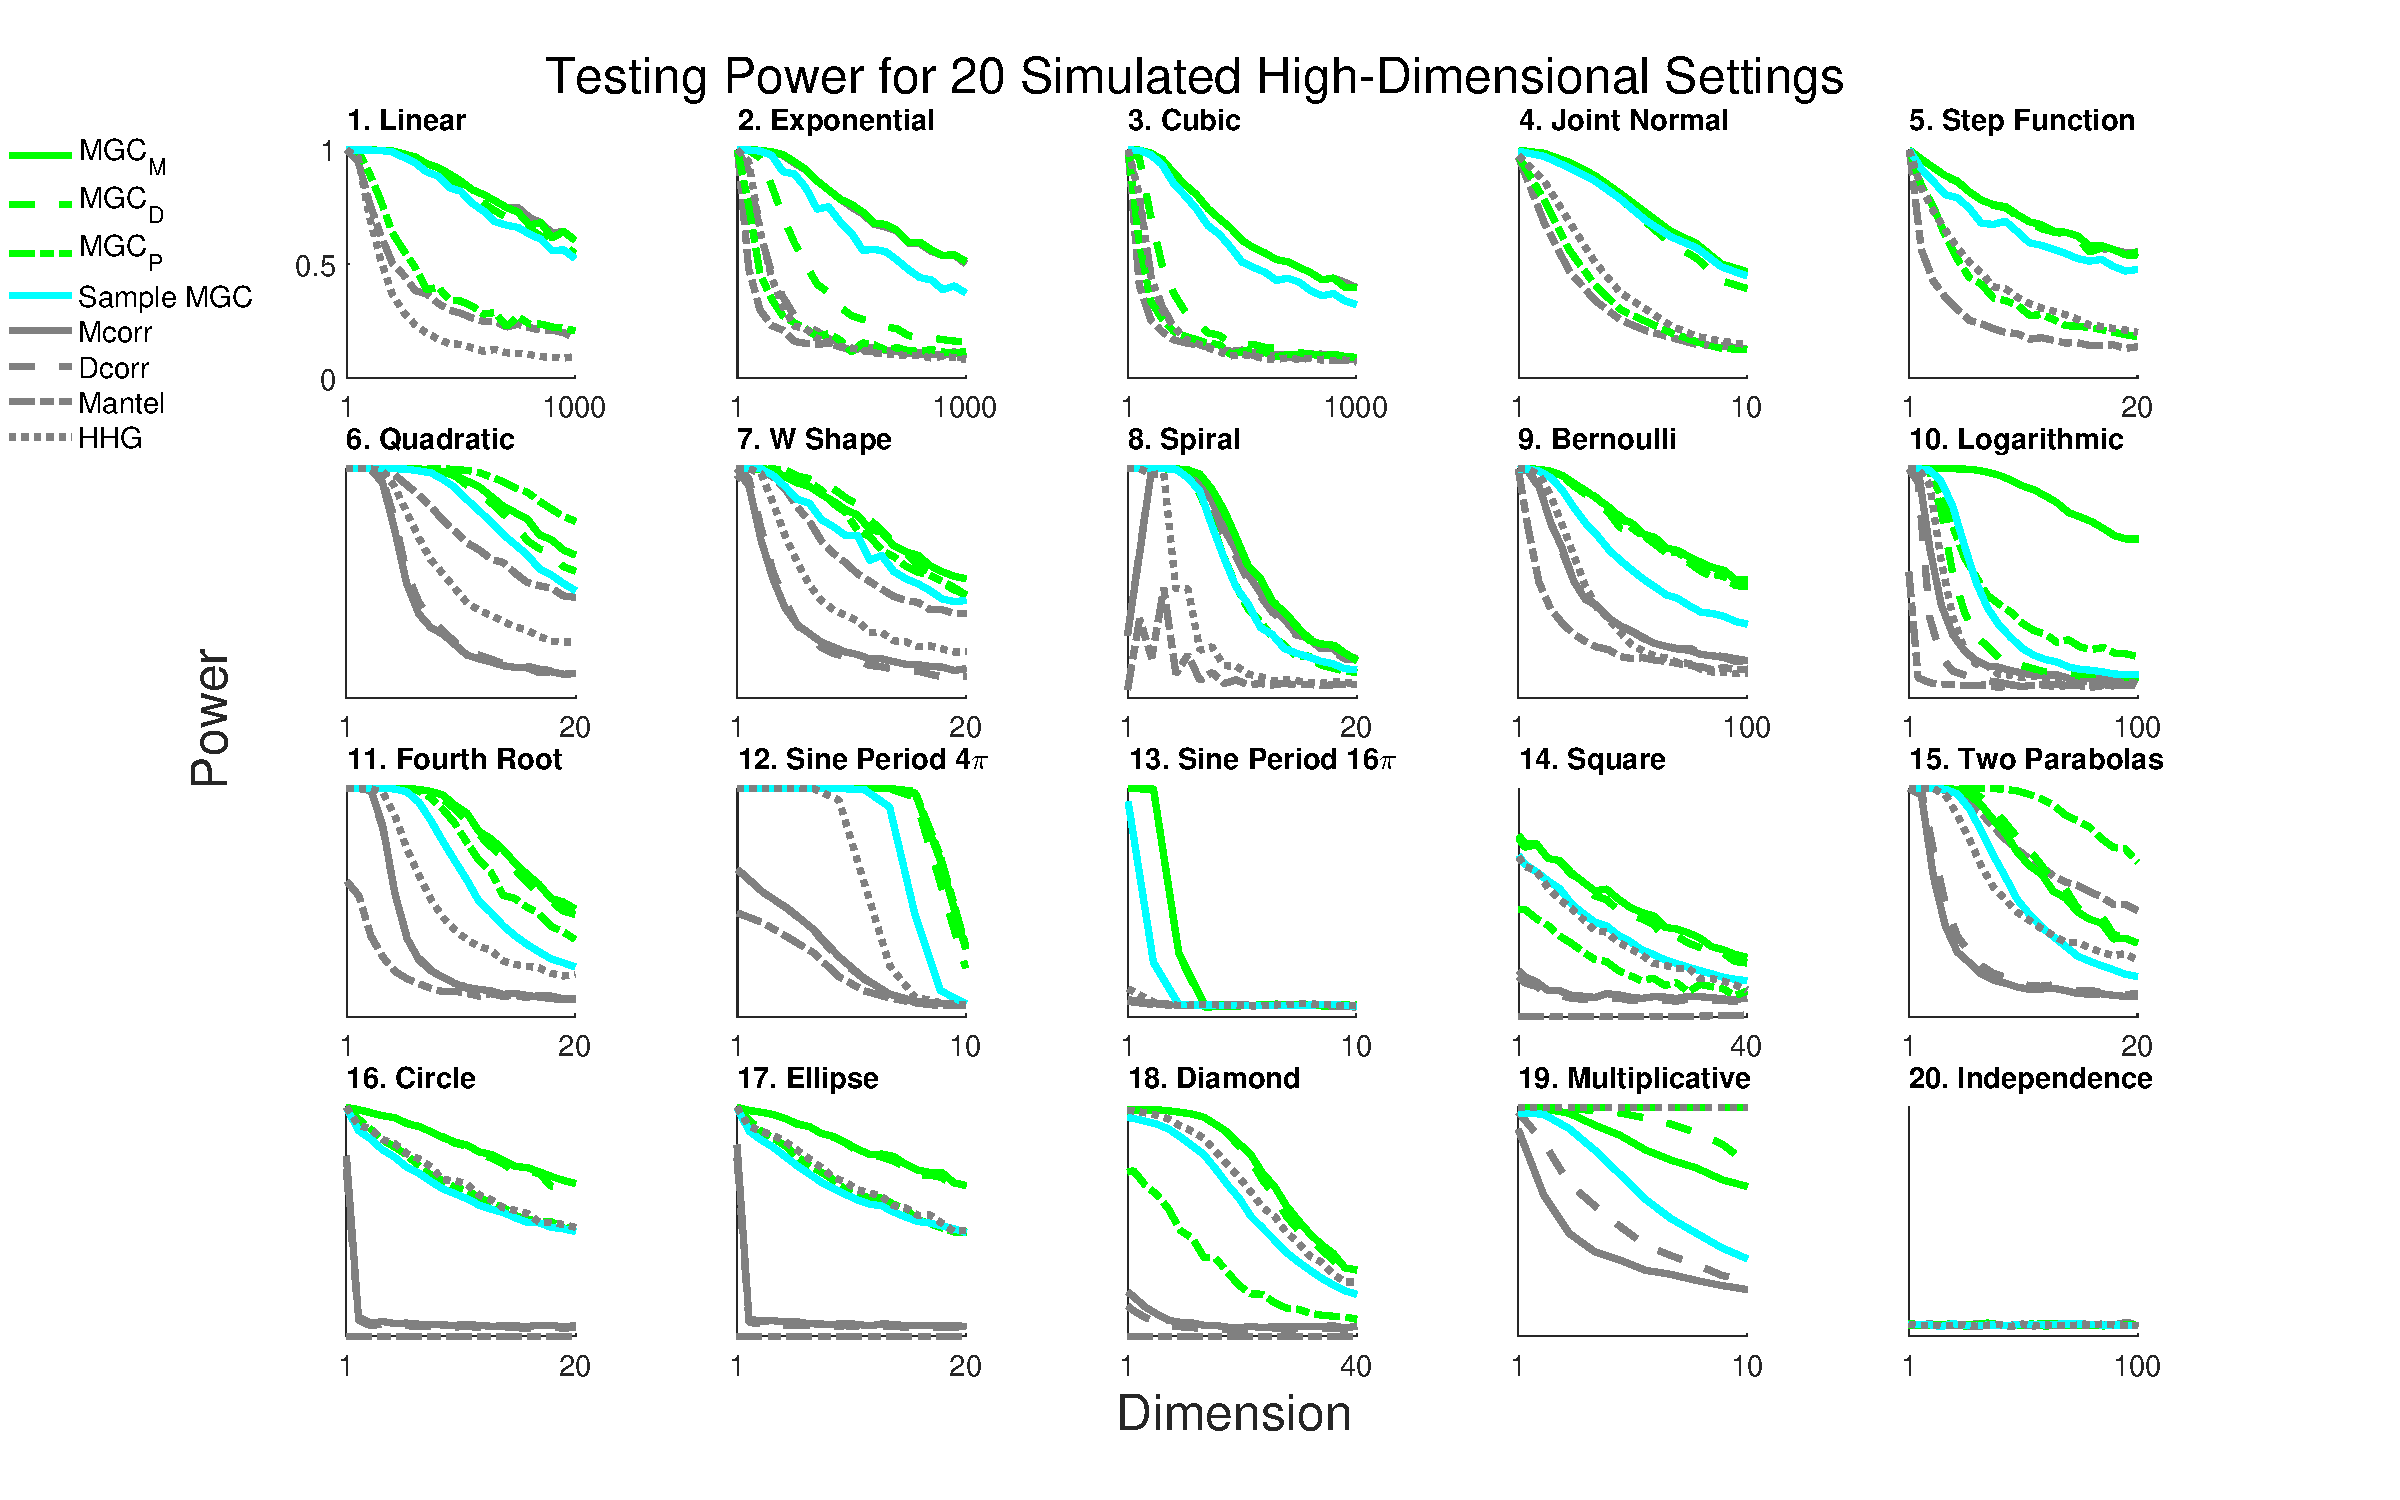
\includegraphics[width=1.0\textwidth]{../Figures/FigHDPowerAll}
\caption{
Same as Figure~\ref{f:nD} but includes all three different \Mgc~implementations.}
\label{f:nDAll}
\end{figure}

\begin{figure}[htbp]
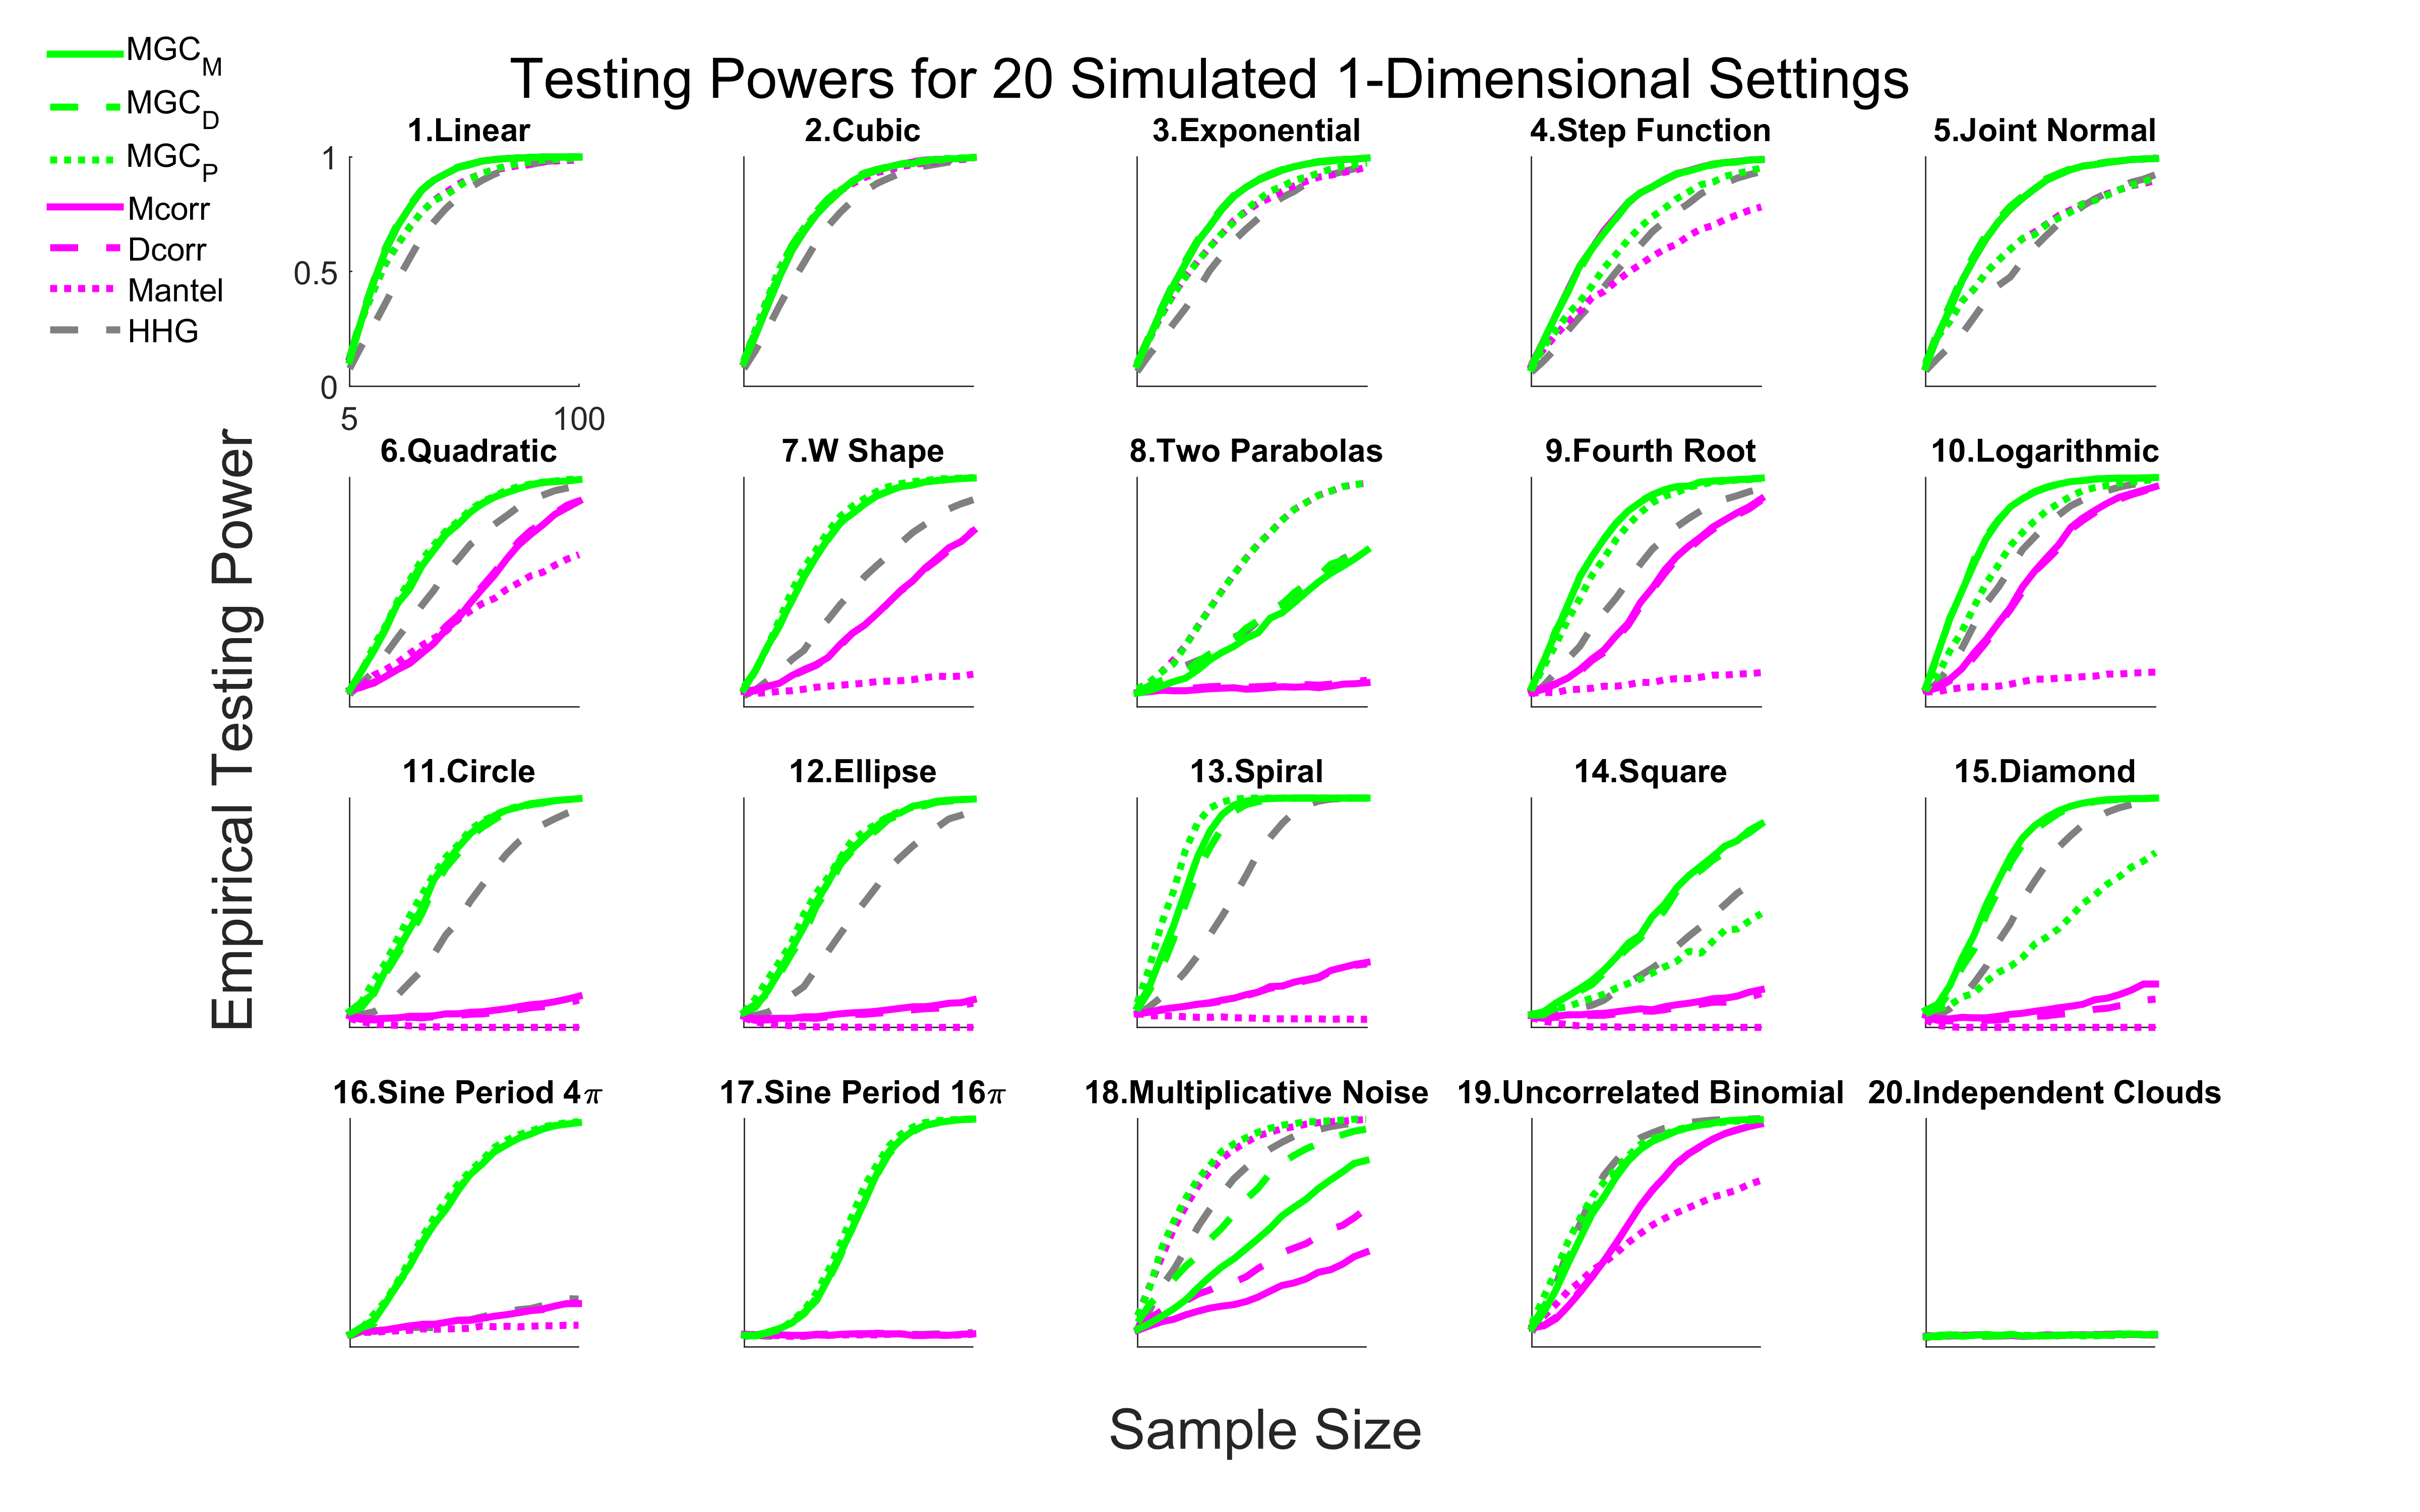
\includegraphics[width=1.0\textwidth]{../Figures/Fig1DPowerAll}
\caption{
Powers of different methods for $20$ different $1$-dimensional dependence structures, estimated by the empirical distributions of the test statistics under the null and the alternative on the basis of $10$,$000$ Monte-Carlo replicates. $2$,$000$ additional MC replicates are used for optimal scale estimation for \Mgc.
Each panel shows empirical testing power on the absicca at a significant level $\alpha=0.05$, and sample size on the ordinate.
\Mgc~empirically achieves similar or better power than the previous state of the art approaches for all sample sizes on nearly all problems.}
\label{f:1DAll}
\end{figure}

\begin{figure}[htbp]
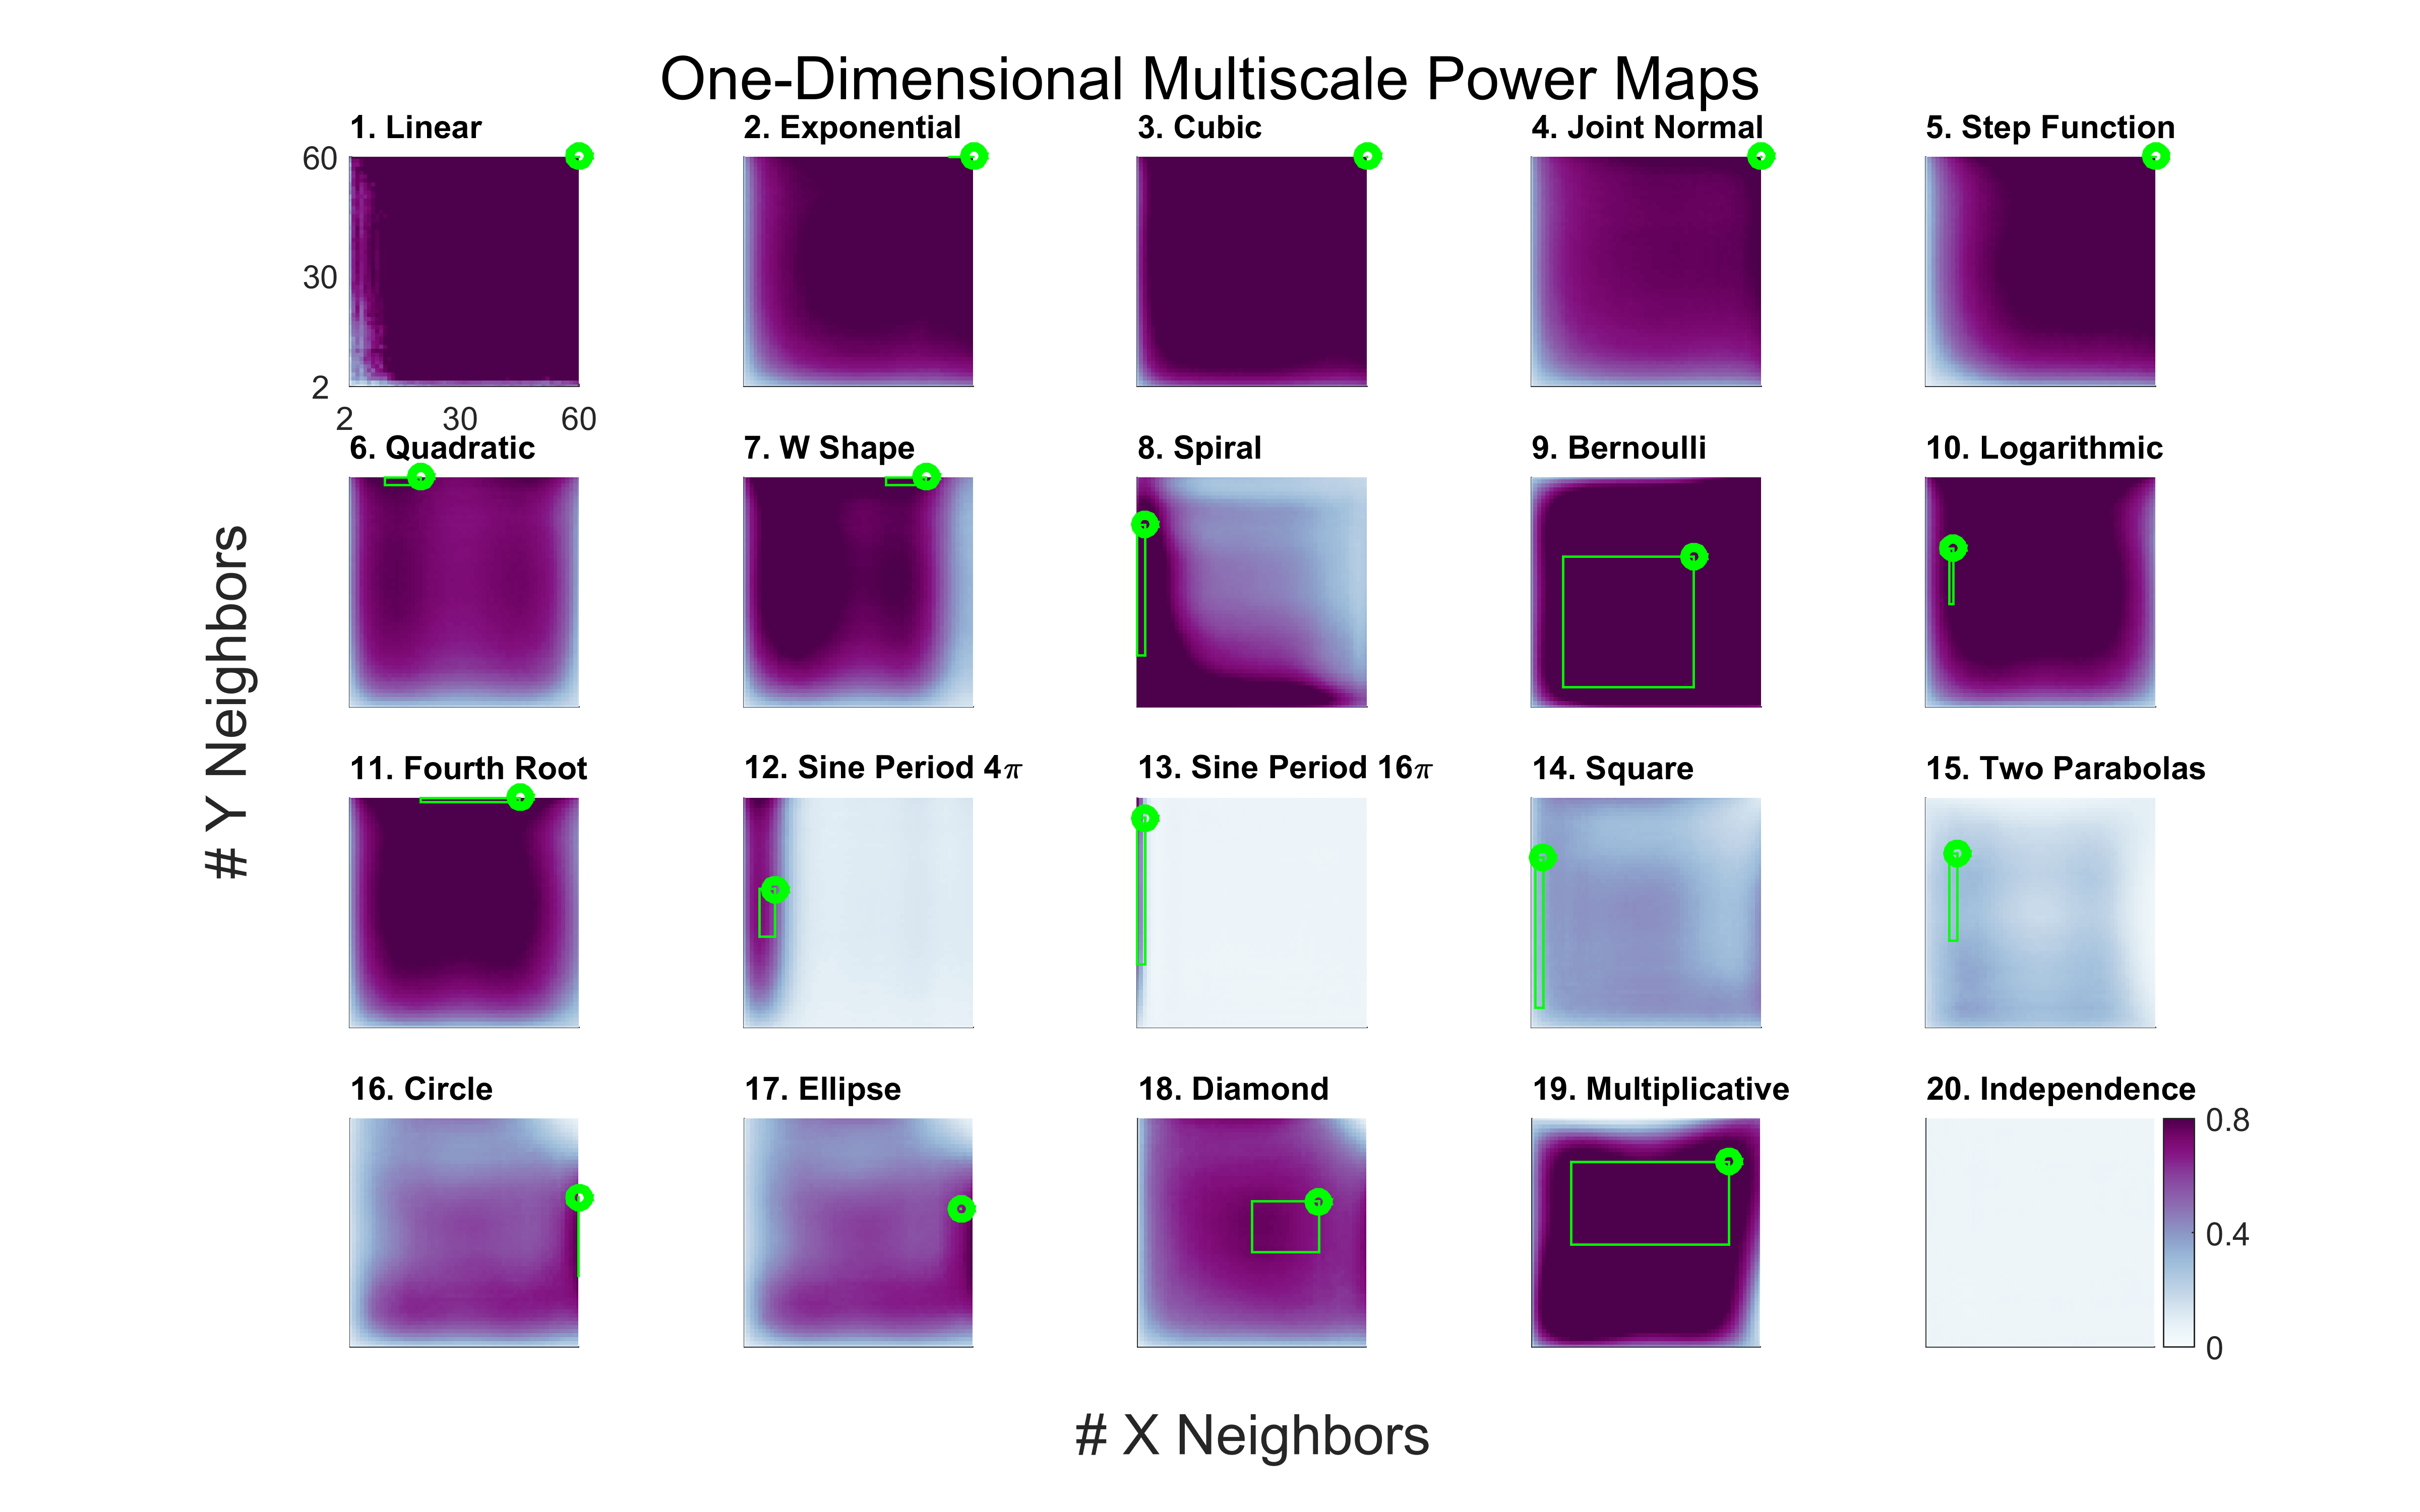
\includegraphics[width=1.0\textwidth]{../Figures/Fig1DHeat}
\caption{Influence of neighborhood size on testing power of local correlations. For each simulation, the dimension is $1$, and the sample size is determined by the first sample size $n$ for \Mgc~to have powers exceeding the threshold $0.8$.
}
\label{f:powermaps1}
\end{figure}

%\section{Performance Profiles}
%\label{appen:profiles}
%The performance profiles of each method are drawn by the following steps:

%Suppose there are $S$ methods and $T$ different problems, and the respective powers are denoted as $\beta_{\alpha}^{t}(s)$ for $s=1,\ldots,S$ and $t=1,\ldots,T$ at a fixed type 1 error $\alpha$. Then the relative performance for each method is defined as follows:
%\begin{align*}
%performance_{s}(x) &= \frac{1}{T} \sum_{t=1}^{T} \mb{I}((\beta_{\alpha}^{t}(*)-\beta_{\alpha}^{t}(s)) \leq x)
%\end{align*}
%where $x \in [0,1]$, $\mb{I}$ is the indicator function, and $\beta_{\alpha}^{t}(*) =\max \mbx_{s} \{\beta_{\alpha}^{t}(s)\}$ denotes the best testing power in the $t$th problem. Namely \mbx~stands for the difference with respect to the best power, and the relative performance of each method equals the proportion of simulations that the method is worse than the best method by no more than \mbx. For example, at $x=0.1$, \Mgc~has a relative performance of $0.75$ if and only if there are $15$ out of $20$ simulations that \Mgc~is worse than the best method by no more than $0.1$ in testing power. Note that the performance profiles at $x=0$ stands for the proportion of simulations that the method has the best power; and the curve always increases to $1$ at $x=1$.

%To better summarize the overall performance in the low-dimensional simulations, we use the performance profiles \cite{DolanMore2002}, which provides an intuitive way for directly comparing a set of algorithms on a set of problems.  Briefly, each curve (profile) shows the relative performance of a given algorithm as a function of how far from the best algorithm it performed. Therefore, higher curves and larger area under curve are better, and a more detailed description is in Appendix \ref{appen:profiles}. For each $1$-dimensional simulation, we fix the sample size by a power threshold, and draw the corresponding performance profiles of all tests in Figure~\ref{fig:pp}(A). To compare the performance profiles of each test with respect to different threshold choices, we further provide the area under curve of the performance profiles against the power threshold in Figure~\ref{fig:pp}(B).

% \begin{figure}
%   \centering
%   \begin{tabular}{@{}p{0.5\linewidth}@{\quad}p{0.5\linewidth}@{}}
%     \subfigimg[width=\linewidth]{A}{../Figures/Fig1DPP} &
%     \subfigimg[width=\linewidth]{B}{../Figures/Fig1DPPAUC} \\
%     \subfigimg[width=\linewidth]{C}{../Figures/FigHDPP} &
%     \subfigimg[width=\linewidth]{D}{../Figures/FigHDPPAUC}
%   \end{tabular}
%   \caption{Quantitative comparisons of the power of the various tests across all simulations into a single number, with $r=10$,$000$ Monte-Carlo replicates at $\alpha=0.05$ (and $2$,$000$ additional MC replicates for optimal scale estimation).
% (A) Performance profile plots comparing different methods on all 1-dimensional simulations at the first sample size $n$ of any testing power to exceed the power threshold 0.8. The legend provides the Area-Under-the-Curve (AUC) for each method; larger is better.
% (B) AUC for each method sweeping over all different power thresholds, the higher the better.
% (C) Same as (A) but for the high-dimensional simulations, at the largest dimension of any testing power that is above the power threshold $0.5$.
% (D) Same as (B) but for the high-dimensional simulations.
% It is clear that \Mgc~outperforms the previous state of the art approaches regardless of the underlying model, sample size, and dimensionality.}
% \label{fig:pp}
% \end{figure}

\section{Dependence Measures}
\label{appen:methods}

In this section, we review the \Mantel~test, distance correlation, modified distance correlation, the \Mgc~statistic, and the \Hhg~statistic in order. Note that for \Dcorr~/ \Mcorr, we implement them in a slightly different but equivalent way from the original definition.

\subsection{(Global) \Mantel~Test}
\label{appen:mantel}
Given the Euclidean distance matrices $\tilde{A}$ and $\tilde{B}$, the \Mantel~coefficient \cite{Mantel1967} is defined as
\begin{equation}
\Mantel(X,Y)=\frac{\sum_{i \neq j}^{n}(a_{ij}-\bar{a})(b_{ij}-\bar{b})}{\sqrt{\sum_{i \neq j}^{n}(a_{ij}-\bar{a})^2 \sum_{i \neq j}^{n}(b_{ij}-\bar{b})^2}},
\end{equation}
where $A=\tilde{A}$, $B=\tilde{B}$, $\bar{a}=\frac{1}{n(n-1)}\sum_{i \neq j}^{n}(a_{ij})$ and similarly for $\bar{b}$. Then the \Mantel~test is carried out by the permutation test.

Unlike distance correlation and \Hhg, the \Mantel~test is not consistent against all dependent alternatives, but it has been a very popular method in biology and ecology due to its simplicity. It is clear from Figure~\ref{f:nDAll} and ~\ref{f:1DAll} that global \Mantel~is sub-optimal and appears to be not consistent for many dependencies, yet \Mgcp~achieves comparable performances as other variants of \Mgc, which implies that \Mgcp~may be consistent against most, if not all dependent alternatives.

\subsection{(Global) Distance Correlation}
\label{appen:dcorr}
Given two distance matrices $\tilde{A}$ and $\tilde{B}$ of the sample data $X$ and $Y$, the sample distance covariance is defined by doubly centering the distance matrices:
\begin{equation}
\label{dcovEqu}
dcov(X,Y)=\frac{1}{n^2}\sum_{i,j=1}^{n}a_{ij}b_{ij},
\end{equation}
where $A=H\tilde{A}H$, $B=H\tilde{B}H$ with $H=I_{n}-\frac{J_{n}}{n}$. Then the sample distance variance is defined as
\begin{align*}
dvar(X) &=\frac{1}{n^2}\sum_{i,j=1}^{n}a_{ij}^{2},\\
dvar(Y) &=\frac{1}{n^2}\sum_{i,j=1}^{n}b_{ij}^{2},
\end{align*}
and the sample distance correlation equals
\begin{equation}
\label{dcorrEqu}
\Dcorr(X,Y)=\frac{dcov(X)}{\sqrt{dvar(X) \cdot dvar(Y)}}.
\end{equation}

It is shown in \cite{SzekelyRizzoBakirov2007} that as $n \rightarrow \infty$, $\Dcorr(X,Y) \rightarrow \Dcorr(\mb{x},\mb{y}) \geq 0$, where $\Dcorr(\mb{x},\mb{y})$ denotes the population distance correlation between the underlying random variable $\mb{x}$ and $\mb{y}$. The population distance correlation is defined by the characteristic functions, which is $0$ if and only if $\mb{x}$ and $\mb{y}$ are independent. Thus the sample distance correlation is a consistent statistic for testing independence, i.e., the testing power $\beta_{\alpha}(\Dcorr(X,Y))$
converges to $1$ as $n$ increases, at any type $1$ error level $\alpha$. Note that all of $dcov, dvar$, \Dcorr~are always non-negative; and the consistency result assumes finite second moments of $\mb{x}$ and $\mb{y}$, which holds for a family of metrics not limited to the Euclidean distance \cite{Lyons2013}. Also note that the \Dcorr~above is actually the square of distance correlation in \cite{SzekelyRizzoBakirov2007}, but for ease of presentation the square naming is dropped here.

Alternatively, calculating the distance covariance by $A=H\tilde{A}$ and $B=\tilde{B}H$ gives the same statistic as in Equation~\ref{dcovEqu}, i.e., instead of using doubly centered distance matrices, it is the same to singly center one distance matrix by row and the other distance matrix by column. Then \Dcorr~by singly centered distance matrices has the same testing power as the original \Dcorr, because distance covariance is equivalent to distance correlation in the permutation test (note that the actual \Dcorr~statistic by single centering is different from the original \Dcorr, as using single centering changes the distance variances).

In our implementation of global / local \Dcorr, we always use singly centered distance matrices rather than doubly centered distance matrices. Although they are equivalent for the testing power of global \Dcorr, our alternative implementation improves the testing power of local \Dcorr~and \Mgc. This is because the ranking information of $\tilde{A}$ and $\tilde{B}$ are better preserved in singly centered distance matrices, so that \Mgc~is more effective in excluding far-away points that exhibit insignificant dependency. This applies to \Mcorr~as well.

\subsection{(Global) Modified Distance Correlation}
\label{appen:mcorr}
In case of high-dimensional data where the dimension $d_{x}$ or $d_{y}$ increases with the sample size $n$, the sample distance correlation may no longer be appropriate. For example, even for independent Gaussian distributions, $\Dcorr(X,Y) \rightarrow 1$ as $d_{x}, d_{y} \rightarrow \infty$, which may severally impair the testing power of sample \Dcorr~in high-dimensional simulations.

The modified distance correlation is proposed in \cite{SzekelyRizzo2013a} to tackle the bias of sample \Dcorr. Denote the Euclidean distance matrices as $\tilde{A}$ and $\tilde{B}$, the doubly centered distance matrices as $\hat{A}$ and $\hat{B}$, the modified distance covariance is defined as
\begin{equation}
\label{mcovEqu}
mcov(X,Y)=\frac{n}{(n-1)^2(n-3)}(\sum_{i \neq j}^{n}a_{ij}b_{ij}-\frac{2}{n-2}\sum_{j=1}^{n}a_{jj}b_{jj}),
\end{equation}
where $A$ modifies the entries of $\hat{A}$ by
\[a_{ij} = \left\{
  \begin{array}{lr}
    \hat{a}_{ij}-\frac{\tilde{a}_{ij}}{n}, & \mbox{ if } i \neq j, \\
    \frac{n\sum_{i}\tilde{a}_{ij}-\sum_{i,j}\tilde{a}_{ij}}{n^2}, &\mbox{ if } i = j,
  \end{array}
\right.
\]
and so is $B$. Then $mvar(X)$ and $mvar(Y)$ can be similarly defined.

If $mvar(X) \cdot mvar(Y) \leq 0$, the modified distance correlation is set to $0$ (negativity can only occur when $n\leq 2$, equality can only happen in some special cases); otherwise it is defined as
\begin{equation}
\label{mcorrEqu}
\Mcorr(X,Y)=\frac{mcov(X,Y)}{\sqrt{mvar(X) \cdot mvar(Y)}}.
\end{equation}

It is shown in \cite{SzekelyRizzo2013a} that $\Mcorr(X,Y)$ is an unbiased estimator of the population distance correlation $\Dcorr(\mb{x},\mb{y})$ for all $d_{x}, d_{y}, n$; and \Mcorr~is approximately normal even if $d_{x},d_{y} \rightarrow \infty$. Thus it is a consistent statistic for testing independence, but may work better than \Dcorr~under high-dimension dependencies.

Similar to the alternative implementation of \Dcorr, we can also use singly centered distance matrices for $\hat{A}$ and $\hat{B}$ in defining \Mcorr, which does not alter the theoretical advantages of original \Mcorr. We further set $A_{ii}=B_{ii}=0$ for all $i$, which simplifies the expression of \Mcorr~and is asymptotically equivalent for the testing purpose.

%Also note that when there exists repeating points, it is necessary to set $a_{ij}=a_{jj}$ for repeating points during global/local mcorr computation, or exclude repeating observation before-hand, otherwise the diagonal adjustment of mcorr may lose its effect for adjusting high-dimensional bias.

\subsection{Multiscale Graph Correlations (\Mgc)}
\label{appen:mgc}
For any generalized correlation coefficient, its local correlations can be directly implemented as in Equation~\ref{localCoef}, by plugging in the respective $a_{ij}$ and $b_{ij}$ from Equation~\ref{generalCoef} and sorting the distance matrices column-wise as in Equation~\ref{localCoef2}.

In particular, \Mantel~sets $a_{ij}$ and $b_{ij}$ as the respective entry of $\tilde{A}$ and $\tilde{B}$ (the Euclidean distances). \Dcorr~lets $a_{ij}$ and $b_{ij}$ be the respective matrix entry of $A$ and $B$ (the doubly centered distance matrices), then the sample means $\bar{a}, \bar{b}$ are automatically $0$. \Mcorr~slightly modifies $a_{ij}$ and $b_{ij}$ of \Dcorr~to adjust their high-dimensional bias. As discussed already, our version of \Mgcm~is based on single centering throughout: we take $a_{ij}=b_{ij}=0$ when $i=j$, otherwise set $a_{ij}$ as the matrix entry of $H\tilde{A}-\tilde{A}/n$, and set $b_{ij}$ as the entry of $\tilde{B}H-\tilde{B}/n$. Then the local version of \Mcorr~follows by Equation~\ref{localCoef}.

Generally, there are a total of $\max(R(a_{ij})) \times \max(R(b_{ij}))$ local correlations, which equals $n^2$ when there exists no repeating data. Note that we use minimal ranks in sorting when ties occur, which indexes all local correlations more conveniently than breaking ties randomly or using average / max ranks.

Among all possible local correlations, MGC picks the optimal local correlation that yields the best testing power. The optimal scale clearly exists, but is distribution dependent and is almost always non-unique. Among all local correlations, it suffices to exclude $\G^{1l}$ and $\G^{k1}$ for testing and optimal scale estimation: since $\G^{1l}=\G^{k1}=\G^{11}$, they do not include any neighbor other than each observation itself, merely count the diagonal terms in the distance matrices, and are not meaningful for the testing purpose.

%Another technical detail worth mentioning: in our definition of $\bar{a}^{k}, \sigma_a^{k}, \bar{b}^{l}, \sigma_b^{l}$, they are computed from all entries of $a_{ij}^k$ and $b_{ij}^l$, e.g., $\bar{a}^{k}$ equals $\dfrac{1}{n^2} \sum_{i,j=1}^{n} a_{ij}^k$. Alternatively, one may exclude the zero entries in computing the means and standard deviations of the truncated comparisons, i.e., $\bar{a}^{k}=\dfrac{1}{nk} \sum_{i,j=1}^{n} a_{ij}^k$ for \Dcorr, etc., then properly adjust the scalar factor $n^2$ in $z_{kl}$. But for ease of presentation, we presented the more intuitive definition in the main paper, which is empirically equivalent to the alternative definition for the testing purpose.

\subsection{Heller, Heller \& Gorfine (\Hhg)}
\label{appen:hhg}
The \Hhg~statistic applies Pearson's chi-square test to ranks of distances within each column, and is shown to be better than many global tests including \Dcorr~under common nonlinear dependencies in \cite{GorfineHellerHeller2012, HellerGorfine2013}. Like \Dcorr~and \Mcorr, \Hhg~is distance-based and consistent, but not in the form of the generalized correlation coefficient; and like our \Mgc, it makes use of the rank information, but in a distinct manner.

Given the Euclidean distance matrices $\tilde{A}=[\tilde{a}_{ij}]$ and $\tilde{B}=[\tilde{b}_{ij}]$, we denote
\begin{align*}
H_{11}(i,j) &= \sum_{q=1,q\neq i,j}^{n}I(\tilde{a}_{ik} \leq \tilde{a}_{ij})I(\tilde{b}_{ik} \leq \tilde{b}_{ij}) \\
H_{12}(i,j) &= \sum_{q=1,q\neq i,j}^{n}I(\tilde{a}_{ik} \leq \tilde{a}_{ij})I(\tilde{b}_{ik} > \tilde{b}_{ij}) \\
H_{21}(i,j) &= \sum_{q=1,q\neq i,j}^{n}I(\tilde{a}_{ik} > \tilde{a}_{ij})I(\tilde{b}_{ik} \leq \tilde{b}_{ij}) \\
H_{22}(i,j) &= \sum_{q=1,q\neq i,j}^{n}I(\tilde{a}_{ik} > \tilde{a}_{ij})I(\tilde{b}_{ik} > \tilde{b}_{ij}),
\end{align*}
and the \Hhg~statistic is defined as
\begin{align*}
\Hhg(X,Y) &= \sum_{i=1,j\neq i}^{n} \frac{(n-2)(H_{12}(i,j)H_{21}(i,j)-H_{11}(i,j)H_{22}(i,j))^2}{H_{1 \cdot}(i,j)H_{2 \cdot}(i,j)-H_{\cdot 1}(i,j)H_{\cdot 2}(i,j)},
\end{align*}
where $H_{1 \cdot}=H_{11}+H_{12}$, $H_{2 \cdot}=H_{21}+H_{22}$, $H_{\cdot 1}=H_{11}+H_{21}$, and $H_{\cdot 2}=H_{12}+H_{22}$. It is clear that \Hhg~is structurally different from \Dcorr~/ \Mcorr~/ \Mantel, cannot be conveniently expressed by Equation~\ref{generalCoef}, and there is no direct extension of local correlation to \Hhg.

The permutation test using the \Hhg~statistic is consistent against all dependent alternatives. In our numerical simulations, \Hhg~falls a bit short when testing against high-dimensional and noisy linear dependencies, but is often more advantageous than global correlations under nonlinear dependencies, which makes it a strong competitor in general.

\section{\Mgc~Algorithms and Testing Procedures}
\label{appen:tests}
In this section we elaborate on the algorithms for computing local correlation and \Mgc, as well as their testing procedures in simulations and real data experiment.

Five algorithms are presented in section~\ref{appen:algorithms}: given the choice of a global correlation coefficient, algorithm~\ref{alg:1scale} computes one local correlation coefficient at a given $(k,l)$; then algorithm~\ref{alg:all_scales} shows how to compute all local correlations simultaneously; algorithm~\ref{alg:pval} computes the p-values of all local correlation by the random permutation test; algorithm~\ref{alg:best_scale} approximates the optimal scale for \Mgc~based on the p-values of all local correlations, and outputs the approximated p-value of \Mgc; algorithm~\ref{alg:power} estimates the testing powers of all local statistics based on a given joint distribution or multiple pairs of data, which can be used to more accurately estimate the optimal scale for \Mgc~when the underlying model is known or training data are given. More detailed discussions regarding the optimal scale approximation is offered in section~\ref{appen:diss}.

\subsection{Algorithms}
\label{appen:algorithms}
All algorithms are implemented in Matlab and R with the pseudo-code shown below. For ease of presentation, we assume there are no repeating data and take \Dcorr~as the global correlation in the pseudo-code.

Algorithm~\ref{alg:1scale} shows a straightforward computation of one local correlation coefficient, which requires $O(n^2)$ once the rank information is provided. This is suitable for \Mgc~computation when the optimal local scale is known or already estimated. But using algorithm~\ref{alg:1scale} to compute all local correlations would require iterating through all possible neighborhoods $(k,l)$, which takes $O(n^4)$ and would make the optimal scale estimation computationally inefficient.

To facilitate the optimal scale estimation, algorithm~\ref{alg:all_scales} provides a fast method to compute all local correlations in $O(n^2)$. An important observation is that each product $a_{ij}b_{ij}$ is included in $\G^{kl}$ if and only if $(k,l)$ satisfies $k\leq R(a_{ij})$ and $l\leq R(b_{ij})$, so it suffices to iterate through $a_{ij}b_{ij}$ for $i,j=1,\ldots,n$, and add the product simultaneously to all $\G^{kl}$
whose scales are no more than $(R(a_{ij}),R(b_{ij}))$. However, accessing and adding multiple $\G^{kl}$ at the same time is not computationally efficient; instead, for each product, we only add it to $\G^{kl}$ at $(k,l)=(R(a_{ij}),R(b_{ij}))$ (so only one local scale is accessed for each operation), iterate through all products for $i,j=1,\ldots,n$, then add up adjacent $\G^{kl}$ for $k,l=1,\ldots,n$. Thus all local correlations can be computed in $O(n^2)$, which has the same running time complexity as the global distance correlation. There are two additional overheads: sorting the distance matrices column-wise takes $O(n^2 \log n)$, and properly centering the distance matrices takes $O(n^2)$.

Algorithm~\ref{alg:pval} computes the p-values of all local correlation by the permutation test with $r$ random permutations, which takes $O(rn^2 \log n)$.

Algorithm~\ref{alg:best_scale} approximates the optimal scale $(k^{*},l^{*})$ from the p-values of all local correlations, and outputs the approximated \Mgc~p-value. This is necessary for testing on one pair of data with unknown model, while algorithm~\ref{alg:power} is more appropriate for known model. Conceptually, the algorithm first searches for a set of ``valid'' adjacent rows $\K=\{k_{1},k_{1}+1,\ldots,k_{2}-1,k_{2}\}$ such that the median p-value of $\{p_{kl},k \in \K, l=2,\ldots,n\}$
is no larger than $\alpha /(n-1) * |\K|$, otherwise we take $\K=\{n\}$; and similarly determine the set of valid columns $\LL$. Once $\K$ and $\LL$ are determined, the optimal scale $(k^{*},l^{*})$ is found by the scale that minimizes the p-value within $\{p_{kl},k \in \K, l \in \LL\}$. Clearly if the majority p-values of all local correlations are less than $\alpha$, then $\K=\LL=\{1,\ldots,n\}$, and the optimal scale equals the scale that minimizes the p-values among all local correlations; if there is no valid rows and columns, then \Mgc~takes the largest scale and equals the global correlation. Note that the actual algorithm is a simpler version of the above description: instead of considering all possible sets of rows and check the validity, we limit the check to the most likely set of rows, by first looking for the row scale of the smallest p-value, then including all adjacent rows whose minimal p-value on the row is no larger than $\alpha$; similarly for the set of columns.

Algorithm~\ref{alg:power} computes the testing powers of all local correlations by repeated simulating samples generated from the joint distribution $f_{xy}$. Sample data under the null and the alternative are repeatedly generated for $r$ Monte-Carlo replicates, and algorithm~\ref{alg:all_scales} is applied to compute the sample local correlations under the null and the alternative. Then the testing power at each local correlation can be estimated, and the \Mgc~optimal scale can be found by maximizing the powers. This algorithm is also applicable if there exists multiple pairs of data with unknown model but similar dependency structure, then the alternative statistic can be computed from each data pair while the null statistic can be computed from each data pair under permutation. The running time is $O(rn^2 \log n)$.

\begin{algorithm}
\caption{Local Correlation Computation for One Scale}
\label{alg:1scale}
\begin{algorithmic}[1]
\Statex Input: A pair of distance matrices $(\tilde{A},\tilde{B}) \in \Real^{n \times n} \times \Real^{n \times n}$, and the given local scale $(k,l) \in \Real \times \Real$.
\Statex Output: The local correlation coefficient $\G^{kl} \in [-1,1]$ at the given $(k,l)$.
\Function{LocalCorr}{$\tilde{A}$,$\tilde{B}$,$k$,$l$}
\State initialize $\G^{kl}$, $V^{A}_{k}$, $V^{B}_{l}$, $E^{A}_{k}$, $E^{B}_{l}$ as $0$.
\Linefor{$Z:=A,B$}{$R^{Z}=\textsc{Sort}(\tilde{Z})$} \Comment{column-wise sorting and assume no ties}
\Linefor{$Z:=A,B$}{$Z=\textsc{Center}(\tilde{Z})$} \Comment{proper centering of the distance matrices}
\For{$i,j=1,\ldots,n$}
\State $\G^{kl}=\G^{kl}+A_{ij}B_{ij}\mb{I}(R^{A}_{ij} \leq k)\mb{I}(R^{B}_{ij} \leq l)$ \Comment{store local distance covariance}
\State $V^{A}_{k}=V^{A}_{k}+A_{ij}^2\mb{I}(R^{A}_{ij} \leq k)$ \Comment{store local distance variance for $X$}
\State $V^{B}_{l}=V^{B}_{l}+B_{ij}^2\mb{I}(R^{B}_{ij} \leq l)$ \Comment{store local distance variance for $Y$}
\State $E^{A}_{k}=E^{A}_{k}+A_{ij}\mb{I}(R^{A}_{ij} \leq k)$ \Comment{store the sample means}
\State $E^{B}_{l}=E^{B}_{l}+B_{ij}\mb{I}(R^{B}_{ij} \leq l)$
\EndFor

\State $\G^{kl}=\left(\G^{kl}-E^{A}_{k}E^{B}_{l}/n^2\right)/\sqrt{\left(V^{A}_{k}-{E^{A}_{k}}^2/n^2\right) \left(V^{B}_{l}-{E^{B}_{l}}^2/n^2\right)}$ \Comment{normalize the local covariances}

\EndFunction
\end{algorithmic}
\end{algorithm}

\begin{algorithm}
\caption{$O(n^2 \log n)$ Algorithm for Computing All Local Correlations}
\label{alg:all_scales}
\begin{algorithmic}[1]
\Statex Input: A pair of distance matrices $(\tilde{A},\tilde{B}) \in \Real^{n \times n} \times \Real^{n \times n}$.
\Statex Output: All local correlation coefficients $\G^{kl} \in [-1,1]^{n \times n}$ for $k,l=1,\ldots,n$.
\Function{LocalCorr}{$\tilde{A}$,$\tilde{B}$}
\State initialize $\G$ as a zero matrix of size $n \times n$; $V^{A}$, $V^{B}$, $E^{A}$, $E^{B}$ as zero vectors of size $n$.
\Linefor{$Z:=A,B$}{$R^{Z}=\textsc{Sort}(\tilde{Z})$}
\Linefor{$Z:=A,B$}{$Z=\textsc{Center}(\tilde{Z})$}
\For{$i,j=1,\ldots,n$}
\State $k=R^{A}_{ij}$
\State $l=R^{B}_{ij}$
\State $\G^{kl}=\G^{kl}+A_{ij}B_{ij}$
\State $V^{A}_{k}=V^{A}_{k}+A_{ij}^2$
\State $V^{B}_{l}=V^{B}_{l}+B_{ij}^2$
\State $E^{A}_{k}=E^{A}_{k}+A_{ij}$
\State $E^{B}_{l}=E^{B}_{l}+B_{ij}$
\EndFor
\Statex \Comment{the next two for loops with respect to the scales guarantee the computation of all local covariance / variance in $O(n^2)$}
\For{$k=1,\ldots,n-1$}
\State $\G^{1, k+1}=\G^{1, k}+\G^{1, k+1}$
\State $\G^{k+1,1}=\G^{k+1,1}+\G^{k+1,1}$
\Linefor{$Z:=A,B$}{$V^{Z}_{k+1}=V^{Z}_{k}+V^{Z}_{k+1}$}
\Linefor{$Z:=A,B$}{$E^{Z}_{k+1}=E^{Z}_{k}+E^{Z}_{k+1}$}
\EndFor

\For{$k,l=1,\ldots,n-1$}
\State $\G^{k+1,l+1}=\G^{k+1,l}+\G^{k,l+1}+\G^{k+1,l+1}-\G^{k,l}$
\EndFor

\For{$k,l=1,\ldots,n$} \Comment{normalize all local covariances}
\State $\G^{kl}=\left(\G^{kl}-E^{A}_{k}E^{B}_{l}/n^2\right)/\sqrt{\left(V^{A}_{k}-{E^{A}_{k}}^2/n^2\right) \left(V^{B}_{l}-{E^{B}_{l}}^2/n^2\right)}$
\EndFor
\EndFunction
\end{algorithmic}
\end{algorithm}

\begin{algorithm}
\caption{P-value Computation for All Local Correlations}
\label{alg:pval}
\begin{algorithmic}[1]
\Statex Input: A pair of distance matrices $(\tilde{A},\tilde{B}) \in \Real^{n \times n} \times \Real^{n \times n}$, the number of permutations $r$.
\Statex Output: The p-value matrix $P \in [0,1]^{n \times n}$ for all local distance correlations.
\Function{PermutationTest}{$\tilde{A}$,$\tilde{B}$,$r$}
\State $\G^{kl}=\textsc{LocalCorr}(\tilde{A},\tilde{B})$ \Comment{calculate the observed local correlations}
\For{$j=1,\ldots,r$}
\State $\pi=\textsc{RandPerm}(n)$ \Comment{generate a random permutation of size $n$}
\State $\G^{kl}_{0}[j]=\textsc{LocalCorr}(\tilde{A},\tilde{B}(\pi,\pi))$ \Comment{calculate the permuted test statistics}
\EndFor

\For{$k,l=1,\ldots,n$}
\State $P_{kl}=\sum_{j=1}^{r}(\G^{kl}<\G^{kl}_{0}[j])/r$ \Comment{get the p-value at each local scale}
\EndFor
\EndFunction
\end{algorithmic}
\end{algorithm}

\begin{algorithm}
\caption{Optimal Local Scale Approximation by P-values}
\label{alg:best_scale}
\begin{algorithmic}[1]
\Statex Input: The p-value matrix $P \in \Real^{n \times n}$ of all local distance correlations, the type $1$ error level $\alpha$.
\Statex Output: The approximated \Mgc~optimal scale $(k^{*},l^{*})$, and the approximated \Mgc~p-value $p$.
\Function{MGCScaleVerify}{$P$, $\alpha$}
\State $\K=\textsc{VerifyRow}(P,\alpha)$ \Comment{search for a set of valid row indices}
\State $\LL=\textsc{VerifyRow}(P\T,\alpha)$ \Comment{search for a set of valid column indices}
\State $[k^{*},l^{*}]=\arg\min_{\left\{k \in \K, l \in \LL\right\}} P_{kl}$ \Comment{find the optimal scale within the valid range}
\State $p=P_{k^{*}l^{*}}$
\EndFunction
\end{algorithmic}

\begin{algorithmic}[1]
\Statex
\Statex Input: Same as \textsc{MGCScaleVerify}.
\Statex Output: The indices of valid rows.
\Function{VerifyRow}{$P$, $\alpha$}
\State initialize $\K$ as an empty set
\State $[k^{*},l^{*}]=\arg\min_{k, l} \{P_{kl},k,l=2,\ldots,n\}$
\For{$k=k^{*},\ldots,2$} \Comment{check all row scales no larger than $k^{*}$}
\If{$\min\{P_{kl},l=2,\ldots,n\}>\alpha$}
\State break
\EndIf
\State $\K=[k,\K]$
\EndFor
\For{$k=k^{*}+1,\ldots,m$} \Comment{check all row scales larger than $k^{*}$}
\If{$\min\{P_{kl},l=2,\ldots,n\}>\alpha$}
\State break
\EndIf
\State $\K=\{\K,k\}$
\EndFor
\If{$\textsc{Median}(P_{kl},k \in \K, l=2,\ldots,n) > \alpha * \frac{|\K|}{n-1}$}
\State $\K=\{n\}$ \Comment{take the largest scale if the median p-value is not sufficiently small}
\EndIf
\EndFunction
\end{algorithmic}
\end{algorithm}

\begin{algorithm}
\caption{Testing Powers Computation for All Local Correlations}
\label{alg:power}
\begin{algorithmic}[1]
\Require A joint distribution $f_{xy}$, the sample size $n$, the number of MC replicates $r$, and the type $1$ error level $\alpha$.
\Ensure The power matrix $\beta_{\alpha} \in [0,1]^{n \times n}$ for all local correlations, and the \Mgc~optimal scale $(k^{*},l^{*}) \in \Real \times \Real$.
\Function{TestingPowers}{$f_{xy}$,$n$, $r$,$\alpha$}
\For{$j=1,\ldots,r$}
\Linefor{$i:=[n]$}{$(X^{1}_{i},Y^{1}_{i}) \stackrel{iid}{\sim} f_{xy}$} \Comment{generate dependent samples}
\Linefor{$i:=[n]$}{$X^{0}_{i} \stackrel{iid}{\sim} f_{x}$} \Comment{generate independent samples}
\Linefor{$i:=[n]$}{$Y^{0}_{i} \stackrel{iid}{\sim} f_{y}$}
\Linefor{$Z:=A,B$}{$\tilde{Z}_{1}=\textsc{Dist}(Z_{1})$} \Comment{the distance matrices under the alternative}
\Linefor{$Z:=A,B$}{$\tilde{Z}_{0}=\textsc{Dist}(Z_{0})$} \Comment{the distance matrices under the null}
\State $\G^{kl}_{1}[j]=\textsc{LocalCorr}(\tilde{A}_{1},\tilde{B}_{1})$ \Comment{calculate all local correlations under the alternative}
\State $\G^{kl}_{0}[j]=\textsc{LocalCorr}(\tilde{A}_{0},\tilde{B}_{0})$ \Comment{calculate all local correlations under the null}
\EndFor

\For{$k,l=1,\ldots,n$}
\State $c_{\alpha}=\textsc{Cdf}_{1-\alpha}(\G^{0}_{kl}[j],j \in [r])$ \Comment{get the critical value by the empirical cumulative distribution under the null at each scale}
\State $\beta_{\alpha}^{kl}=\sum_{j=1}^{r}(\G^{1}_{kl}[j]>c_{\alpha}) / r$ \Comment{estimate the power}
\EndFor
\State $(k^{*},l^{*})=\arg\max(\beta_{\alpha}^{kl})$ \Comment{find the optimal local scale}
\EndFunction
\end{algorithmic}
\end{algorithm}

\subsection{Discussions of Optimal Scale Estimation}
\label{appen:diss}
To evaluate \Mgc~in simulations or real data, the optimal scale for \Mgc~always needs to be estimated first. Algorithm~\ref{alg:power} computes the testing powers of all local correlations for known model, so the optimal scale $(k^{*},l^{*})$ can be directly estimated by maximizing the testing powers (if there are more than one optimal scales, one may pick the scale that maximizes the mean difference of the test statistic under the null and the alternative). Once the optimal scale is determined, the testing power of \Mgc~under the given model can be quickly determined by algorithm~\ref{alg:power}, and its p-value for testing on a particular pair of data can be determined by algorithm~\ref{alg:pval}.

If there is only one pair of data $(X,Y)$ with unknown distributions, we have to approximate the optimal scale by algorithm~\ref{alg:best_scale}. It makes use of Bonferroni correction to separately verify the set of rows and columns, which guarantees the false positive rate to be no higher than $\alpha$; otherwise the scale is set to the largest, which guarantees the approximated \Mgc~is at least as powerful as the global correlation. Still, algorithm~\ref{alg:best_scale} is a heuristic approach to approximate the optimal local scale, which does not guarantee the optimal local correlation to be always correctly identified.

%As an additional note, for any test statistic, the power of the permutation-based test (algorithm~\ref{algPerm}) is equivalent to the simulated testing power from algorithm~\ref{algPower}, because the permuted sample pairs in algorithm~\ref{algPerm} are independent from each other and follow the same marginal distributions as the independent sample pairs in algorithm~\ref{algPower}. Furthermore, choosing a fair alternative is an important issue for evaluating the testing power, as discussed in \cite{RamdasEtAl2015}.

To better justify algorithm~\ref{alg:best_scale}, we compare the estimated \Mgc~power by algorithm~\ref{alg:best_scale} to the true \Mgc~power by algorithm~\ref{alg:power}, with the global \Mcorr~and \Hhg~as benchmarks. For each type of dependency in the simulation section, we generate $1$,$000$ pairs of dependent data by the same low- and high-dimensional settings as in Figure~\ref{f:1DAll} and ~\ref{f:nDAll}; and for each pair of data, all local p-values are calculated by $1$,$000$ random permutations. By using the true optimal scale (from the simulation section) consistently for each data pair, the true \Mgc~p-value can be computed; by using algorithm~\ref{alg:best_scale} to approximate the optimal scale for each pair of data separately, the estimated \Mgc~p-value can be computed; and the p-values of global \Mcorr~and \Hhg~can also be derived. The null is rejected when the p-value is less than $0.05$, and the power equals the percentage of correct rejection. Based on the powers of true \Mgc~/ estimated \Mgc~/ \Mcorr~/ \Hhg~shown in Figure~\ref{f:simPerm}, we observe that although the estimated \Mgc~power by algorithm~\ref{alg:best_scale} can be lower than the true \Mgc~power, it is almost always better than global \Mcorr~and \Hhg, and combines the better performance of the two benchmarks.


Note that it is tempting to directly use the optimal scale that minimizes all local p-values without the validation by algorithm~\ref{alg:best_scale}, or generate random samples based on the given data pair and use algorithm~\ref{alg:power} by bootstrap. However, both approaches are biased such that the false positive rate will be higher than the type $1$ error in the absence of dependency. This is because for a given pair of data, a non-optimal scale can happen to have a significant p-value, which may be falsely identified as optimal if we directly minimize all local p-values. Those erroneous scales often still exist after a straightforward re-sampling, so random samples have the same problem. More investigations into the bias and better methods for searching the optimal scale are two worthwhile directions for future works.

%This problem does not exist, if we know the underlying true model, or has multiple pairs of training data from the same model that are independent of the testing pair. In case of a known model, we already showed in the simulations that the theoretical \Mgc~power can be achieved without any inflation of the false positive rate, once an optimal scale is determined. Alternatively, if additional data are available, or the full data set is too large such that sub-sampling is necessary for data analysis, we can use / sub-sample multiple training data for optimal scale estimation based on maximizing the sum of p-values of all local correlations, then use the optimal scale on the testing data for p-value calculation; the alternative approach also achieve the theoretical \Mgc~power without bias.

\section{Proofs}
\label{appen:proofs}
\begin{appThm}
$\beta(\G_t^*) \rightarrow 1$ for all $f_{xy}$ in $\mc{F}_t$.
% whenever $\beta(\G)$ does.
% Suppose for given $f_{xy}$ and $\alpha$, $\beta_{\alpha}(\G) \rightarrow 1$ as $n \rightarrow \infty$, then $\beta_{\alpha}(\G^{*}) \rightarrow 1$ as well.
\end{appThm}
\begin{proof}
For any $f_{xy}$, the power of multiscale graph correlation satisfies
\begin{equation}
\beta(\G^{*})=\max\mbx_{k,l}\{\beta(\G^{kl})\} \geq \beta(\G),
\end{equation}
at any type $1$ error level $\alpha$. So $\beta(\G^{*}) \rightarrow 1$ if $\beta(\G) \rightarrow 1$.

Therefore $\beta(\G_t^*) \rightarrow 1$ for all $f_{xy}$ in $\mc{F}_t$. In particular, \Mgcd~and \Mgcm~are consistent against all alternative of finite second moments, because \Dcorr~and \Mcorr~are consistent against all alternatives of finite second moments by \cite{SzekelyRizzoBakirov2007, SzekelyRizzo2013a}.
\end{proof}

\begin{appThm}
\label{at:linear}
If $\mb{x}$ is linearly dependent on $\mb{y}$, then for any $n$ it always holds that
\begin{equation}
\beta(\G^{nn}) = \beta(\G^{*}) = \beta(\G).
\end{equation}

Thus the optimal scale for \Mgc~is the global scale for linearly dependent data.
\end{appThm}

\begin{proof}
To show that \Mgc~is equivalent to the global correlation coefficient, it suffices to show the p-value of $\G^{kl}$ is always no less than the p-value of $\G$ for all $k,l$ under linear dependence.

Under linear dependency, for any global correlation coefficient satisfying Equation~\ref{generalCoef}, by Cauchy-Schwarz inequality it follows that
\begin{equation}
1=\G(X, Y) \geq \G(X, YQ)
\end{equation}
for any permutation matrix $Q$, where the equality holds if and only if $X$ is a scalar multiple of $YQ$. It follows that the p-value of $\G$ is $0$, which is at the minimal.

Therefore the p-value of $\G^{kl}$ cannot be less than the p-value of $\G$ under linear dependency, such that the global correlation is the optimal scale for \Mgc~under linear dependency.
\end{proof}


\begin{appThm}
There exists $f_{xy}$ and $n$ such that
\begin{equation}
\beta(\G^{*}) > \beta(\G).
\end{equation}

Thus multiscale graph correlation can be better than its global correlation coefficient under certain nonlinear dependency, for finite sample.
\end{appThm}

\begin{proof}
We give a simple discrete example of $f_{xy}$ at $n=7$, such that the p-value of \Mgcm~is strictly lower than the p-value of \Mcorr.

Suppose under the alternative, each pair of observation $(\mbx,\mby)$ is sampled as follows:
\begin{align*}
\mbx &\in \{-1,-\frac{2}{3},-\frac{1}{3},0,\frac{1}{3},\frac{2}{3},1\} \mbox{ without replacement}, \\
\mby &= \mbx^2,
\end{align*}
which is a discrete version of the quadratic relationship in the simulations.

At $n=7$, we can directly calculate $\G^{kl}(X, Y)$ and $\{\G^{kl}(X, YQ)\}$ for all permutation matrices $Q$. It follows that the p-value of \Mcorr~is $\frac{151}{210}$, while $\G^{kl}(X, Y)=\frac{17}{70}$ at $(k,l)=(2,4)$. Note that in this case $k$ is bounded above by $n=7$ while $l$ is bounded above by $4$ due the the repeating points in $Y$.

Then by choosing $\alpha=0.25$, \Mgc~has power $1$ while global \Mcorr~has power $0$, i.e., \Mgc~successfully identifies the dependency in this example while global \Mcorr~fails.

Note that we can always consider sample points in $[-1,1]$ for $X$, increase $n$ and reach the same conclusion with more significant p-values; but the computation of all possible permuted test statistics becomes more time-consuming as $n$ increases. The same conclusion also holds for \Mgcd~and \Mgcp~using the same example.
\end{proof}

%\begin{appThm}
%Suppose for given $f_{xy}$ and $\alpha$, $\beta_{\alpha}(\G) \rightarrow 1$ as $n \rightarrow \infty$, then $\beta_{\alpha}(\G^{*}) \rightarrow 1$ as well.

%Therefore, multiscale graph correlation is consistent against all dependent alternatives of finite second moments, when it is implemented by distance correlation or modified distance correlation.
%\end{appThm}

%\begin{appThm}
%Suppose $\mb{x}$ is linearly dependent of $\mb{y}$. Then for any $n$ and $\alpha$ it always holds that
%\begin{equation}
%\beta_{\alpha}(\G^{*}) = \beta_{\alpha}(\G).
%\end{equation}

%Thus multiscale graph correlation is equivalent to the global correlation coefficient under linear dependency.
%\end{appThm}

%\begin{appThm}
%There exists $f_{xy}$, $n$ and $\alpha$ such that
%\begin{equation}
%\beta_{\alpha}(\G^{*}) > \beta_{\alpha}(\G).
%\end{equation}

%Thus multiscale graph correlation can be better than its global correlation coefficient under certain nonlinear dependency.
%\end{appThm}


\end{document}
